\documentclass[a4paper]{article}
\usepackage{a4wide,amssymb,epsfig,latexsym,multicol,array,hhline,fancyhdr}
%\usepackage{vntex}
\usepackage{amsmath}
\usepackage{lastpage}
\usepackage[lined,boxed,commentsnumbered]{algorithm2e}
\usepackage{enumerate}
\usepackage{color}
\usepackage{graphicx}							% Standard graphics package
\usepackage{array}
\usepackage{tabularx, caption}
\usepackage{multirow}
\usepackage{multicol}
\usepackage{rotating}
\usepackage{graphics}
\usepackage{geometry}
\usepackage{setspace}
\usepackage{epsfig}
\usepackage{tikz}
\usetikzlibrary{arrows, backgrounds}
\usepackage{hyperref}
\usepackage{xcolor}
\usepackage{listings}
\usepackage{float}
\usepackage{newverbs}
\usepackage{url}
\usepackage{mdframed}
\usepackage{fnpct}
\usepackage{lmodern}
\usepackage[utf8]{inputenc}
\usepackage{minted}
\usepackage{adjustbox}
\usepackage{titlesec}

\urlstyle{same}



%dungnt@hcmut.edu.vn

\definecolor{backcolour}{RGB}{255,255,240}
\definecolor{lightblue}{HTML}{7AD7F0}
\definecolor{mygreen}{RGB}{32,136,12}

\protected\def\CC{{C\nolinebreak[4]\hspace{-.05em}\raisebox{.4ex}{\relsize{-3}\bf ++}}}

\lstdefinestyle{mystyle}{
    backgroundcolor=\color{backcolour},   
    commentstyle=\color{codegreen},
    keywordstyle=\color{magenta},
    numberstyle=\tiny\color{black},
    stringstyle=\color{codepurple},
    basicstyle=\ttfamily,
    breakatwhitespace=false,         
    breaklines=true,                 
    captionpos=b,                    
    keepspaces=true,                 
    numbers=none,                    
    numbersep=2pt,                  
    showspaces=false,                
    showstringspaces=false,
    showtabs=false,                  
    tabsize=2,
    frame=tb,
    framesep=5pt,
}
\hypersetup{urlcolor=blue,linkcolor=black,citecolor=black,colorlinks=true} 
\lstset{style=mystyle}
%\usepackage{pstcol} 								% PSTricks with the standard color package

\newtheorem{theorem}{{\bf Theorem}}
\newtheorem{property}{{\bf Property}}
\newtheorem{proposition}{{\bf Proposition}}
\newtheorem{corollary}[proposition]{{\bf Corollary}}
\newtheorem{lemma}[proposition]{{\bf Lemma}}

\AtBeginDocument{\renewcommand*\contentsname{Contents}}
\AtBeginDocument{\renewcommand*\refname{References}}
%\usepackage{fancyhdr}
\setlength{\headheight}{40pt}
\pagestyle{fancy}
\fancyhead{} % clear all header fields
\fancyhead[L]{
 \begin{tabular}{rl}
    \begin{picture}(25,15)(0,0)
    \put(0,-8){
\includegraphics[width=8mm, height=8mm]{LogoBK.jpg}}
    %\put(0,-8){\includegraphics[width=8mm, height=8mm]{hcmut.png}}
    %\put(0,-8){\epsfig{width=10mm,figure=hcmut.eps}}
   \end{picture}&
	%\includegraphics[width=8mm, height=8mm]{hcmut.png} & %
	\begin{tabular}{l}
		\textbf{\bf \ttfamily Ho Chi Minh City University of Technology}\\
		\textbf{\bf \ttfamily Faculty of Computer Science and Engineering}
	\end{tabular} 	
 \end{tabular}
}
\fancyhead[R]{
	\begin{tabular}{l}
		\tiny \bf \\
		\tiny \bf 
	\end{tabular}  }
\fancyfoot{} % clear all footer fields
\fancyfoot[L]{\scriptsize \ttfamily Report for Project of Probability and Statistics - Academic year 2021 - 2022}
\fancyfoot[R]{\scriptsize \ttfamily Page {\thepage}/\pageref{LastPage}}
\renewcommand{\headrulewidth}{0.3pt}
\renewcommand{\footrulewidth}{0.3pt}


%%%
\setcounter{secnumdepth}{5}
\setcounter{tocdepth}{5}
\makeatletter
\def\toclevel@subsubsubsection{4}

\newcounter {subsubsubsection}[subsubsection]
\renewcommand\thesubsubsubsection{\thesubsubsection .\@alph\c@subsubsubsection}
\newcommand\subsubsubsection{\@startsection{subsubsubsection}{4}{\z@}%
                                     {-3.25ex\@plus -1ex \@minus -.2ex}%
                                     {1.5ex \@plus .2ex}%
                                     {\normalfont\normalsize\bfseries}}
\newcommand*\l@subsubsubsection{\@dottedtocline{3}{10.0em}{4.1em}}
\newcommand*{\subsubsubsectionmark}[1]{}
\makeatother


\begin{document}

\begin{titlepage}
\begin{center}
VIETNAM NATIONAL UNIVERSITY HO CHI MINH CITY\\
HO CHI MINH CITY UNIVERSITY OF TECHNOLOGY\\
FACULTY OF COMPUTER SCIENCE AND ENGINEERING
\end{center}

\vspace{1cm}

\begin{figure}[h!]
\begin{center}

\includegraphics[width=3cm]{LogoBK.jpg}
\end{center}
\end{figure}

\vspace{1cm}


\begin{center}
\begin{adjustbox}{width=\textwidth}
\begin{tabular}{c}
\multicolumn{1}{c}{\textbf{{\Large PROBABILITY AND STATISTICS (MT2013)}}}\\
~~\\
\hline
\\
\multicolumn{1}{l}{\textbf{{\Large Project}}}\\
\\
\textbf{{\Huge GRAPHIC PROCESSING UNIT}}\\
\\
\hline
\end{tabular}
\end{adjustbox}
\end{center}

\vspace{3cm}

\begin{table}[h]
\begin{tabular}{llll}
\hspace{5 cm} & Instructor: & Mr. Nguyen Tien Dung\\
& Class: & CC05\\
& Group: & 6\\
& Students: & Vu Ba Thai An & 1852223\\
&& Doan Mai Tuan Kiet & 2052560\\
&& Nguyen Hoang Long & 1852164\\
&& Phan Bui Tan Minh & 1852578\\
&& Tran Tien Phat & 1952386
\end{tabular}
\end{table}

\vspace*{1cm}

\begin{center}
{\footnotesize HO CHI MINH CITY, NOVEMBER 2021}
\end{center}
\end{titlepage}


%\thispagestyle{empty}

\newpage
\tableofcontents
\newpage

%%%%%%%%%%%%%%%%%%%%%%%%%%%%%%%%%%%%%%%%%%%%%%%%%%%%%%%%%%%%%%%%%%

\begin{abstract}
    Nowadays, the emergence of digital money makes many people use their graphics cards to mine coins like Bitcoin, Ethereum, etc. Along with the COVID-19 epidemic, the demand for electronic equipment increases for many individual and organizational purposes. Those are the two main reasons for the chip supply to be severely affected, followed by the skyrocketing price. This project will study about statistics related to graphics cards as well as build some models to predict and evaluate the factors affecting the price in the future.
\end{abstract}

\section{Introduction}
Here are a few notes about this report:
\begin{itemize}
    \item This is a report for the project of Probability and Statistics (MT2013) in Ho Chi Minh City University of Technology.
    \item Written and completed in semester HK211. For education purpose only.
    \item All statistical formulas and concepts in this report are referenced from \cite{bib1, bib2, bib3}.
    \item For calculations and comparisons as well as for building models, R is the mainly used programming language and the RStudio integrated development environment (IDE) is where the code runs. Documentation for R and RStudio is referenced from \cite{bib12}.
    \item There are some parts where we use Python instead of R for calculations because Python is very powerful for modeling and data processing. Link to Python source code \href{https://colab.research.google.com/drive/1ixVXEsUy2YtcCrayuPR6mmMf80pT92nh?usp=sharing}{here}.
    \item All files of this project are uploaded to this \href{https://github.com/CSEK19/prob-stat}{Github}.
    \item Please do not copy, modify, publish, share or transmit without permission of the author. For any further information, please feel free to contact via \href{mailto:phat.tran.k19@hcmut.edu.vn}{email address}.
\end{itemize}

\subsection{Dataset information}
A graphics processing unit (GPU) is a specialized electronic circuit designed to rapidly manipulate and alter memory to accelerate the creation of images in a frame buffer intended for output to a display device. GPUs are used in embedded systems, mobile phones, personal computers, workstations, and game consoles.\\\\
The source of the dataset we use is \href{https://www.kaggle.com/iliassekkaf/computerparts}{here} \cite{bib4}. This dataset has 3406 observations and 34 attributes and here is the explanation for each attribute contained in the dataset:
\begin{itemize}
    \item \verb|Architecture| - the name of the architecture that builds the GPU.
    \item \verb|Best_Resolution| - resolution recommended by the manufacturer.
    \item \verb|Boost_Clock| - the maximum clock speed that the graphics card can achieve under normal conditions before the GPU Boost is activated.
    \item \verb|Core_Speed| - also known as engine clock, GPU clock speed indicates how fast the cores of a GPU are.
    \item \verb|DVI_Connection| - the number of DVI (Digital Visual Interface) ports that the GPU has.
    \item \verb|Dedicated| - indicates whether the GPU is separate from the CPU.
    \item \verb|Direct_X| - a collection of application programming interfaces (APIs) for handling tasks related to multimedia, especially game programming and video, on Microsoft platforms.
    \item \verb|DisplayPort_Connection| - number of DP connection ports that the GPU has.
    \item \verb|HDMI_Connection| - number of HDMI (High-Definition Multimedia Interface) connection ports that the GPU has.
    \item \verb|Integrated| - indicates whether the GPU has integrated CPU or not.
    \item \verb|L2_Cache| - like CPU, GPU also has L2 cache. The L2 cache feeds the L1 cache, which feeds the processor.
    \item \verb|Manufacturer| - the name of the manufacturer of the GPU.
    \item \verb|Max_Power| - the maximum amount of graphics board power that the system power supply should be able to provide to the GPU.
    \item \verb|Memory| - GPU's own memory capacity.
    \item \verb|Memory_Bandwidth| - the external bandwidth between a GPU and its associated system.
    \item \verb|Memory_Bus| - the graphics processor is connected to the RAM (Random Access Memory) on the card via a memory bus.
    \item \verb|Memory_Speed| - the memory clock is the speed of the VRAM (Video RAM) on the GPU.
    \item \verb|Memory_Type| - type of graphics card memory.
    \item \verb|Name| - the name of the GPU.
    \item \verb|Notebook_GPU| - GPUs for laptops.
    \item \verb|Open_GL| - OpenGL version supported by GPU.
    \item \verb|PSU| - wattage of the power supply recommended by the manufacturer.
    \item \verb|Pixel_Rate| -  the number of pixels that a GPU can render onto a screen every second. 
    \item \verb|Power_Connector| - type of port that connects the source to the GPU.
    \item \verb|Process| - GPU manufacturing process.
    \item \verb|ROPs| - a hardware component in modern GPUs and one of the final steps in the rendering process of modern graphics cards.
    \item \verb|Release_Date| - the date the manufacturer opens the GPU for sale.
    \item \verb|Release_Price| - starting price.
    \item \verb|Resolution_WxH| - maximum resolution.
    \item \verb|SLI_Crossfire| - ability to support SLI(Nvidia) or Crossfire(AMD).
    \item \verb|Shader| - is a type of computer program originally used for shading in 3D scenes (the production of appropriate levels of light, darkness, and color in a rendered image).
    \item \verb|TMUs| - number of texture mapping units.
    \item \verb|Texture_Rate| - the texture filter rate of the GPU is representative of how many pixels (specifically 'texels') the GPU can render per second.
    \item \verb|VGA_Connection| - number of VGA connection ports.
\end{itemize}
\subsection{R libraries}
Beside that, we use a few R libraries for this project:
\begin{mdframed}[leftline=false,rightline=false,backgroundcolor=lightblue!10,nobreak=false]
    \begin{minted}[linenos,breaklines,breaksymbolleft=,obeytabs=true,tabsize=2]{R}
library(car)
library(dplyr)
library(ggplot2)
library(ggpubr)
library(magrittr)
library(stats)
library(VIM)
    \end{minted}
\end{mdframed}
Details:
\begin{itemize}
    \item \verb|car|: This package contains mostly functions for applied regression, linear models, and generalized linear models, with an emphasis on regression diagnostics, particularly graphical diagnostic methods.
    \item \verb|dplyr|:  This is a grammar of data manipulation, providing a consistent set of verbs that help solve the most common data manipulation challenges.
    \item \verb|ggplot2|: This is a package dedicated to data visualization.
    \item \verb|ggpubr|: This is package provides some easy-to-use functions for creating and customizing \verb|ggplot2| - based publication ready plots.
    \item \verb|magrittr|: This package offers a set of operators which make code more readable.
    \item \verb|stats|: This package contains functions for statistical calculations and random number generation.
    \item \verb|VIM|: This package introduces new tools for the visualization of missing and/or imputed values, which can be used for exploring the data and the structure of the missing and/or imputed values.
\end{itemize}

%%%%%%%%%%%%%%%%%%%%%%%%%%%%%%%%%%%%%%%%%%%%%%%%%%%%%%%%%%%%%%%%%%

\section{Data importing}
\subsection{Data preprocessing}
First of all, we check the “cleanliness” as well as the comparability and computable capabilities of the dataset. We check by programming with Python language. 
\begin{mdframed}[leftline=false,rightline=false,backgroundcolor=lightblue!10,nobreak=false]
    \begin{minted}[linenos,breaklines,breaksymbolleft=,obeytabs=true,tabsize=2]{Python}
import numpy as np
import pandas as pd

dataset = pd.read_csv('All_GPUs.csv')

dataset.info()
dataset.shape
    \end{minted}
\end{mdframed}

\begin{lstlisting}
 <class 'pandas.core.frame.DataFrame'>
 RangeIndex: 3406 entries, 0 to 3405
 Data columns (total 34 columns):
  #   Column                  Non-Null Count  Dtype  
 ---  ------                  --------------  -----  
  0   Architecture            3344 non-null   object 
  1   Best_Resolution         2764 non-null   object 
  2   Boost_Clock             1446 non-null   object 
  3   Core_Speed              3406 non-null   object 
  4   DVI_Connection          2656 non-null   float64
  5   Dedicated               3392 non-null   object 
  6   Direct_X                3400 non-null   object 
  7   DisplayPort_Connection  857 non-null    float64
  8   HDMI_Connection         2643 non-null   float64
  9   Integrated              3392 non-null   object 
  10  L2_Cache                3406 non-null   object 
  11  Manufacturer            3406 non-null   object 
  12  Max_Power               2781 non-null   object 
  13  Memory                  2986 non-null   object 
  14  Memory_Bandwidth        3285 non-null   object 
  15  Memory_Bus              3344 non-null   object 
  16  Memory_Speed            3301 non-null   object 
  17  Memory_Type             3350 non-null   object 
  18  Name                    3406 non-null   object 
  19  Notebook_GPU            3406 non-null   object 
  20  Open_GL                 3366 non-null   float64
  21  PSU                     2231 non-null   object 
  22  Pixel_Rate              2862 non-null   object 
  23  Power_Connector         2697 non-null   object 
  24  Process                 2943 non-null   object 
  25  ROPs                    2868 non-null   object 
  26  Release_Date            3406 non-null   object 
  27  Release_Price           556 non-null    object 
  28  Resolution_WxH          3211 non-null   object 
  29  SLI_Crossfire           3406 non-null   object 
  30  Shader                  3299 non-null   float64
  31  TMUs                    2868 non-null   float64
  32  Texture_Rate            2862 non-null   object 
  33  VGA_Connection          2648 non-null   float64
 dtypes: float64(7), object(27)
 memory usage: 904.8+ KB
 (3406, 34)
\end{lstlisting}
The dataset has 3406 observations and 34 variables. However, only 7 variables can be used for the calculation. Therefore, we decided to reprocess the dataset to make it more manipulable. Hence, the actual dataset used in this project can be viewed from \href{https://colab.research.google.com/drive/1ixVXEsUy2YtcCrayuPR6mmMf80pT92nh}{here}. After a few processing steps, there are only 3365 observations left.

\subsection{Importing to RStudio}
\begin{table}[H]
\centering
\begin{adjustbox}{width=\textwidth}
\begin{tabular}{|c|c|c|c|c|c|c|c|c|c|}
\hline
    & Architecture & Best\_Resolution & Boost\_Clock & Boost\_Clock\_Unit & Core\_Speed & Core\_Speed\_Unit & DVI\_Connection & Dedicated & ... \\ \hline
0   & Tesla G92b   &                  &              &                    & 738         & MHz               & 2               & Yes       & ... \\ \hline
1   & R600 XT      & 1366 x 768       &              &                    &             &                   & 2               & Yes       & ... \\ \hline
2   & R600 PRO     & 1366 x 768       &              &                    &             &                   & 2               & Yes       & ... \\ \hline
3   & RV630        & 1024 x 768       &              &                    &             &                   & 2               & Yes       & ... \\ \hline
4   & RV630        & 1024 x 768       &              &                    &             &                   & 2               & Yes       & ... \\ \hline
5   & RV630        & 1024 x 768       &              &                    &             &                   & 2               & Yes       & ... \\ \hline
... & ...          & ...              & ...          & ...                & ...         & ...               & ...             & ...       & ... \\ \hline
\end{tabular}
\end{adjustbox}
\caption*{File data.csv}
\end{table}
To import data, we must put the data file in the same directory as the project directory. Then use the \verb|read.csv()| function to read the .csv file. We use the \verb|View()| function to check that data has been imported.
\begin{mdframed}[leftline=false,rightline=false,backgroundcolor=lightblue!10,nobreak=false]
    \begin{minted}[linenos,breaklines,breaksymbolleft=,obeytabs=true,tabsize=2]{R}
raw_data = read.csv('data.csv')
View(raw_data)
    \end{minted}
\end{mdframed}
\begin{figure}[H]
    \centering
    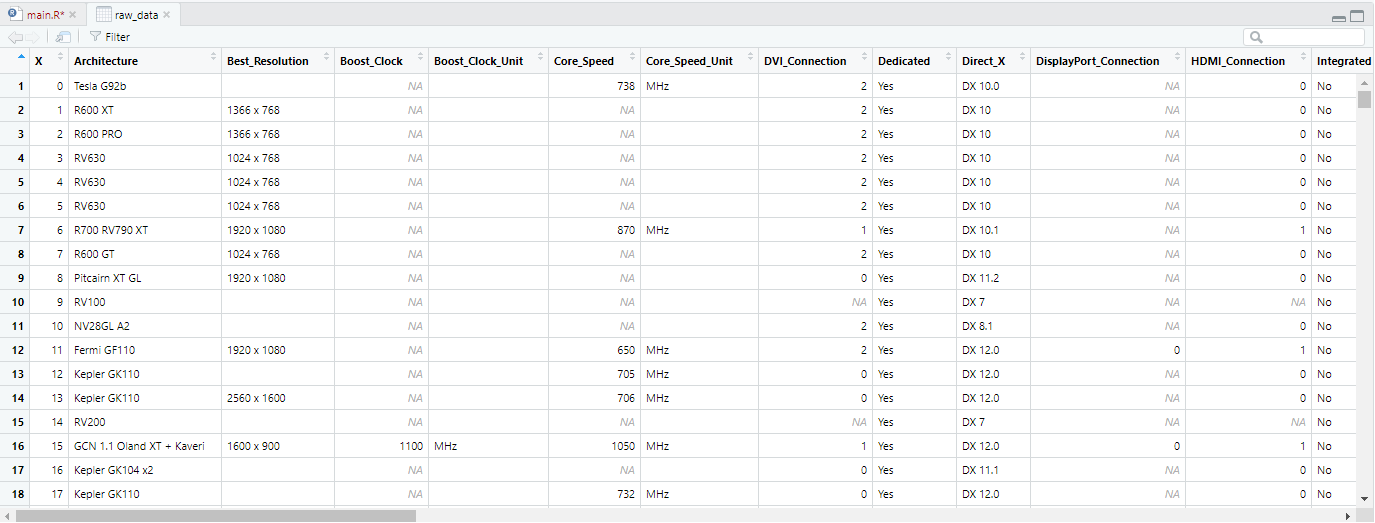
\includegraphics[keepaspectratio, width=1\textwidth, height=1\textheight]{Import/1.png}
\end{figure}


%%%%%%%%%%%%%%%%%%%%%%%%%%%%%%%%%%%%%%%%%%%%%%%%%%%%%%%%%%%%%%%%%%

\section{Data cleaning}
“Cleaning” refers to the process of removing invalid data points from a dataset.\\
Data cleaning is the process of fixing or removing incorrect, corrupted, incorrectly formatted, duplicate, or incomplete data within a dataset. When combining multiple data sources, there are many opportunities for data to be duplicated or mislabeled. If data is incorrect, outcomes and algorithms are unreliable, even though they may look correct. There is no one absolute way to prescribe the exact steps in the data cleaning process because the processes will vary from dataset to dataset.
\subsection{Data extracting}
\begin{figure}[H]
    \centering
    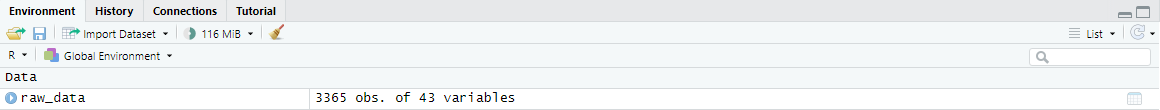
\includegraphics[keepaspectratio, width=1\textwidth, height=1\textheight]{Clean/1.png}
\end{figure}
The dataset has 3365 observation of 43 variables. However, since most of the properties are in object form, we extract 13 variables:
\begin{itemize}
    \item \verb|Manufacturer| 
    \item \verb|Name| 
    \item \verb|Architecture|
    \item \verb|Boost_Clock|
    \item \verb|Core_Speed|
    \item \verb|Max_Power|
    \item \verb|Memory|
    \item \verb|Memory_Bus|
    \item \verb|Memory_Speed|
    \item \verb|Release_Year|
    \item \verb|Release_Price|
    \item \verb|Shader|
    \item \verb|TMUs|
\end{itemize}
from the data frame \verb|raw_data|. Then we create a new data frame \verb|data| by using \verb|select()| function. The \verb|select()| function in \verb|dplyr| package helps us to select the columns based on conditions which are column names of the data frame.
\begin{mdframed}[leftline=false,rightline=false,backgroundcolor=lightblue!10,nobreak=false]
    \begin{minted}[linenos,breaklines,breaksymbolleft=,obeytabs=true,tabsize=2]{R}
data = raw_data %>% select('Manufacturer','Name','Architecture','Boost_Clock','Core_Speed',
'Max_Power','Memory','Memory_Bus', 'Memory_Speed', 'Release_Year', 'Release_Price','Shader','TMUs')
View(data)
    \end{minted}
\end{mdframed}
\begin{figure}[H]
    \centering
    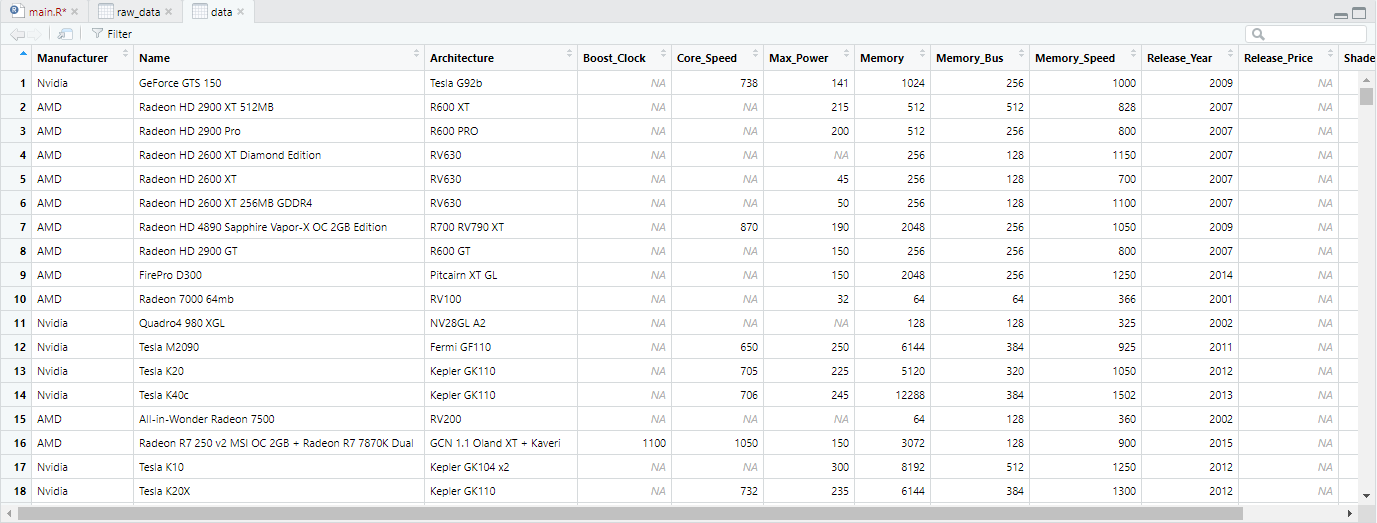
\includegraphics[keepaspectratio, width=1\textwidth, height=1\textheight]{Clean/2.png}
\end{figure}
As shown above we can see that there are places where the value is \texttt{NA} (meaning not available). We will address this problem in the next section.

\subsection{Not available data checking}

As mentioned above, now we have to check \verb|NA| data in the data frame \verb|data|. If there are any \verb|NA| data, find a solution for these \verb|NA| data.\\
There are many ways to handle \verb|NA| values.
\subsubsection{Dropping}
The first method we use here is to eliminate observations which each has at least one \verb|NA| variable to get a new data frame \verb|df_drop| by using \verb|filter()| function combining with \verb|is.na()| function. While \verb|is.na()| fuction indicates which element is \verb|NA| data, the \verb|filter()| function returns rows where conditions are true. Therefore, using \verb|OR| operator helps us eliminate \verb|NA| data. We also use the \verb|summary()| function to summarize.


\begin{mdframed}[leftline=false,rightline=false,backgroundcolor=lightblue!10,nobreak=false]
    \begin{minted}[linenos,breaklines,breaksymbolleft=,obeytabs=true,tabsize=2]{R}
df_drop = data %>% filter(!( is.na(Manufacturer) | is.na(Name) | is.na(Architecture) | is.na(Boost_Clock) | is.na(Core_Speed) | is.na(Max_Power) | is.na(Memory) | is.na(Memory_Bus) | is.na(Memory_Speed) | is.na(Release_Year) | is.na(Release_Price) | is.na(Shader) | is.na(TMUs)))
View(df_drop)
summary(df_drop)
    \end{minted}
\end{mdframed}
\begin{figure}[H]
    \centering
    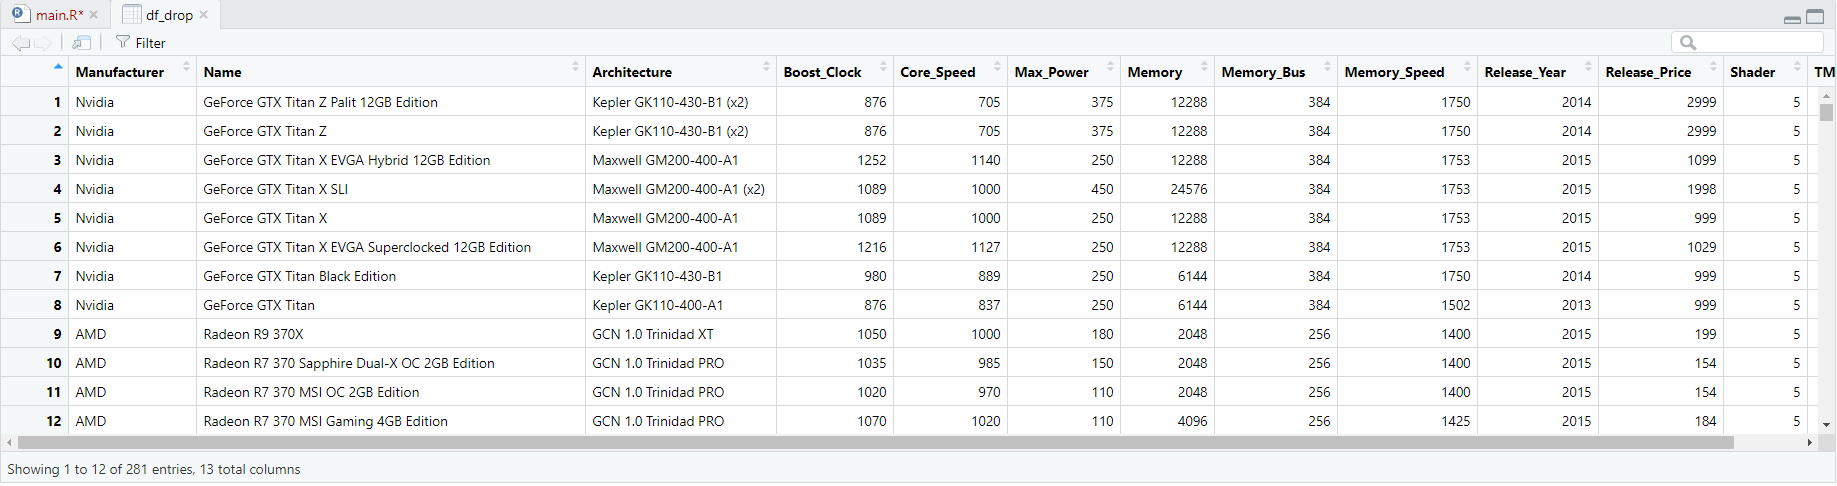
\includegraphics[keepaspectratio, width=1\textwidth, height=1\textheight]{Clean/df_drop.png}
\end{figure}
\begin{figure}[H]
    \centering
    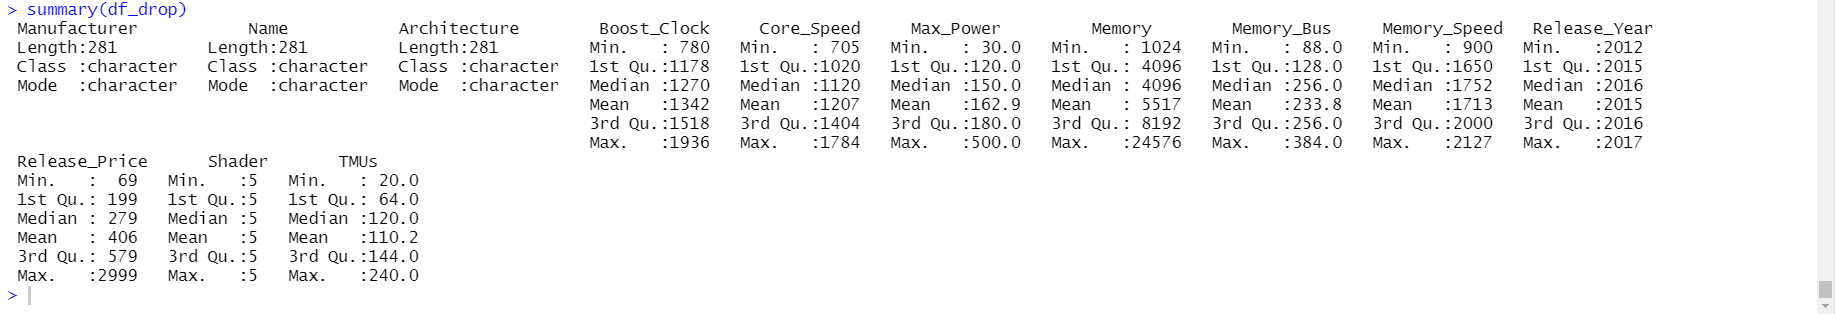
\includegraphics[keepaspectratio, width=1\textwidth, height=1\textheight]{Clean/df_drop_summary.png}
\end{figure}
After filtering, we see that only 281 observations left, compared to the original 3365 observations. That means 3365 - 281 = 3084 observations have at least one \verb|NA| value. And this is not good at all because the very sharp decrease in the number of observations (281 $\ll$ 3365) can lead to skewed results. Thus, we will find another way to handle it.

\subsubsection{Replacing with column mean}
Another method to handle that is to replace the \verb|NA| values present in the data set with the mean. We use the \verb|mutate_all()| function to change these \verb|NA| values by the corresponding mean according to the column that contains them. If a value is NA, it will be replaced with the mean. Otherwise, it will stay the same.
\begin{mdframed}[leftline=false,rightline=false,backgroundcolor=lightblue!10,nobreak=false]
    \begin{minted}[linenos,breaklines,breaksymbolleft=,obeytabs=true,tabsize=2]{R}
df_mean = data %>% mutate_all(~ifelse(is.na(.x), mean(.x, na.rm = TRUE), .x))       
View(df_mean)
summary(df_mean)
    \end{minted}
\end{mdframed}
\begin{figure}[H]
    \centering
    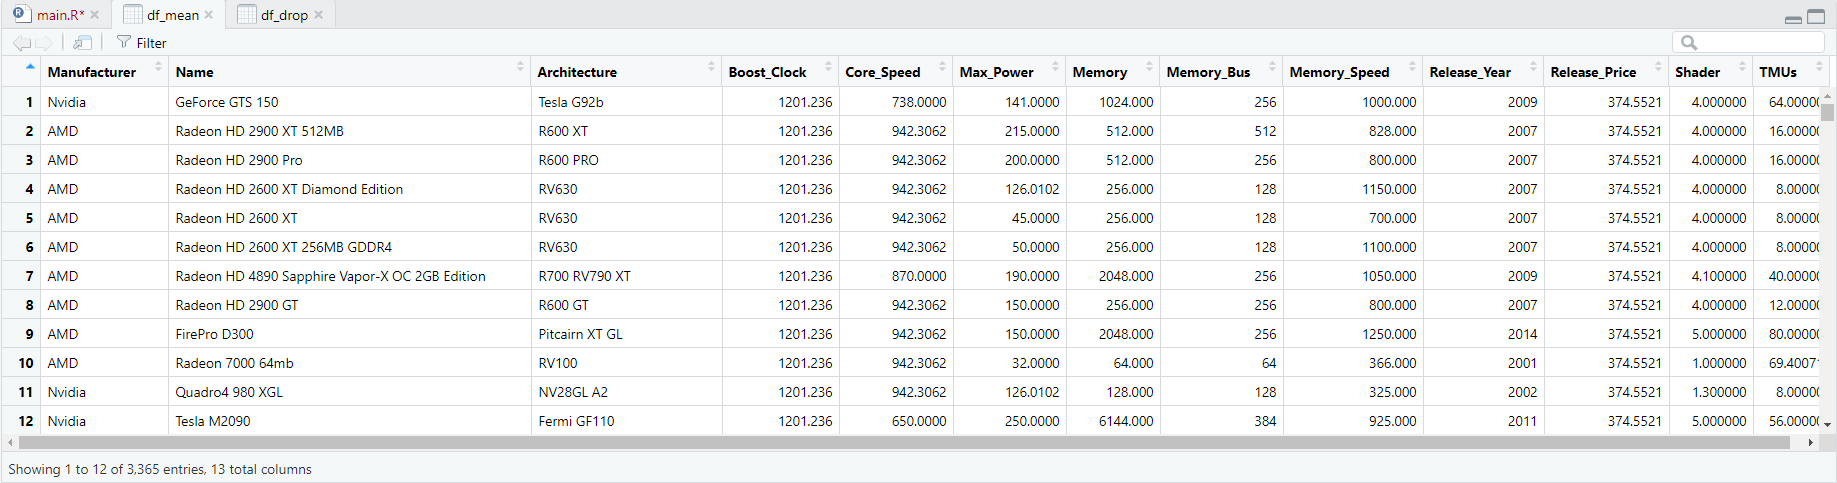
\includegraphics[keepaspectratio, width=1\textwidth, height=1\textheight]{Clean/df_mean.png}
\end{figure}
\begin{figure}[H]
    \centering
    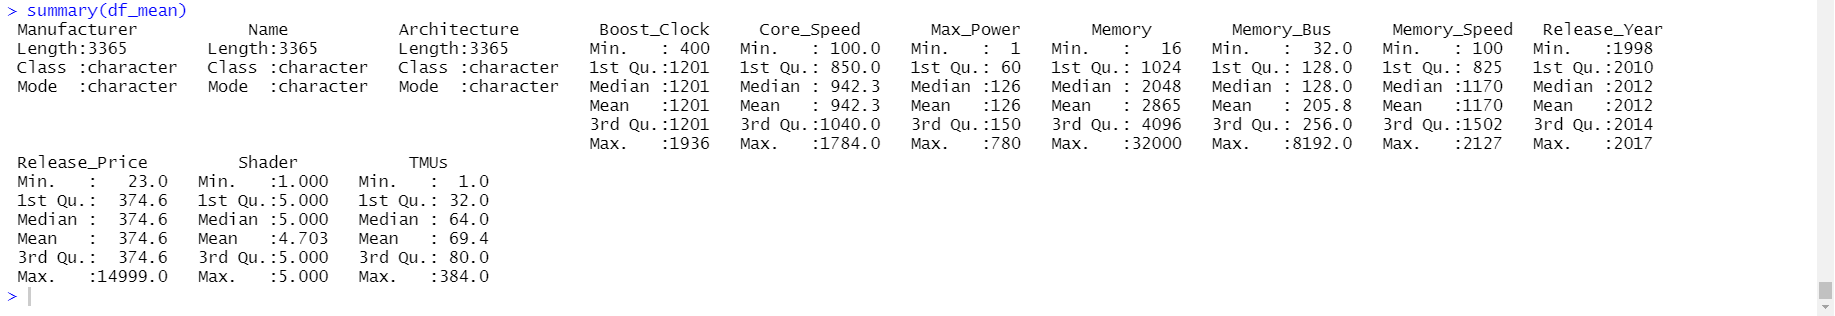
\includegraphics[keepaspectratio, width=1\textwidth, height=1\textheight]{Clean/df_mean_summary.png}
\end{figure}
The result this time is very good because we can both keep the number of observations in the data set and deal with the \verb|NA| values.
\subsubsection{Replacing with column median}
In this section we will do the same as above but change the mean to the median.
\begin{mdframed}[leftline=false,rightline=false,backgroundcolor=lightblue!10,nobreak=false]
    \begin{minted}[linenos,breaklines,breaksymbolleft=,obeytabs=true,tabsize=2]{R}
df_median = data %>% mutate_all(~ifelse(is.na(.x), median(.x, na.rm = TRUE), .x))       
View(df_median)
summary(df_median)
    \end{minted}
\end{mdframed}
\begin{figure}[H]
    \centering
    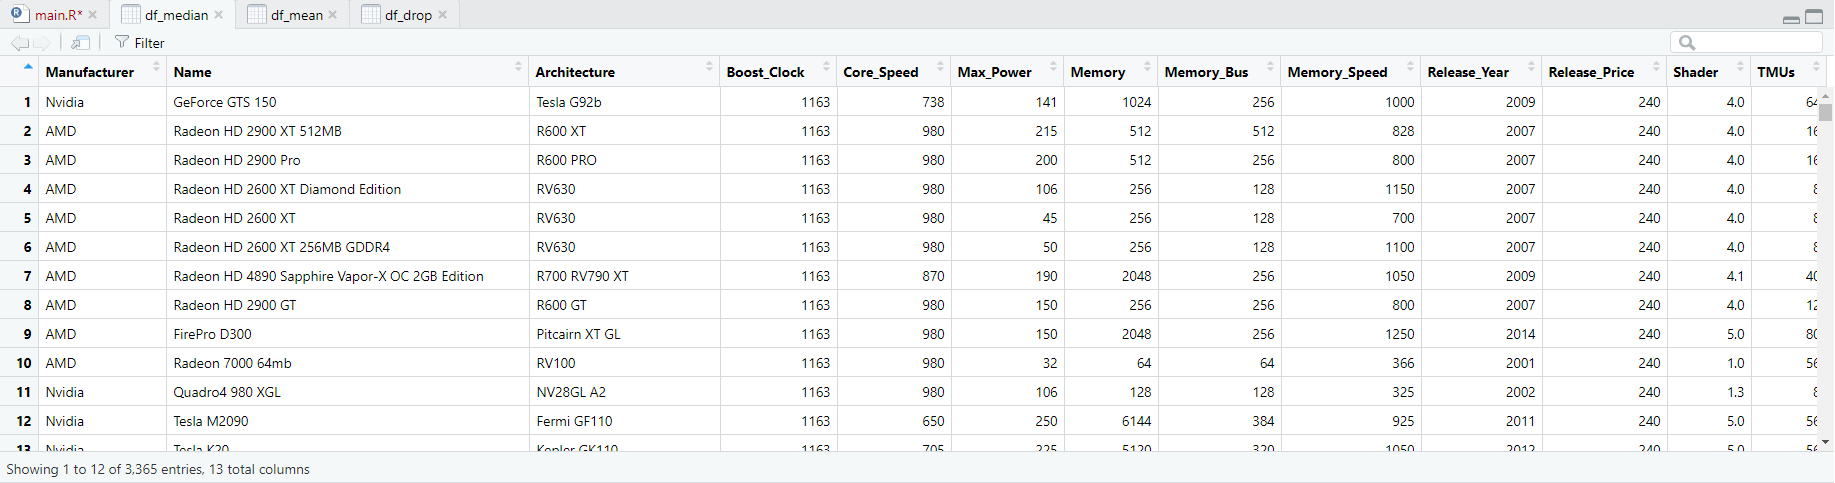
\includegraphics[keepaspectratio, width=1\textwidth, height=1\textheight]{Clean/df_median.png}
\end{figure}
\begin{figure}[H]
    \centering
    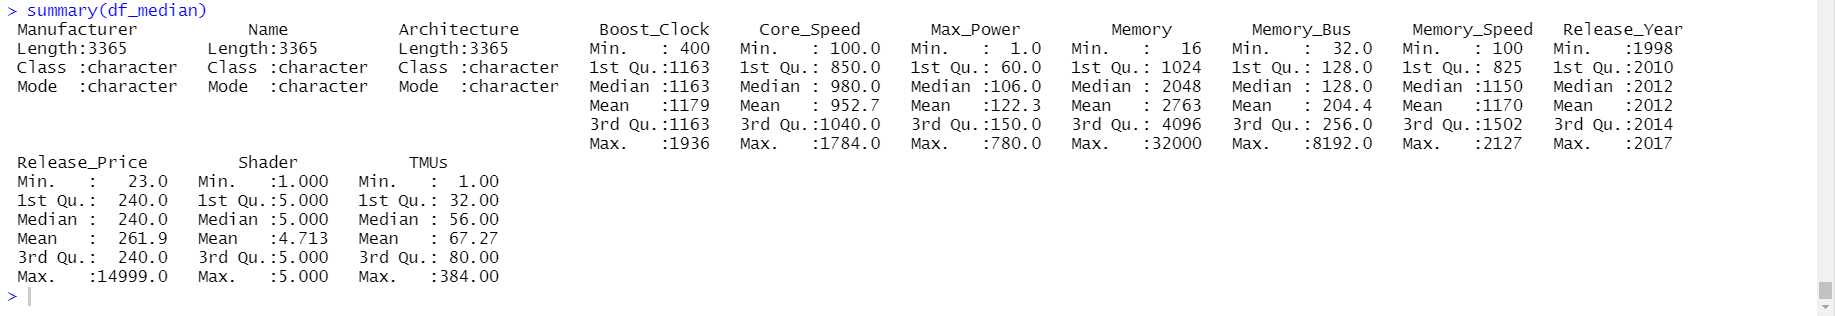
\includegraphics[keepaspectratio, width=1\textwidth, height=1\textheight]{Clean/df_median_summary.png}
\end{figure}
\subsubsection{Replacing with \textit{k}-NN}
\subsubsubsection{Fast introduction to \textit{k}-NN}
A popular approach to missing data imputation is to use a model to predict the missing values.\\\\
This requires a model to be created for each input variable that has missing values. Although any one among a range of different models can be used to predict the missing values, the \textit{k}-nearest neighbor (\textit{k}-NN) algorithm has proven to be generally effective, often referred to as “nearest neighbor imputation”. It can be used for data that are continuous, discrete, ordinal and categorical which makes it particularly useful for dealing with all kind of missing data.\\\\
The idea in \textit{k}-NN methods is to identify \textit{k} samples in the dataset that are similar or close in the space. Then we use these \textit{k} samples to estimate the value of the missing data points. Each sample’s missing values are imputed using the mean value of the \textit{k}-neighbors found in the dataset. The assumption behind using \textit{k}-NN for missing values is that a point value can be approximated by the values of the points that are closest to it, based on other variables.\\\\
The nearest, most similar, neighbours are found by minimising a distance function, usually the $Euclidean$ $distance$ \footnote{There are also some other methods such as Hamming distance, Manhattan distance and Minkowski distance.}\:, defined as \cite{bib5}:
\begin{equation*}
    E(a,b) = \sqrt{\sum_{i \in D}(x_{ai} - x_{bi})^2} 
\end{equation*}
where:
\begin{itemize}
    \item $E(a, b)$ is the distance between the two cases $a$ and $b$.
    \item $x_{ai}$ and $x_{bi}$ are the values of attribute $i$ in cases $a$ and $b$ respectively.
    \item $D$ is the set of attributes with non-missing values in both cases.
\end{itemize}
\textit{k}-NN algorithm has the following basic steps:
\begin{enumerate}
    \item Calculate distance.
    \item Find closest neighbors.
    \item Vote for labels.
\end{enumerate}
\subsubsubsection{Applying to dataset}
For our dataset, we choose \textit{k} (number of nearest neighbours used) = square root of the number of observations present in the dataset (3365). 
\begin{mdframed}[leftline=false,rightline=false,backgroundcolor=lightblue!10,nobreak=false]
    \begin{minted}[linenos,breaklines,breaksymbolleft=,obeytabs=true,tabsize=2]{R}
df_knn <- kNN(data, k = sqrt(nrow(data)), imp_var = FALSE)
View(df_knn)
summary(df_knn)
    \end{minted}
\end{mdframed}
\begin{figure}[H]
    \centering
    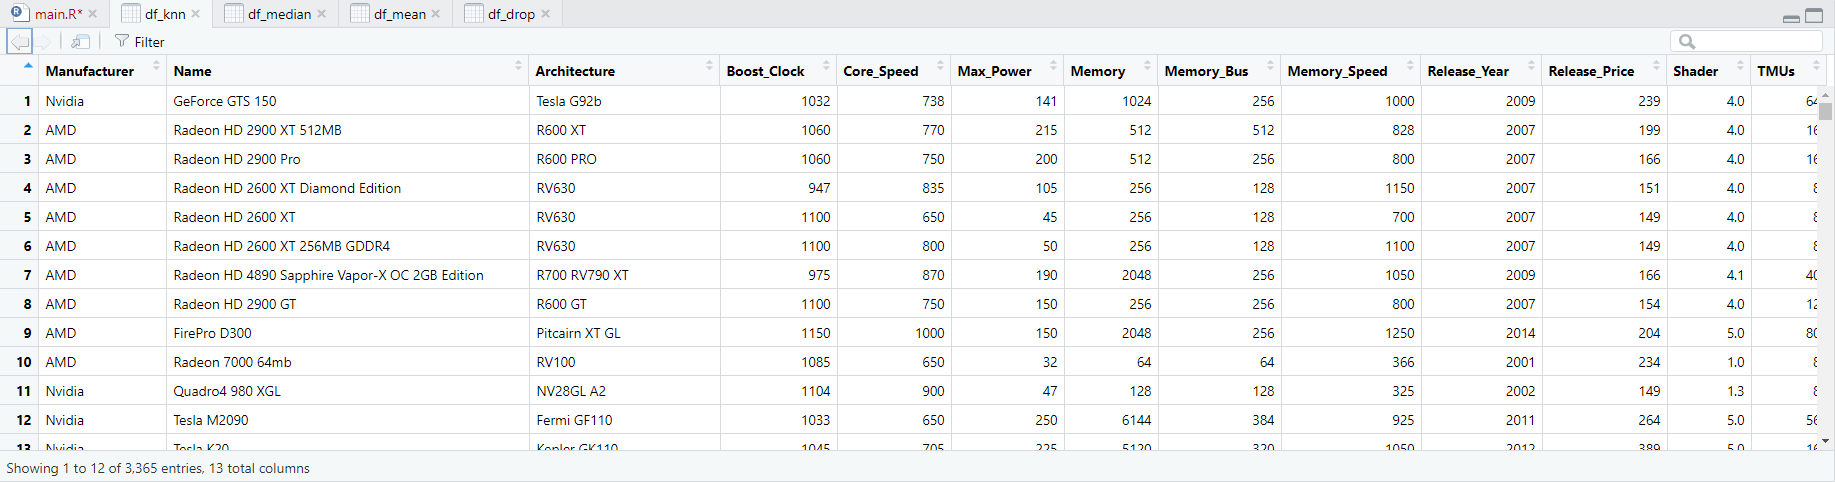
\includegraphics[keepaspectratio, width=1\textwidth, height=1\textheight]{Clean/df_knn.png}
\end{figure}
\begin{figure}[H]
    \centering
    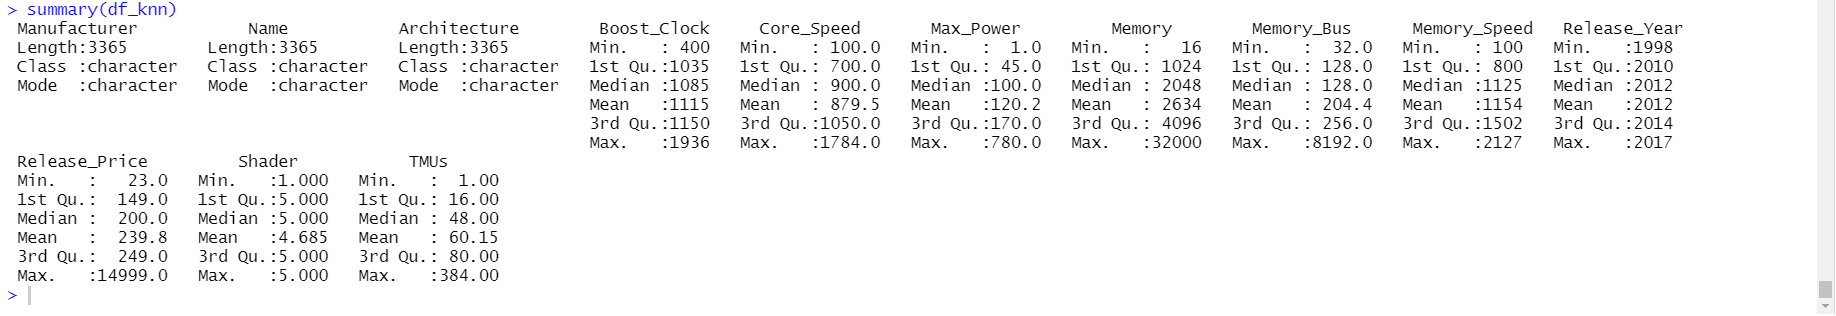
\includegraphics[keepaspectratio, width=1\textwidth, height=1\textheight]{Clean/df_knn_summary.png}
\end{figure}
In our project, we will use this data frame \verb|df_knn|. And from this section onwards, the processing data frame is named \verb|df|.
\begin{mdframed}[leftline=false,rightline=false,backgroundcolor=lightblue!10,nobreak=false]
    \begin{minted}[linenos,breaklines,breaksymbolleft=,obeytabs=true,tabsize=2]{R}
df = df_knn
    \end{minted}
\end{mdframed}
The reason we chose \textit{k}-NN is because this algorithm can compete with the most accurate models as it gives highly accurate predictions.\\\\
The \textit{k}-NN algorithm is a type of lazy learning, where the computation for the generation of the predictions is deferred until classification. Although this method increases the costs of computation compared to other algorithms, \textit{k}-NN is still the better choice for applications where predictions are not requested frequently but where accuracy is important.
%%%%%%%%%%%%%%%%%%%%%%%%%%%%%%%%%%%%%%%%%%%%%%%%%%%%%%%%%%%%%%%%%%

\section{Data visualization}
Data visualization is the graphical representation of information and data. By using visual elements like charts, graphs, and maps, data visualization tools provide an accessible way to see and understand trends, outliers, and patterns in data.
\subsection{Transformation}
Logarithm transformation \cite{bib6} is a data transformation method in which it replaces each variable $x$ with a $log(x)$. The choice of the logarithm base is usually left up to the analyst and it would depend on the purposes of statistical modeling.\\\\
When our original continuous data do not follow the bell curve, we can log transform this data to make it as “normal” as possible so that the statistical analysis results from this data become more valid.\\\\
Therefore, we decided to convert the data to a logarithmic equation of the form:
\begin{equation*}
    f(x) = log(x)
\end{equation*}
where:
\begin{itemize}
    \item $x$: Values in our dataset.
\end{itemize}
We create new variable columns corresponding to the variable columns present in the dataset. And then add them in the data frame \verb|df|. We use \verb|log()| function:
\begin{mdframed}[leftline=false,rightline=false,backgroundcolor=lightblue!10,nobreak=false]
    \begin{minted}[linenos,breaklines,breaksymbolleft=,obeytabs=true,tabsize=2]{R}
df['log.Boost_Clock'] <- log(df['Boost_Clock'])
df['log.Core_Speed'] <- log(df['Core_Speed'])
df['log.Max_Power'] <- log(df['Max_Power'])
df['log.Memory'] <- log(df['Memory'])
df['log.Memory_Bus'] <- log(df['Memory_Bus'])
df['log.Memory_Speed'] <- log(df['Memory_Speed'])
df['log.Release_Year'] <- log(df['Release_Year'])
df['log.Release_Price'] <- log(df['Release_Price'])
df['log.Shader'] <- log(df['Shader'])
df['log.TMUs'] <- log(df['TMUs'])
View(df)
    \end{minted}
\end{mdframed}
\begin{figure}[H]
    \centering
    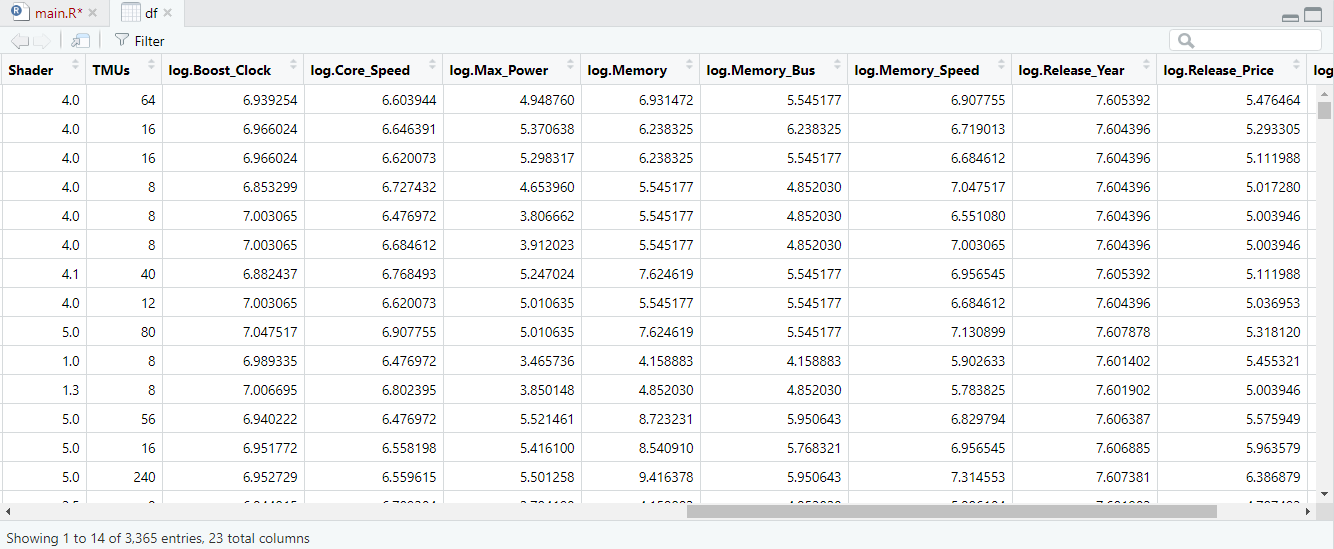
\includegraphics[keepaspectratio, width=1\textwidth, height=1\textheight]{Visualization/Transformation/1.png}
\end{figure}
And from this step onwards, we will use logarithmic values for calculations as well as comparisons.
\subsection{Descriptive statistics for each of the variables}
For this section, we make a new data frame named \verb|stats_table| to calculate mean, max, min, median and standard deviation for each variable. 
\begin{mdframed}[leftline=false,rightline=false,backgroundcolor=lightblue!10,nobreak=false]
    \begin{minted}[linenos,breaklines,breaksymbolleft=,obeytabs=true,tabsize=2]{R}
stats_table = data.frame(
  Name = c('mean', 'median', 'sd', 'min', 'max'),
  log.Boost_Clock = c(mean(df[, 'log.Boost_Clock']), median(df[, 'log.Boost_Clock']), sd(df[, 'log.Boost_Clock']), min(df[, 'log.Boost_Clock']), max(df[, 'log.Boost_Clock'])),
  log.Core_Speed = c(mean(df[, 'log.Core_Speed']), median(df[, 'log.Core_Speed']), sd(df[, 'log.Core_Speed']), min(df[, 'log.Core_Speed']), max(df[, 'log.Core_Speed'])),
  log.Max_Power = c(mean(df[, 'log.Max_Power']), median(df[, 'log.Max_Power']), sd(df[, 'log.Max_Power']), min(df[, 'log.Max_Power']), max(df[, 'log.Max_Power'])),
  log.Memory = c(mean(df[, 'log.Memory']), median(df[, 'log.Memory']), sd(df[, 'log.Memory']), min(df[, 'log.Memory']), max(df[, 'log.Memory'])),
  log.Memory_Bus = c(mean(df[, 'log.Memory_Bus']), median(df[, 'log.Memory_Bus']), sd(df[, 'log.Memory_Bus']), min(df[, 'log.Memory_Bus']), max(df[, 'log.Memory_Bus'])),
  log.Memory_Speed = c(mean(df[, 'log.Memory_Speed']), median(df[, 'log.Memory_Speed']), sd(df[, 'log.Memory_Speed']), min(df[, 'log.Memory_Speed']), max(df[, 'log.Memory_Speed'])),
  log.Release_Year = c(mean(df[, 'log.Release_Year']), median(df[, 'log.Release_Year']), sd(df[, 'log.Release_Year']), min(df[, 'log.Release_Year']), max(df[, 'log.Release_Year'])),
  log.Release_Price = c(mean(df[, 'log.Release_Price']), median(df[, 'log.Release_Price']), sd(df[, 'log.Release_Price']), min(df[, 'log.Release_Price']), max(df[, 'log.Release_Price'])),
  log.Shader = c(mean(df[, 'log.Shader']), median(df[, 'log.Shader']), sd(df[, 'log.Shader']), min(df[, 'log.Shader']), max(df[, 'log.Shader'])),
  log.TMUs = c(mean(df[, 'log.TMUs']), median(df[, 'log.TMUs']), sd(df[, 'log.TMUs']), min(df[, 'log.TMUs']), max(df[, 'log.TMUs']))
)
View(stats_table)
    \end{minted}
\end{mdframed}
\begin{figure}[H]
    \centering
    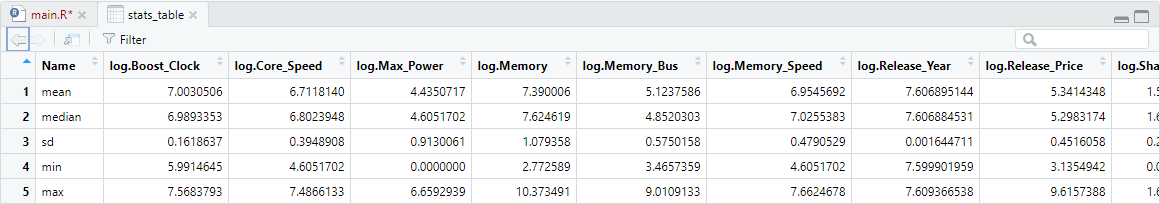
\includegraphics[keepaspectratio, width=1\textwidth, height=1\textheight]{Visualization/Descriptive/2.png}
\end{figure}
We can also try to create a frequency table for \verb|Shader| based on what we observed.
\begin{mdframed}[leftline=false,rightline=false,backgroundcolor=lightblue!10,nobreak=false]
    \begin{minted}[linenos,breaklines,breaksymbolleft=,obeytabs=true,tabsize=2]{R}
ftable(df[ ,'Shader'])
    \end{minted}
\end{mdframed}
\begin{lstlisting}
 1  1.1  1.3  1.4    2  2.5    3    4  4.1 4.55    5
                                                       
 1    4   14    9   59    2  174  273  170    1 2658
\end{lstlisting}

\subsection{Graphs}
Note that all graphs in this report are in pdf format. So, if the letters or numbers or symbols are too small, or the chart is blurry, please zoom in for a better view.
\subsubsection{Hist}
A histogram is a graphical representation that organizes a group of data points into user-specified ranges. Similar in appearance to a bar graph, the histogram condenses a data series into an easily interpreted visual by taking many data points and grouping them into logical ranges or bins.
\begin{mdframed}[leftline=false,rightline=false,backgroundcolor=lightblue!10,nobreak=false]
    \begin{minted}[linenos,breaklines,breaksymbolleft=,obeytabs=true,tabsize=2]{R}
hist(df$Release_Price, main="Histogram of Release_Price", xlab = "US Dollar", ylab = "Number of GPUs", col = rainbow(10), breaks=100)
hist(df$log.Release_Price, main = "Histogram of log.Release_Price", xlab = "log(US Dollar)", ylab = "Number of GPUs", col = rainbow(length(unique(df$log.Release_Price))), breaks=100)
    \end{minted}
\end{mdframed}

\begin{center}
\begin{adjustbox}{width=\textwidth}
    \begin{tabular}{cc}
        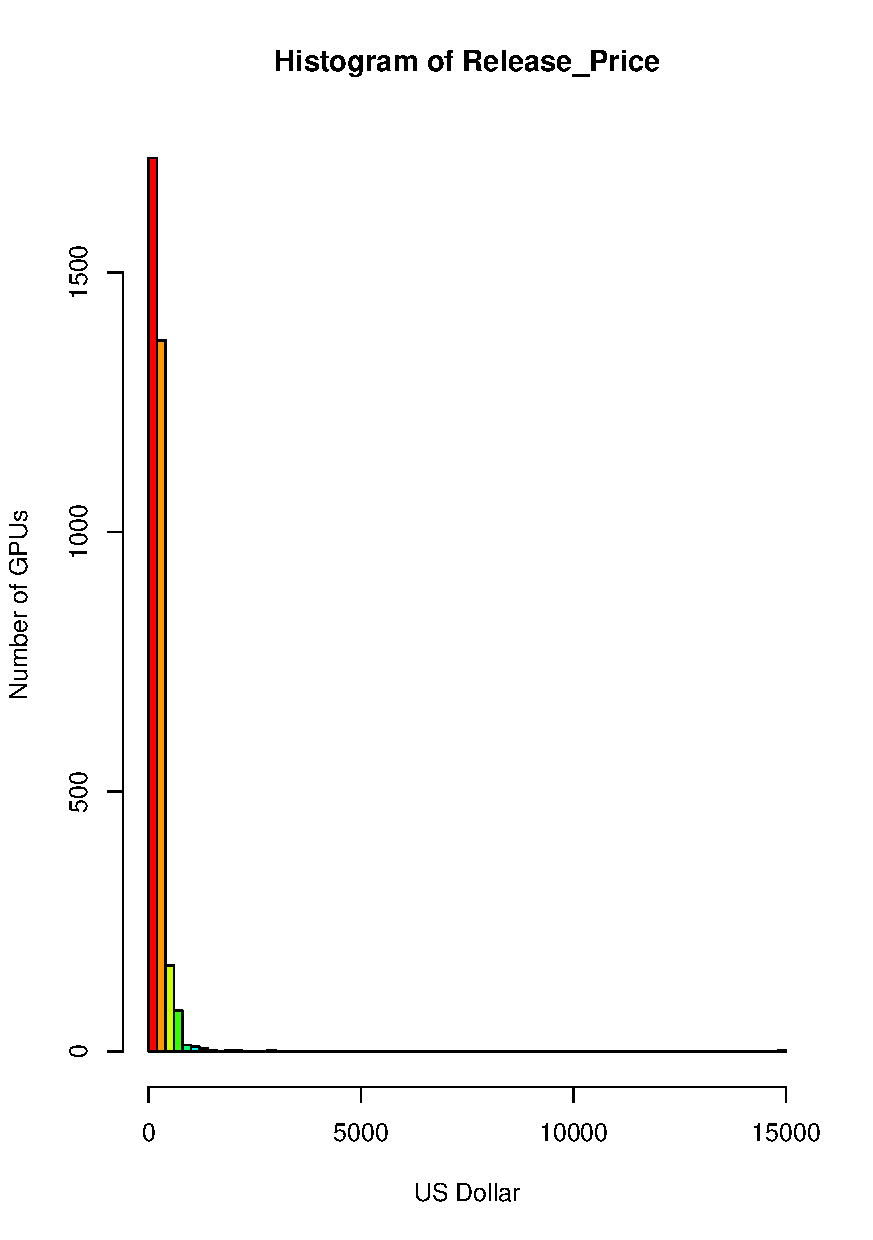
\includegraphics[keepaspectratio, width=1\textwidth, height=1\textheight]{Visualization/Hist/release_price.pdf}
        &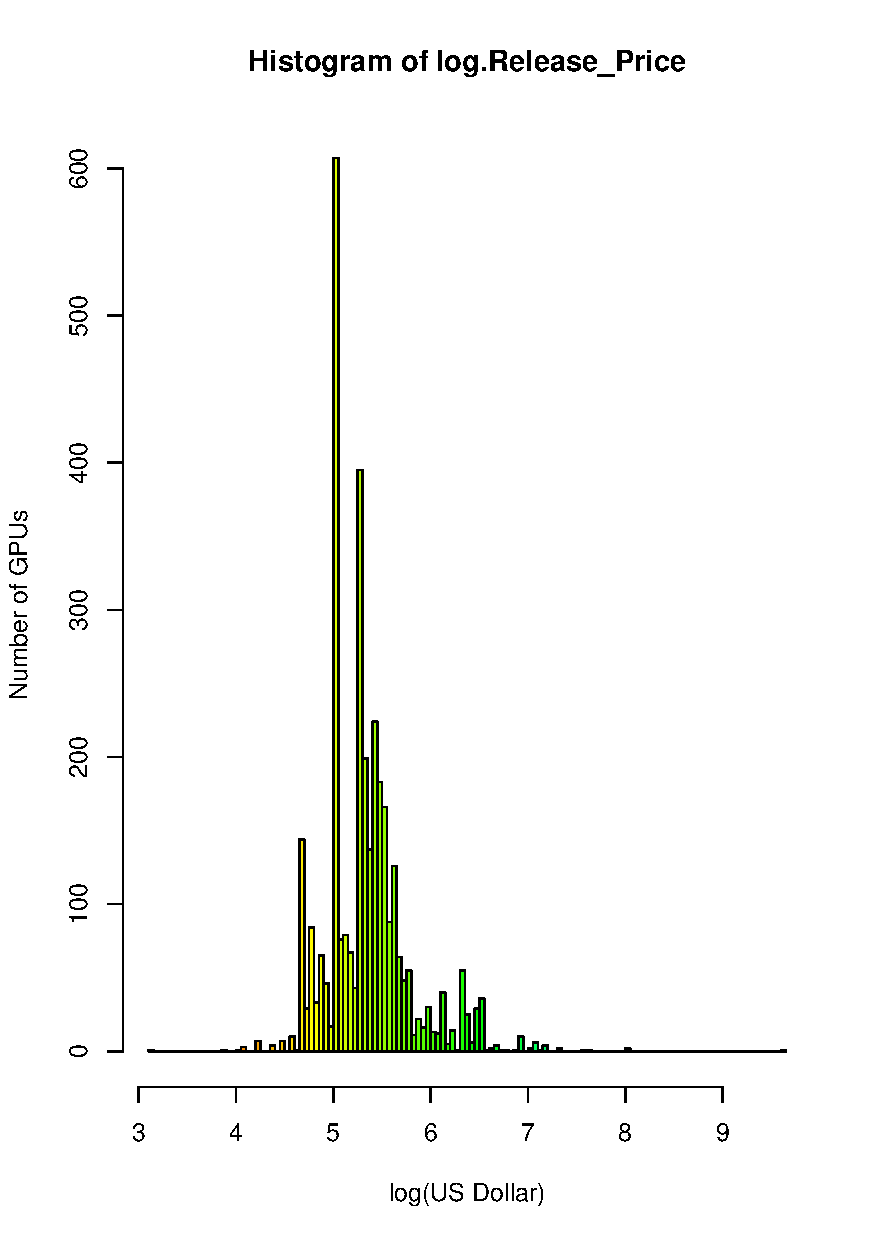
\includegraphics[keepaspectratio, width=1\textwidth, height=1\textheight]{Visualization/Hist/log.release_price.pdf}
    \end{tabular}
\end{adjustbox}
\end{center}
We can easily see the benefits of data transformation. It helps our data to focus on certain area rather than discretely distributed. Try again with \verb|Release_Year|.
\begin{mdframed}[leftline=false,rightline=false,backgroundcolor=lightblue!10,nobreak=false]
    \begin{minted}[linenos,breaklines,breaksymbolleft=,obeytabs=true,tabsize=2]{R}
hist(df$Release_Year, main="Histogram of Release_Year", xlab = "Year", ylab = "Number of GPUs", col = rainbow(20), breaks = 20, xlim=c(1998,2017))
hist(df$log.Release_Year, main = "Histogram of log.(Release_Year)", xlab = "log(Year)", ylab = "Number of GPUs", col = rainbow(20), breaks = 20)
    \end{minted}
\end{mdframed}
\begin{center}
\begin{adjustbox}{width=1\textwidth}
    \begin{tabular}{cc}
        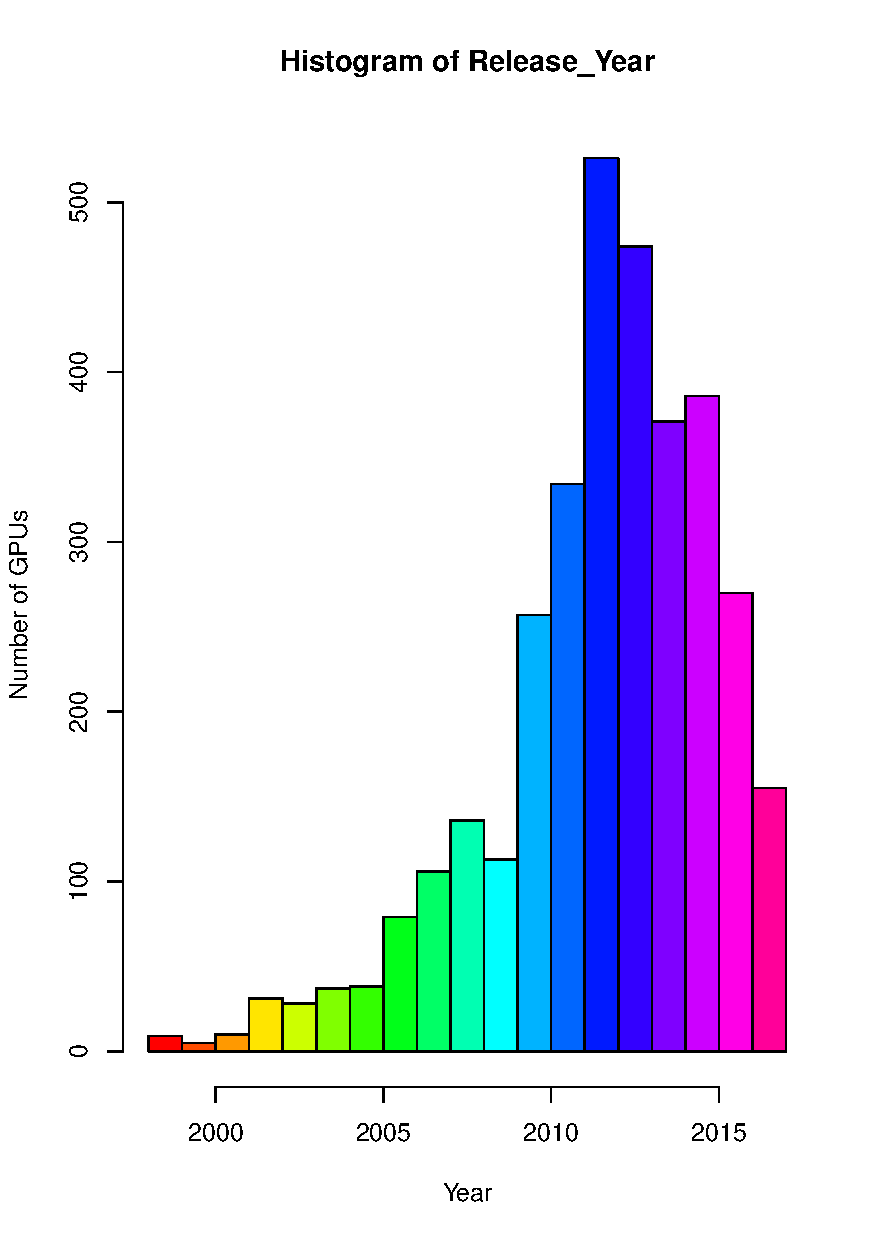
\includegraphics[keepaspectratio, width=1\textwidth, height=1\textheight]{Visualization/Hist/release_year.pdf}
        &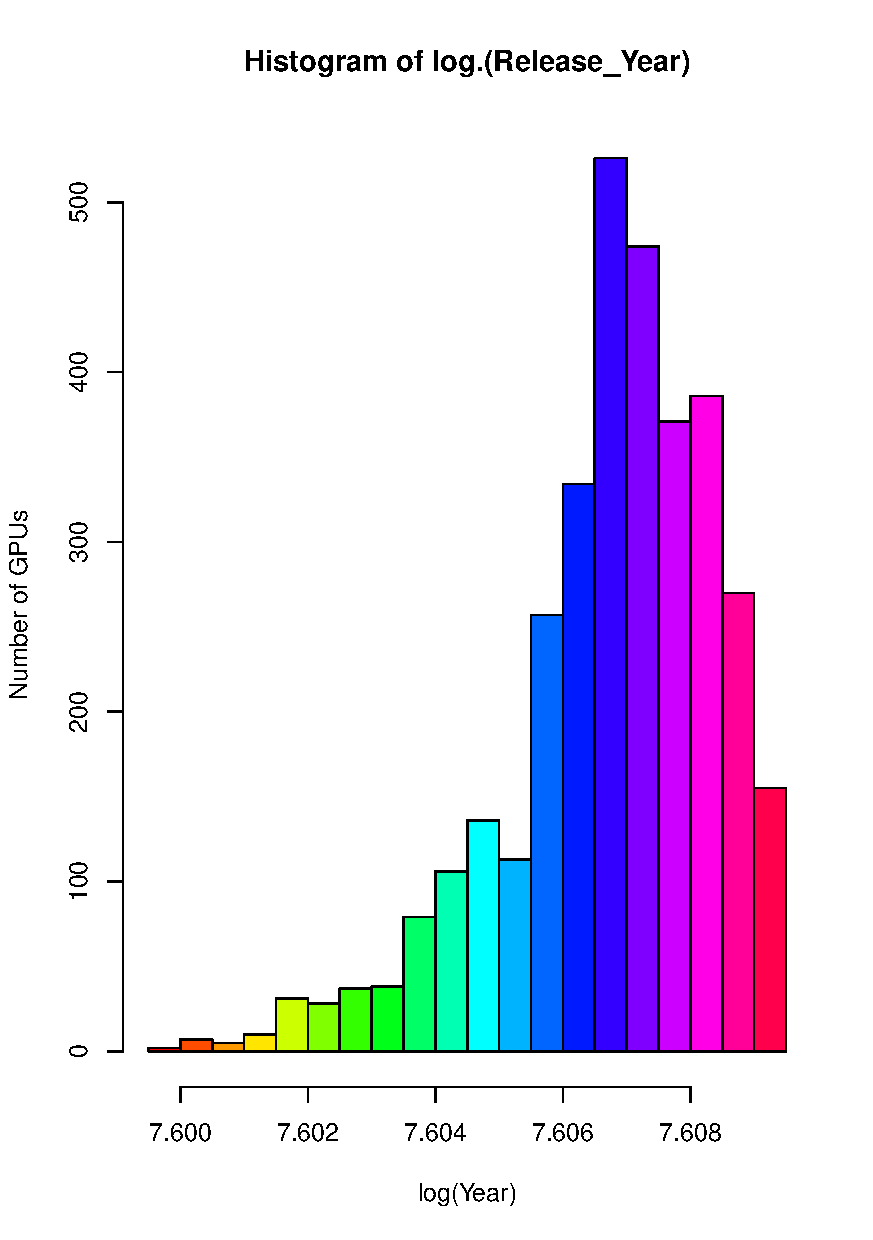
\includegraphics[keepaspectratio, width=1\textwidth, height=1\textheight]{Visualization/Hist/log.release_year.pdf}
    \end{tabular}
\end{adjustbox}
\end{center}
In this case we can see that both graphs are quite similar. So we can draw the conclusion that data transformation is not always the best way.\\\\
We can use the \verb|ggplot()| function to both view the histogram and view the distribution shape of the dataset.
\begin{mdframed}[leftline=false,rightline=false,backgroundcolor=lightblue!10,nobreak=false]
    \begin{minted}[linenos,breaklines,breaksymbolleft=,obeytabs=true,tabsize=2]{R}
ggplot(df, aes(x = Release_Year, y=..density..)) + theme_classic() +  geom_density() +
  geom_histogram(bins = 50, fill = 'steelblue', color = 'black') + 
  labs(title = 'Histogram of Release_Year', x = 'Year', y = 'Frequency') +
  theme(legend.position='bottom', plot.title = element_text(hjust = 0.5)) 
    \end{minted}
\end{mdframed}  
\begin{figure}[H]
    \centering
    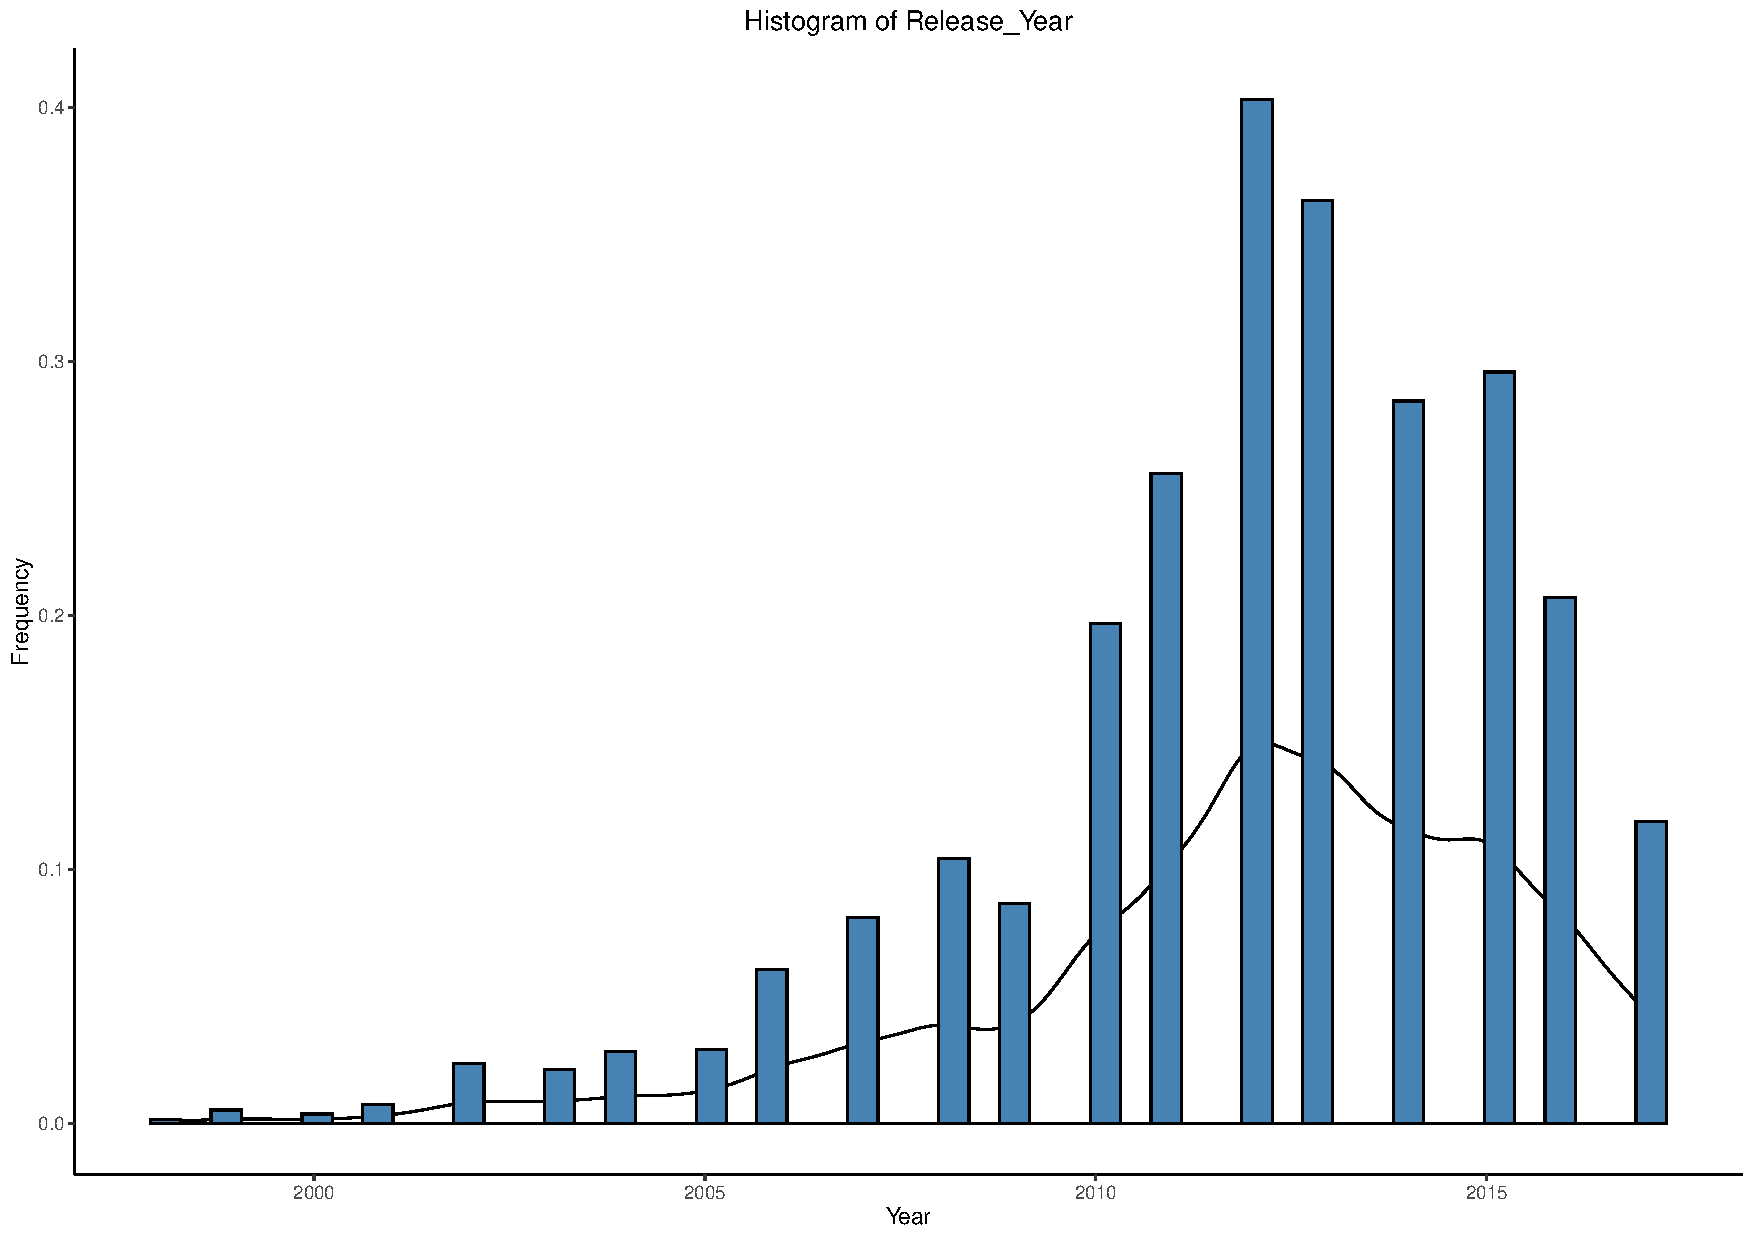
\includegraphics[keepaspectratio, width=1\textwidth, height=1\textheight]{Visualization/Hist/release_year_dis.pdf}
\end{figure}
\subsubsection{Boxplot}
In descriptive statistics, a box plot or boxplot (also known as box and whisker plot) is a type of chart often used in explanatory data analysis. Box plots visually show the distribution of numerical data and skewness through displaying the data quartiles (or percentiles) and averages.\\
Box plots show the seven-number summary of a set of data: 
\begin{itemize}
    \item Minimum score: The lowest score, excluding outliers (shown at the end of the left whisker).
    \item First (lower) quartile: 25\% percent of scores fall below the lower quartile value.
    \item Median: The median marks the mid-point of the data and is shown by the line that divides the box into two parts (sometimes known as the second quartile). Half the scores are greater than or equal to this value and half are less.
    \item Third (upper) quartile: 75\% of the scores fall below the upper quartile value. Thus, 25\% of data are above this value.
    \item Maximum score: The highest score, excluding outliers (shown at the end of the right whisker).
    \item Whiskers: The upper and lower whiskers represent scores outside the middle 50\% (i.e. the lower 25\% of scores and the upper 25\% of scores).
    \item The Interquartile Range (or IQR): This is the box plot showing the middle 50\% of scores (i.e. the range between the 25th and 75th percentile).
\end{itemize}
\begin{mdframed}[leftline=false,rightline=false,backgroundcolor=lightblue!10,nobreak=false]
    \begin{minted}[linenos,breaklines,breaksymbolleft=,obeytabs=true,tabsize=2]{R}
boxplot(df$log.Release_Price ~ df$log.Shader , main="Boxplot of log.Release_Price and log.Shader", ylab = "log.Release_Price", xlab = "log.Shader", col = rainbow (11))
boxplot(df$log.Memory ~ df$log.Memory_Bus, main = "Boxplot of log.Memory and log.Memory_Bus", ylab = "log.Memory", xlab = "log.Memory_Bus", col = rainbow (17))
boxplot(df$log.Memory_Speed ~ df$log.Memory_Bus, main = "Boxplot of log.Memory_Speed and log.Memory_Bus", ylab = "log.Memory_Speed", xlab = "log.Memory_Bus", col = rainbow (17))
    \end{minted}
\end{mdframed}
\begin{figure}[H]
    \centering
    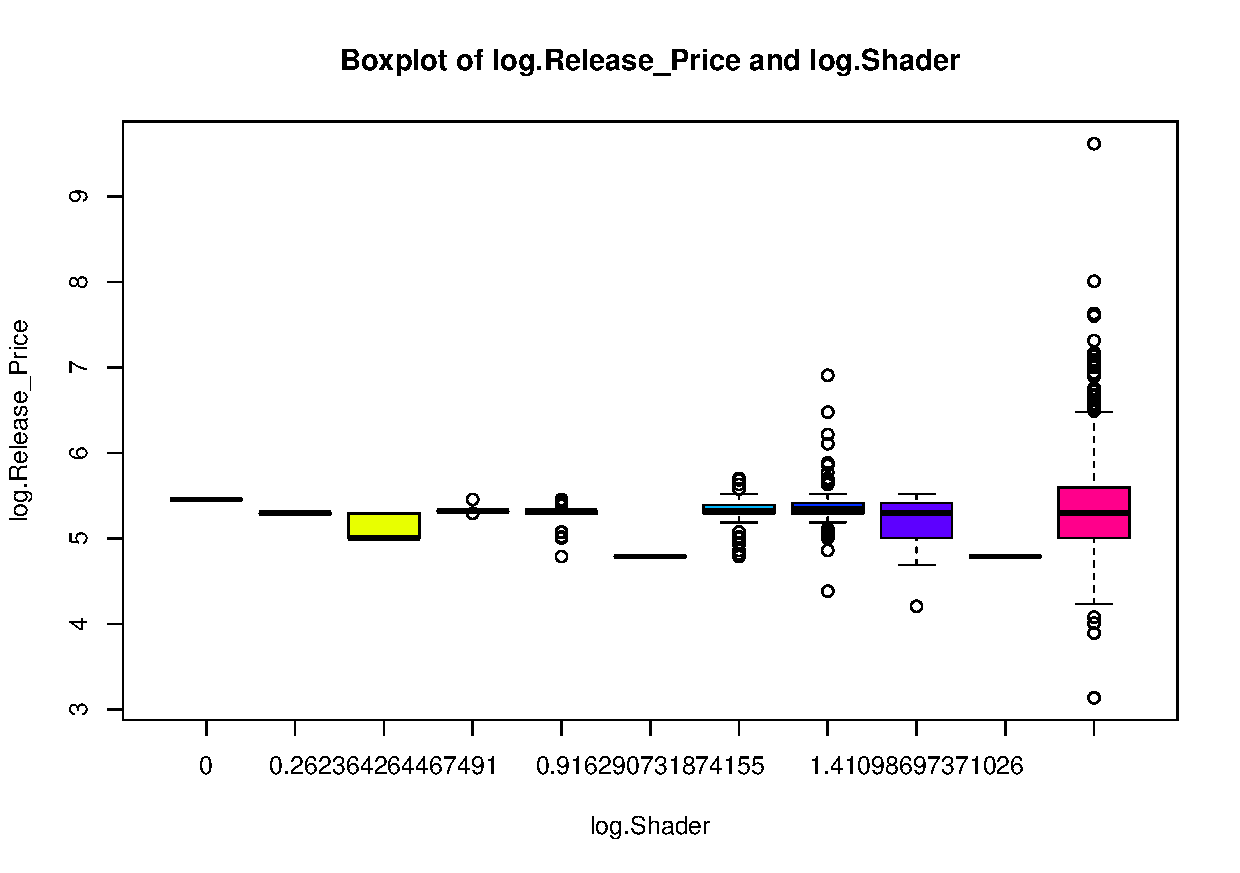
\includegraphics[keepaspectratio, width=1\textwidth, height=1\textheight]{Visualization/Boxplot/price_shader.pdf}
\end{figure}
In boxplot, the black line stands for median value, the top and bottom of the box combined make the interquartile range. The dotted lines stretching both direction from the box (whiskers) is the range, and the small circles outside the range are outliers.
\begin{center}
\begin{adjustbox}{width=\textwidth}
    \begin{tabular}{cc}
        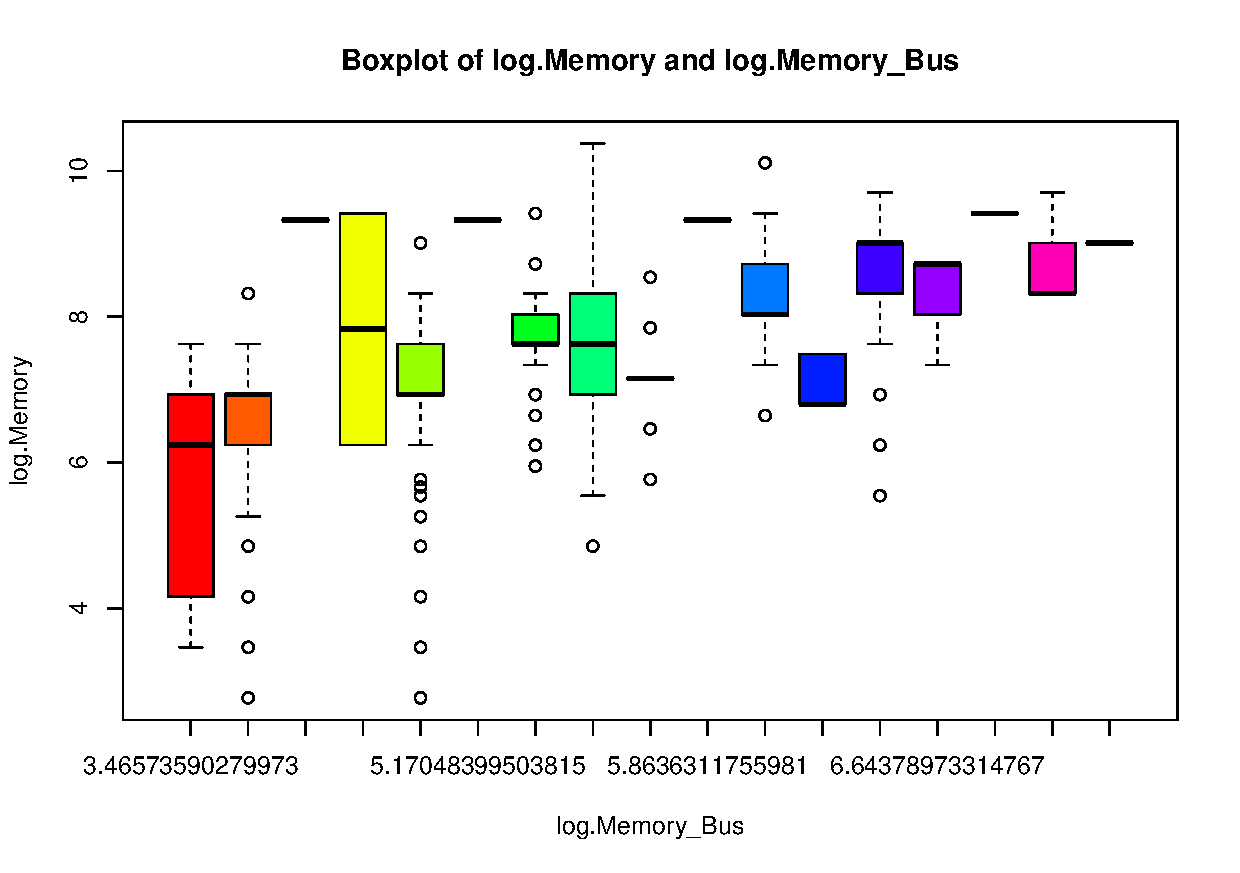
\includegraphics[keepaspectratio, width=1\textwidth, height=1\textheight]{Visualization/Boxplot/mem_bus.pdf} 
        &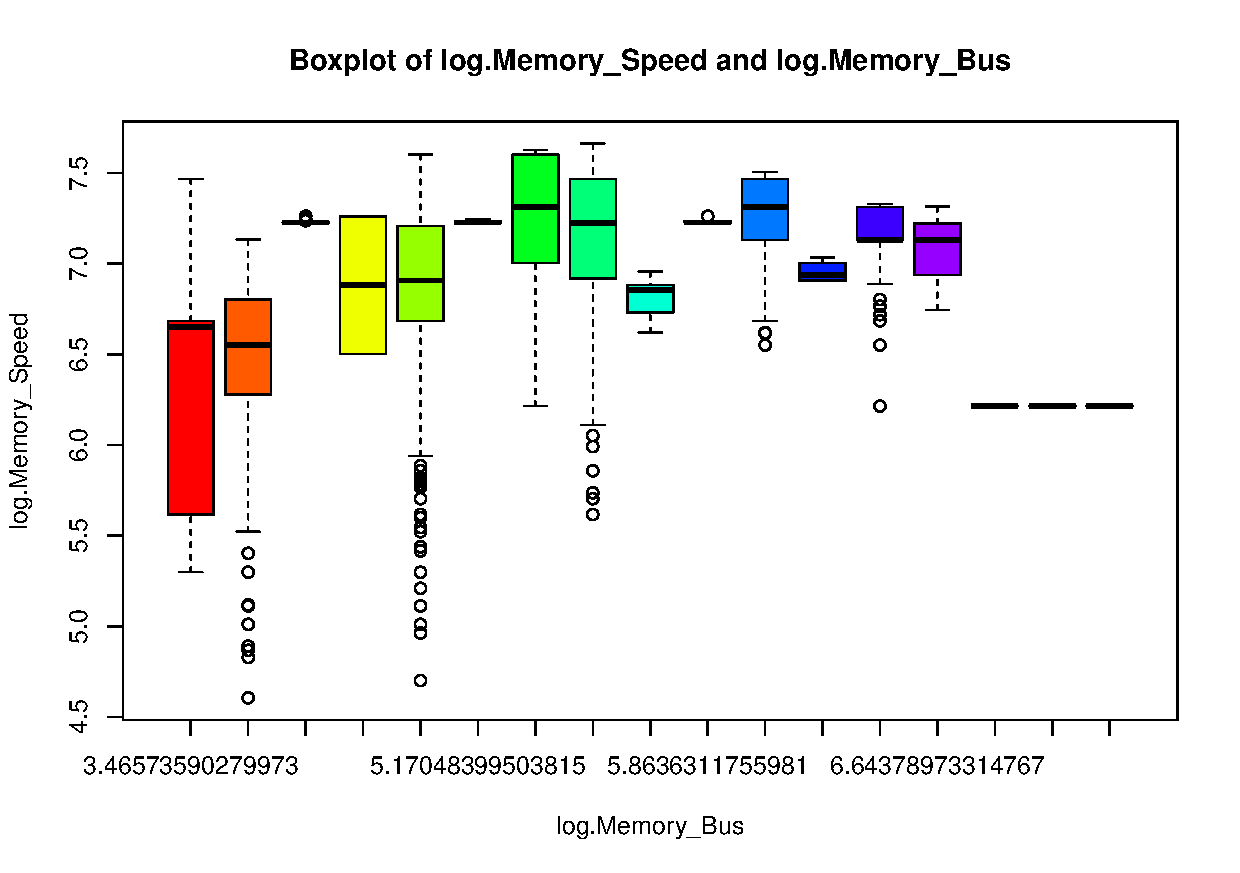
\includegraphics[keepaspectratio, width=1\textwidth, height=1\textheight]{Visualization/Boxplot/mem_speed_bus.pdf}
    \end{tabular}
\end{adjustbox}
\end{center}
\subsubsection{Pairs}
A pairs plot allows to see both distribution of single variables and relationships between two variables. It is a grid of scatterplots, showing the bivariate relationships between all pairs of variables in a multivariate dataset.
\begin{mdframed}[leftline=false,rightline=false,backgroundcolor=lightblue!10,nobreak=false]
    \begin{minted}[linenos,breaklines,breaksymbolleft=,obeytabs=true,tabsize=2]{R}
pairs(df[,c("log.Boost_Clock","log.Release_Price")], main = "Price and Boost Clock", col = "lightskyblue")
pairs(df[,c("log.Core_Speed","log.Release_Price")], main = "Price and Core Speed", col = "chartreuse4")
pairs(df[,c("log.Max_Power","log.Release_Price")], main = "Price and Max Power", col = "aquamarine3")
pairs(df[,c("log.Memory","log.Release_Price")], main = "Price and Memory", col = "coral4")
pairs(df[,c("log.Memory_Bus","log.Release_Price")], main = "Price and Memory Bus", col = "indianred1")
pairs(df[,c("log.Memory_Speed","log.Release_Price")], main = "Price and Memory Speed", col = "darkorchid")
pairs(df[,c("log.Release_Year","log.Release_Price")], main = "Price and Release Year", col = "deeppink")
pairs(df[,c("log.TMUs","log.Release_Price")], main = "Price and TMUs", col = "lightgoldenrod3")
    \end{minted}
\end{mdframed}
\begin{center}
\begin{adjustbox}{width=\textwidth}
    \begin{tabular}{cc}
        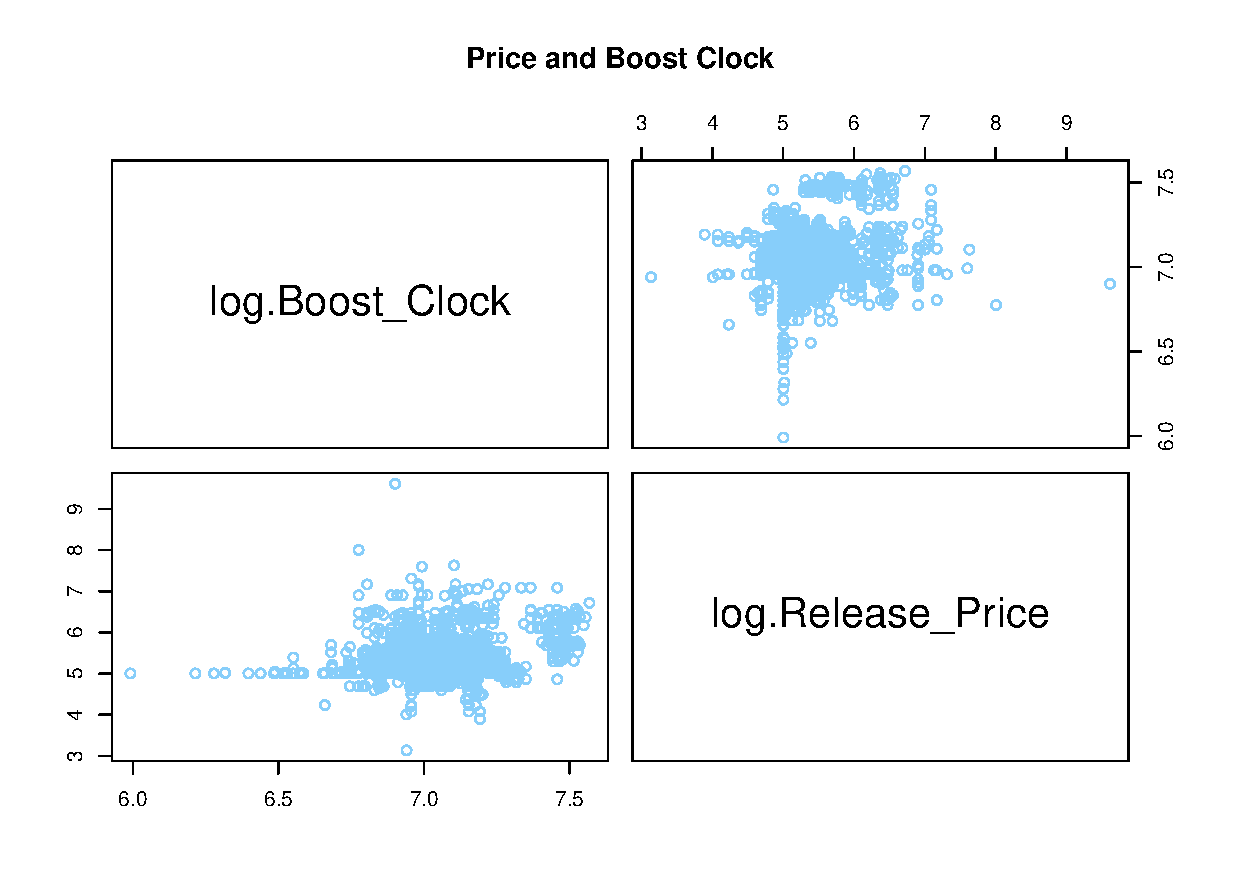
\includegraphics[keepaspectratio, width=1\textwidth, height=1\textheight]{Visualization/Pairs/price_boostclock.pdf}
        &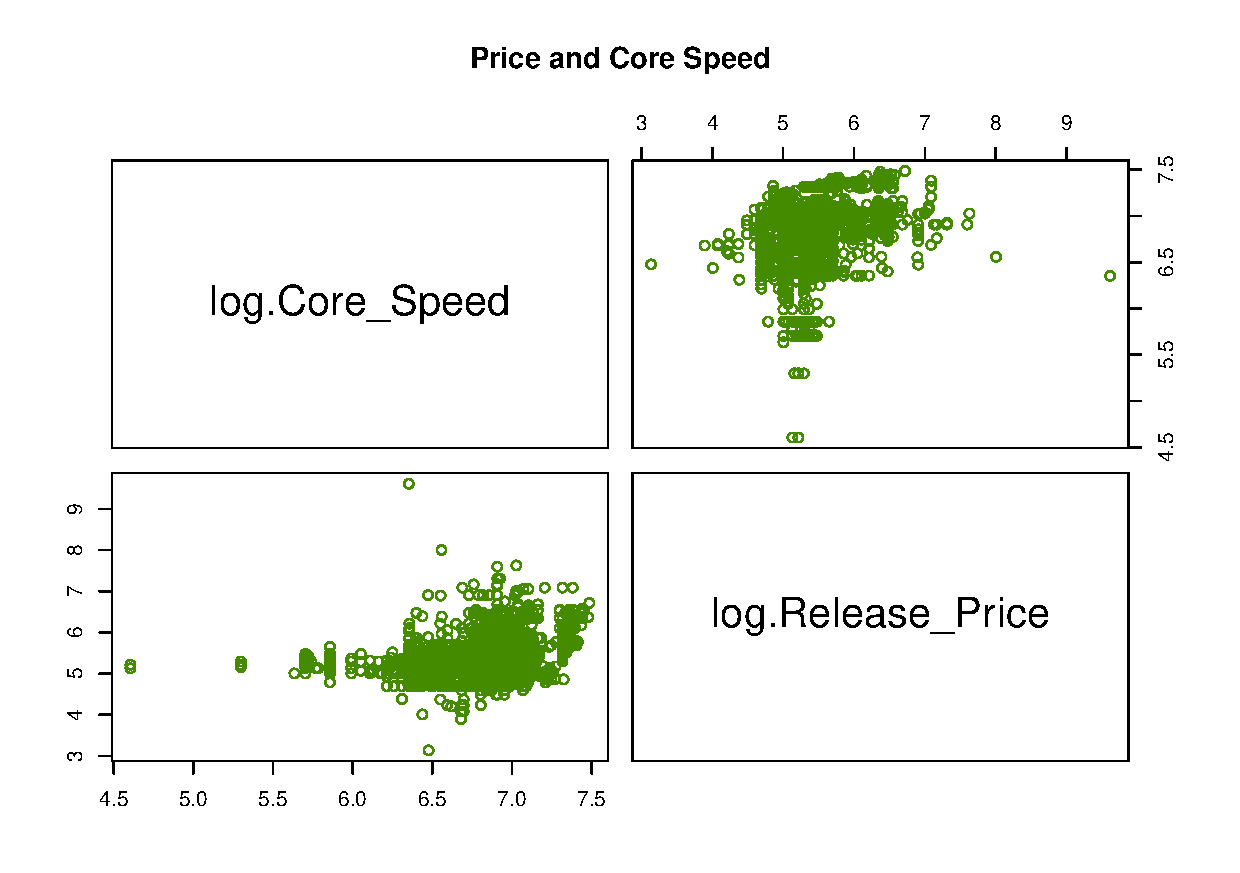
\includegraphics[keepaspectratio, width=1\textwidth, height=1\textheight]{Visualization/Pairs/price_corespeed.pdf}\\
        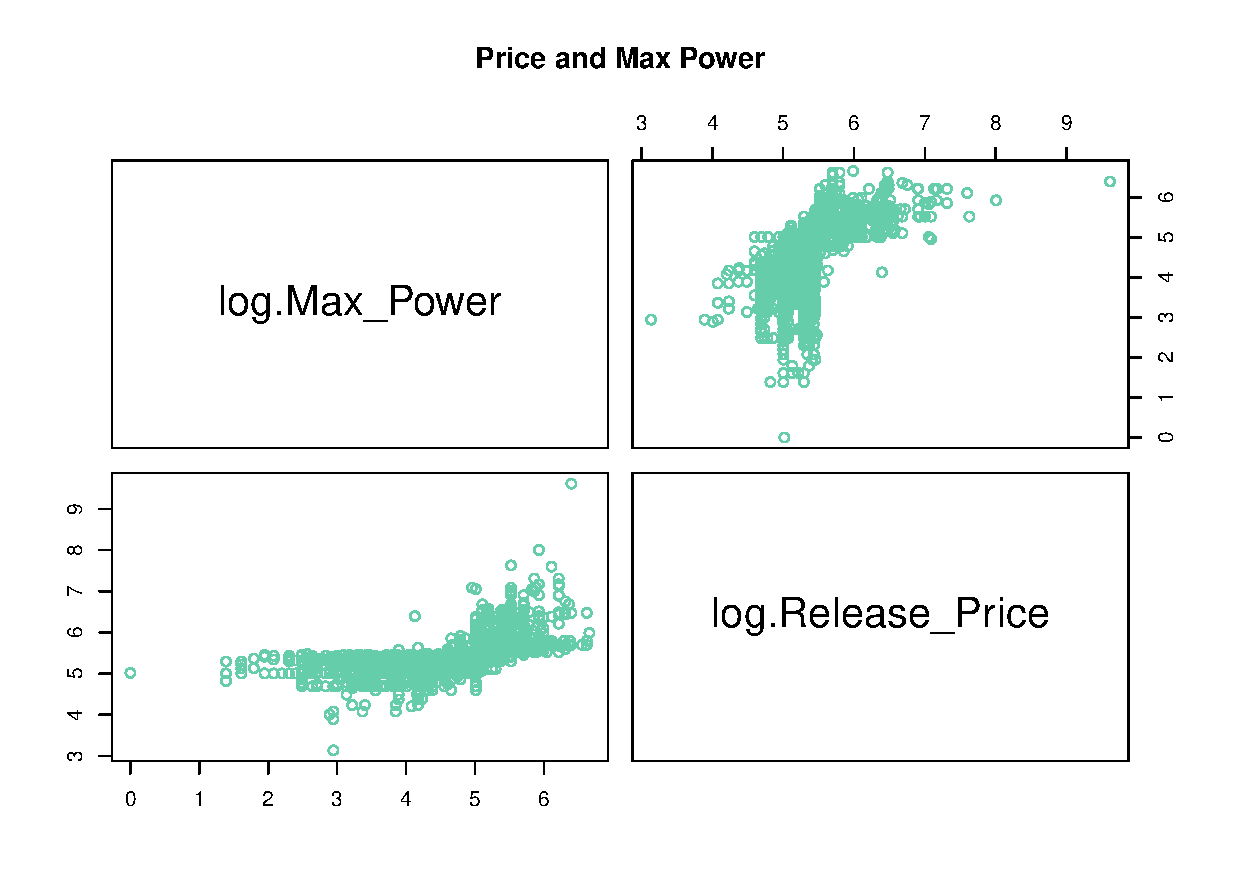
\includegraphics[keepaspectratio, width=1\textwidth, height=1\textheight]{Visualization/Pairs/price_maxpower.pdf}
        &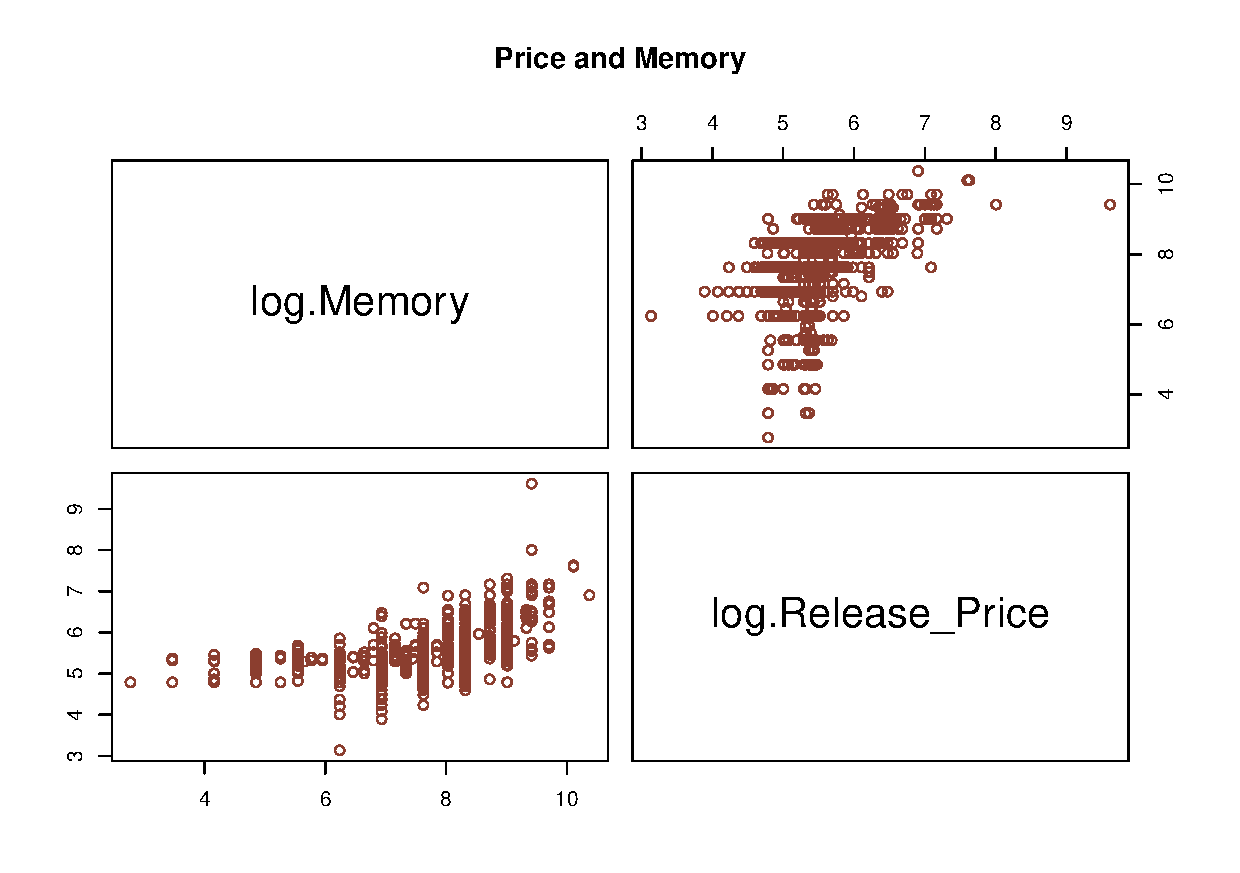
\includegraphics[keepaspectratio, width=1\textwidth, height=1\textheight]{Visualization/Pairs/price_memory.pdf}\\
        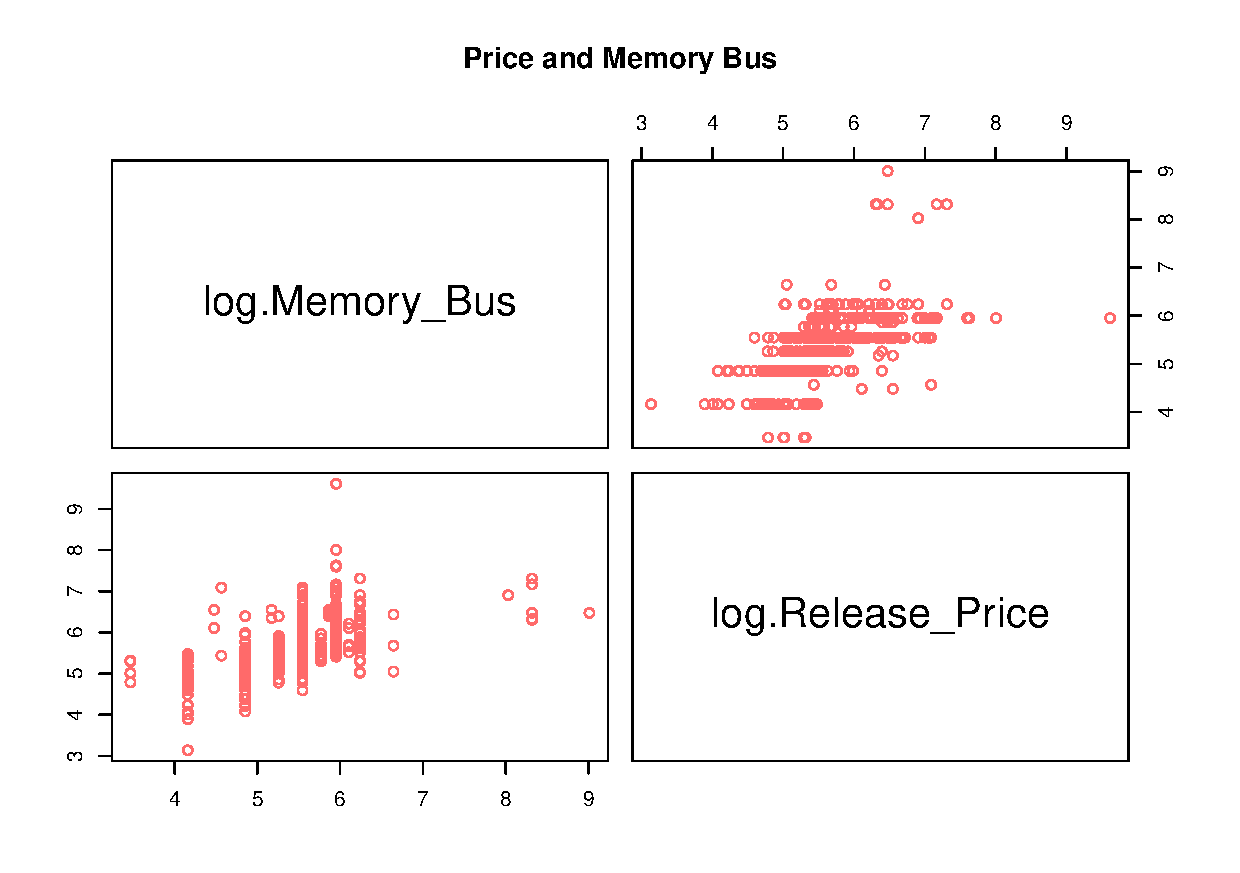
\includegraphics[keepaspectratio, width=1\textwidth, height=1\textheight]{Visualization/Pairs/price_memorybus.pdf}
        &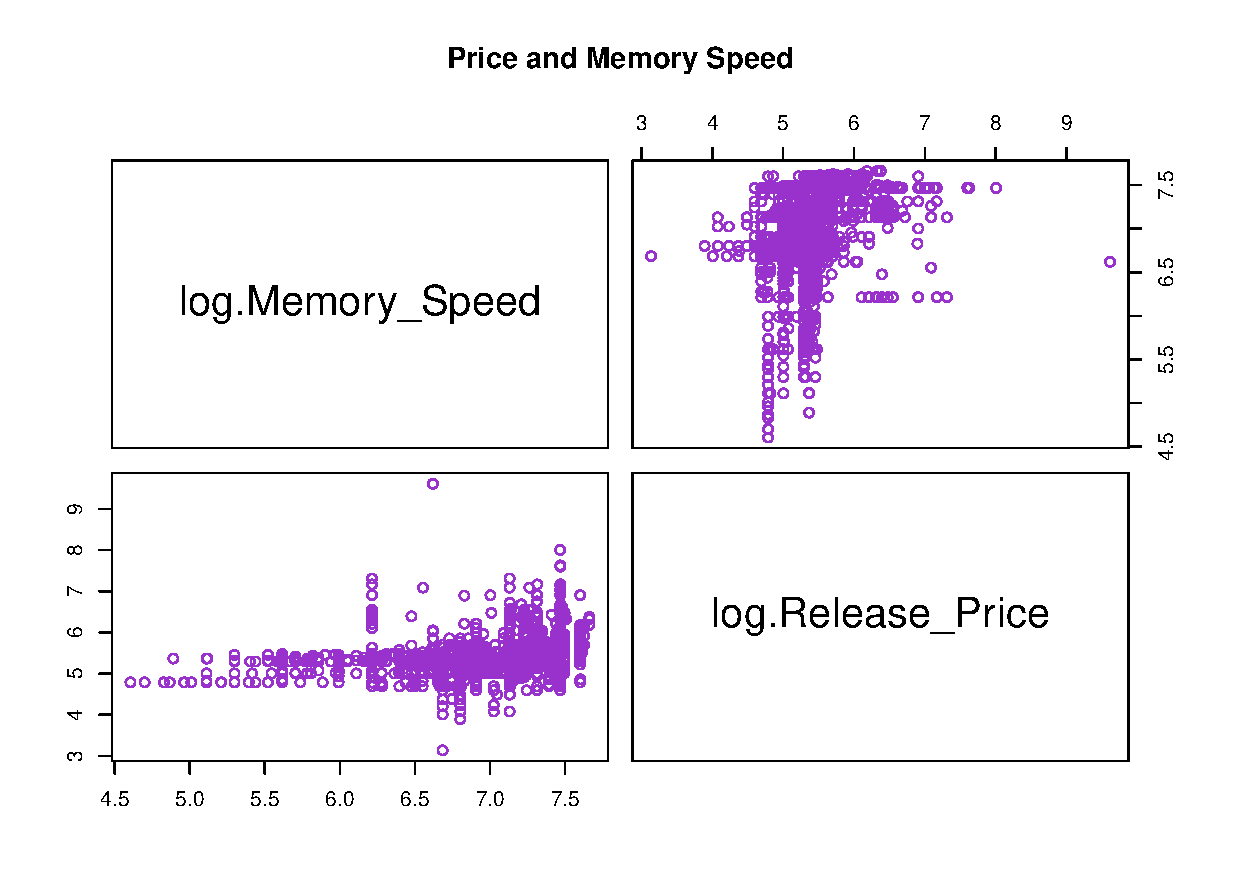
\includegraphics[keepaspectratio, width=1\textwidth, height=1\textheight]{Visualization/Pairs/price_memoryspeed.pdf}\\
        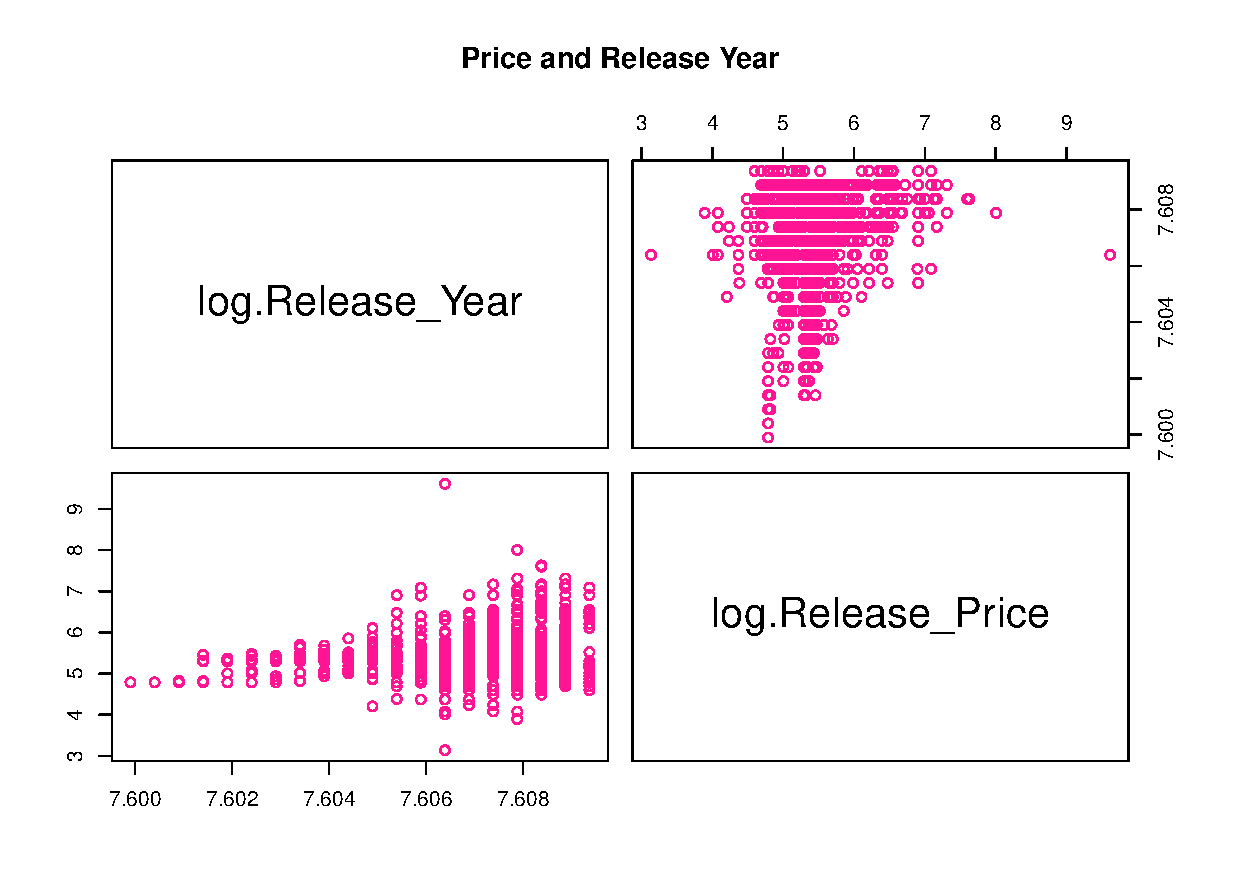
\includegraphics[keepaspectratio, width=1\textwidth, height=1\textheight]{Visualization/Pairs/price_releaseyear.pdf}
        &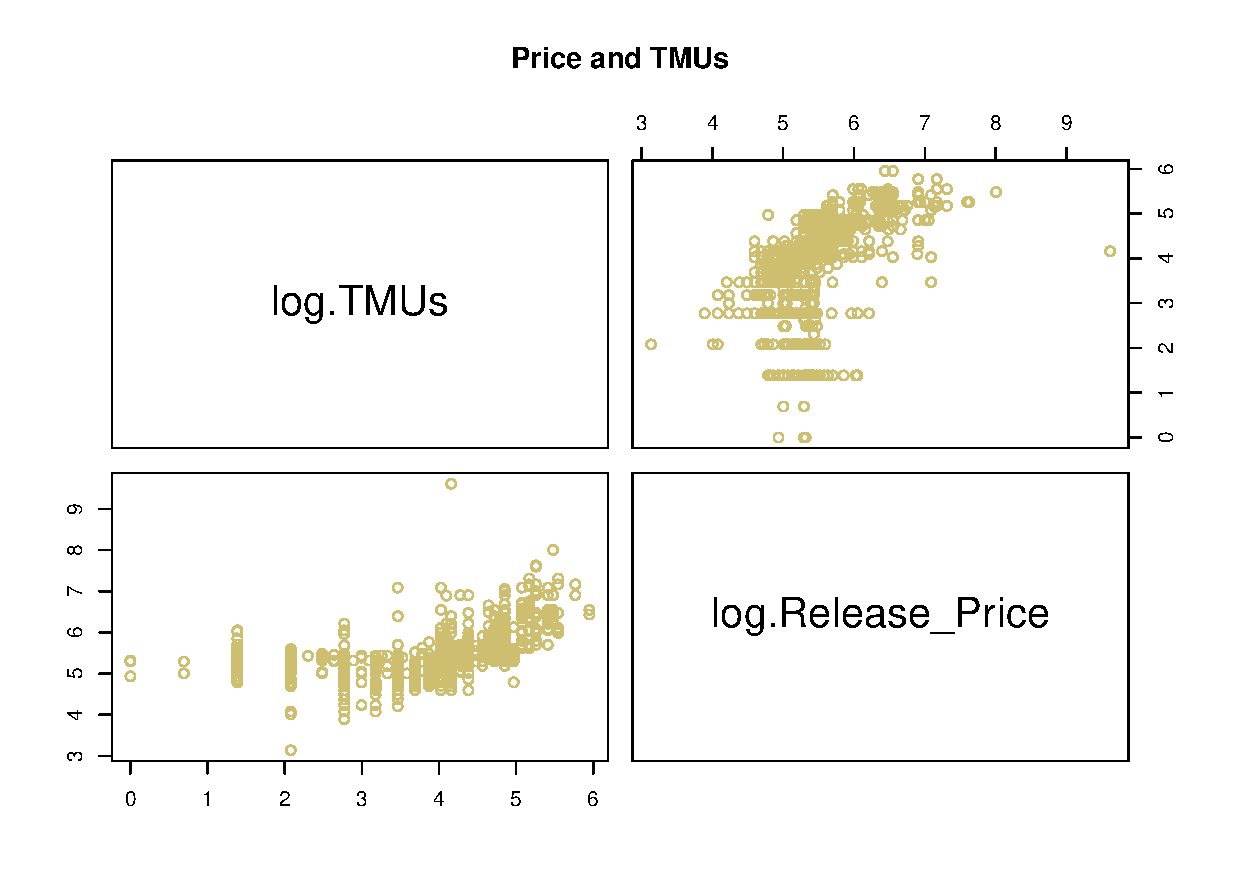
\includegraphics[keepaspectratio, width=1\textwidth, height=1\textheight]{Visualization/Pairs/price_TMUs.pdf}
    \end{tabular}
\end{adjustbox}
\end{center}
Now we try combinations of 3 or more variables.
\begin{mdframed}[leftline=false,rightline=false,backgroundcolor=lightblue!10,nobreak=false]
    \begin{minted}[linenos,breaklines,breaksymbolleft=,obeytabs=true,tabsize=2]{R}
pairs(df[,c('log.Memory','log.Memory_Bus', 'log.Memory_Speed', 'log.Release_Price')], main = "Pairs plot of Memory and Price", col = "steelblue3")
pairs(df[,c('log.Boost_Clock','log.Core_Speed','log.Max_Power', 'log.Release_Price')], main = "Pairs plot of Speed/Power and Price", col = "steelblue3")
pairs(df[,c('log.Shader','log.TMUs', 'log.Release_Price')], main = "Pairs plot of Rendering Unit and Price", col = "steelblue3")
    \end{minted}
\end{mdframed}
\begin{figure}[H]
    \centering
    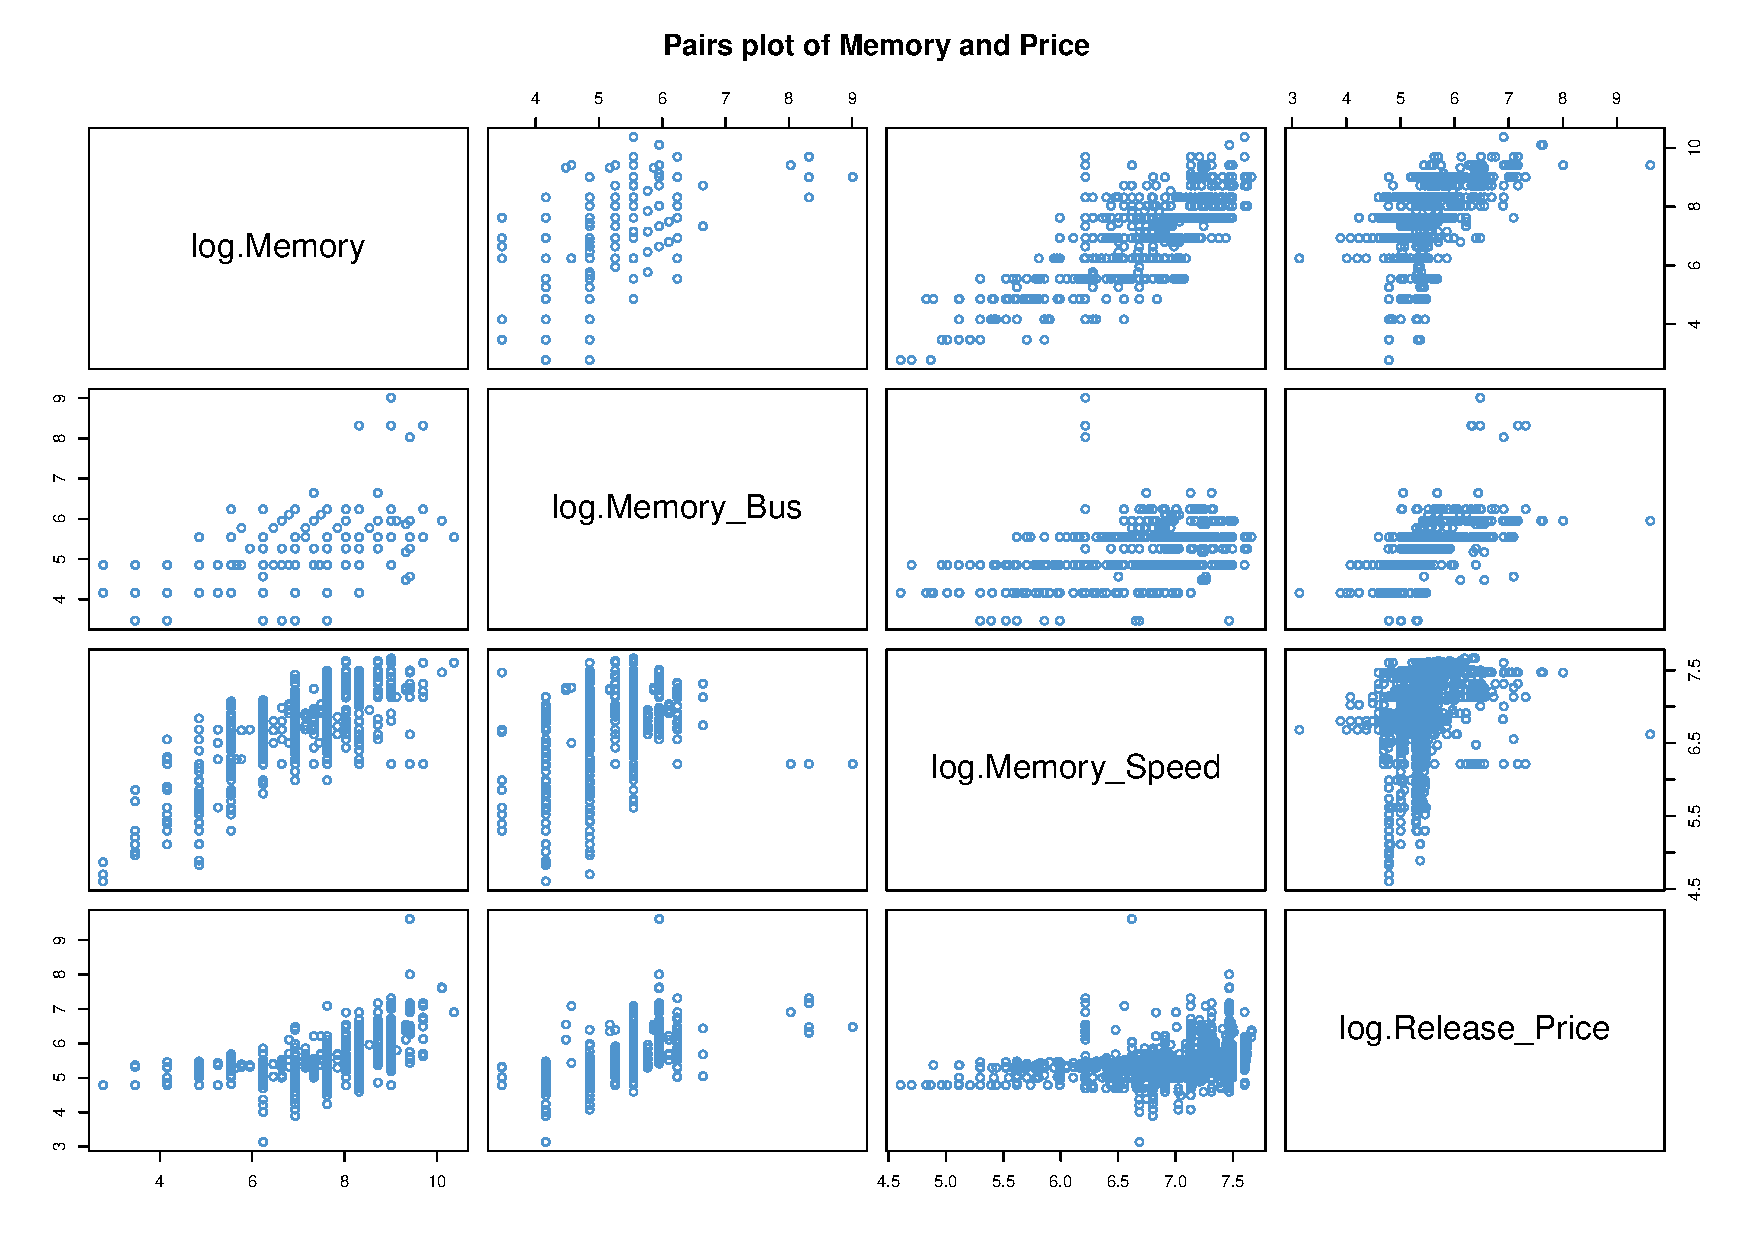
\includegraphics[keepaspectratio, width=1\textwidth, height=1\textheight]{Visualization/Pairs/mem_price.pdf}
\end{figure}
\begin{figure}[H]
    \centering
    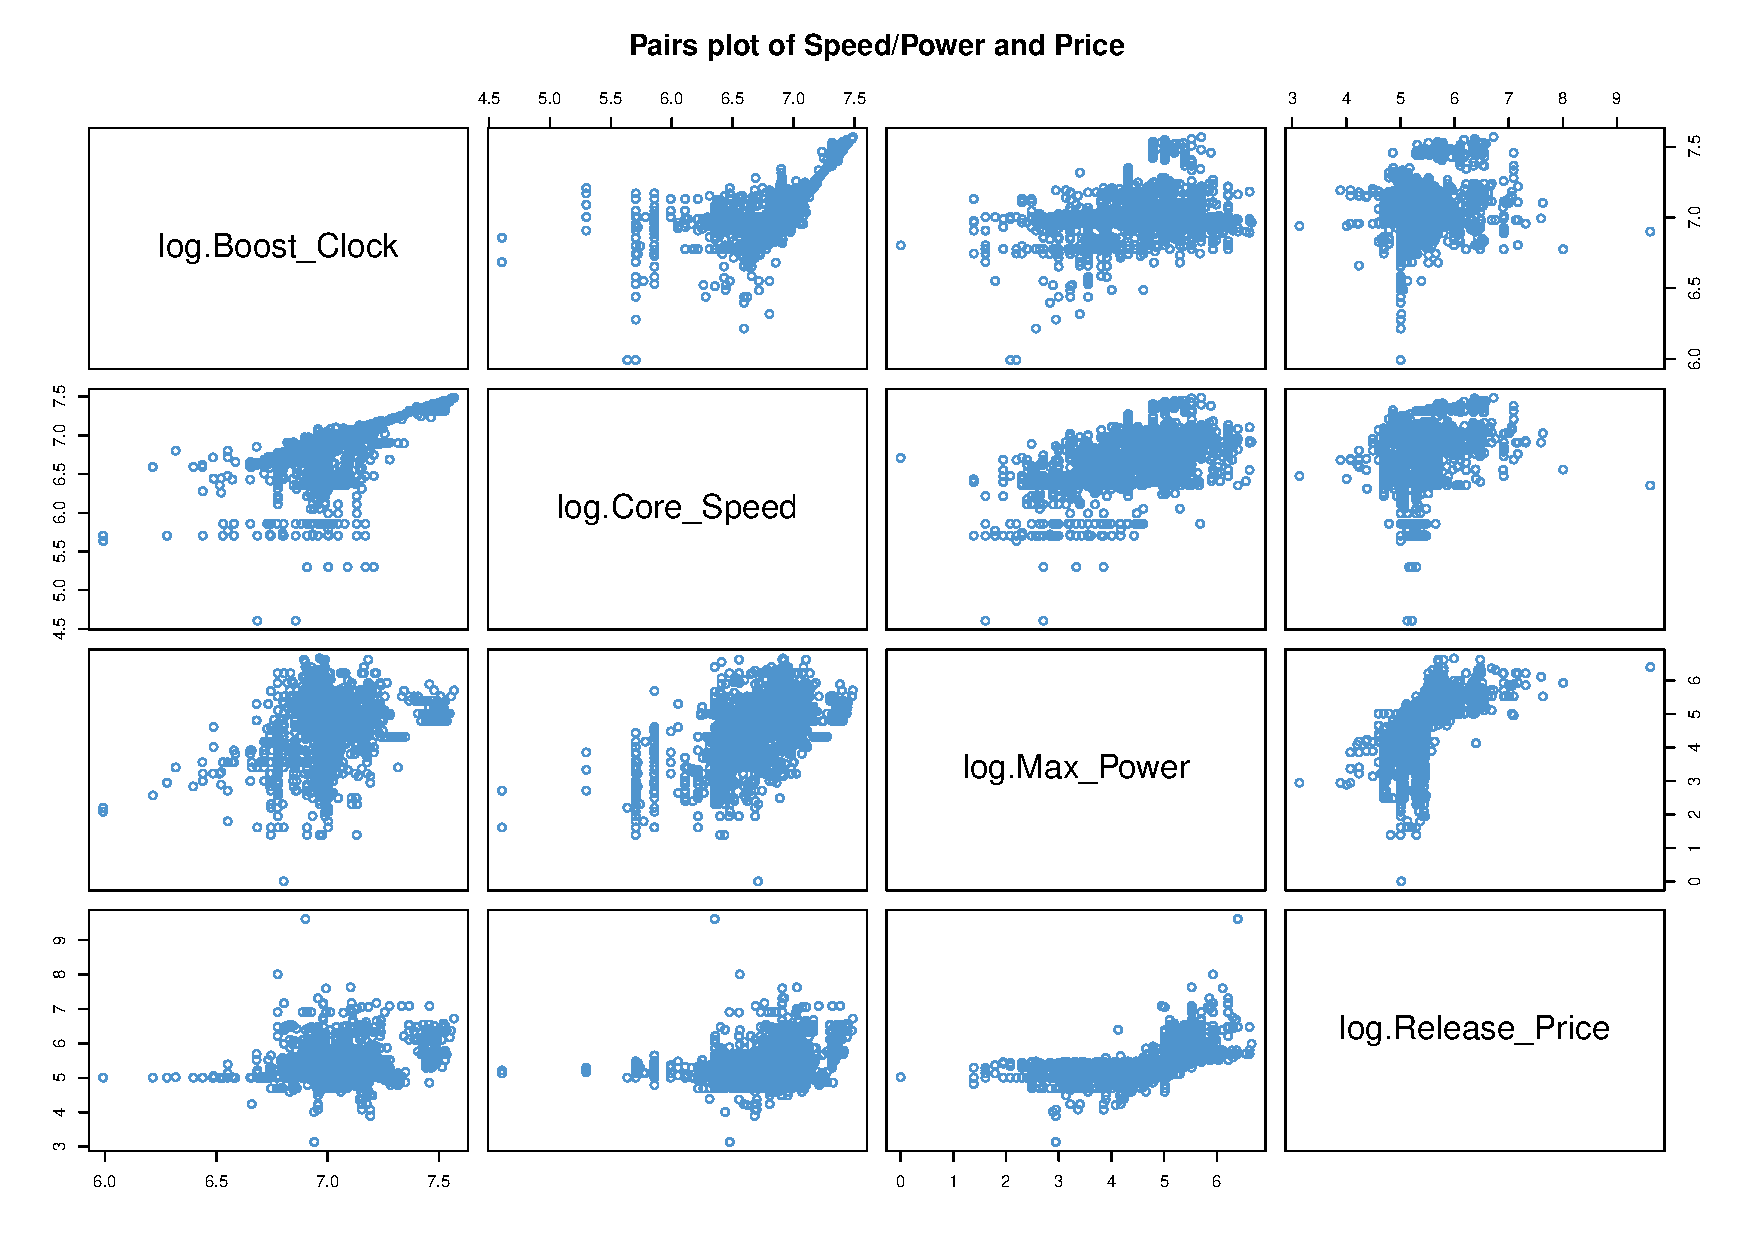
\includegraphics[keepaspectratio, width=0.9\textwidth, height=1\textheight]{Visualization/Pairs/speed_power_price.pdf}
\end{figure}
\begin{figure}[H]
    \centering
    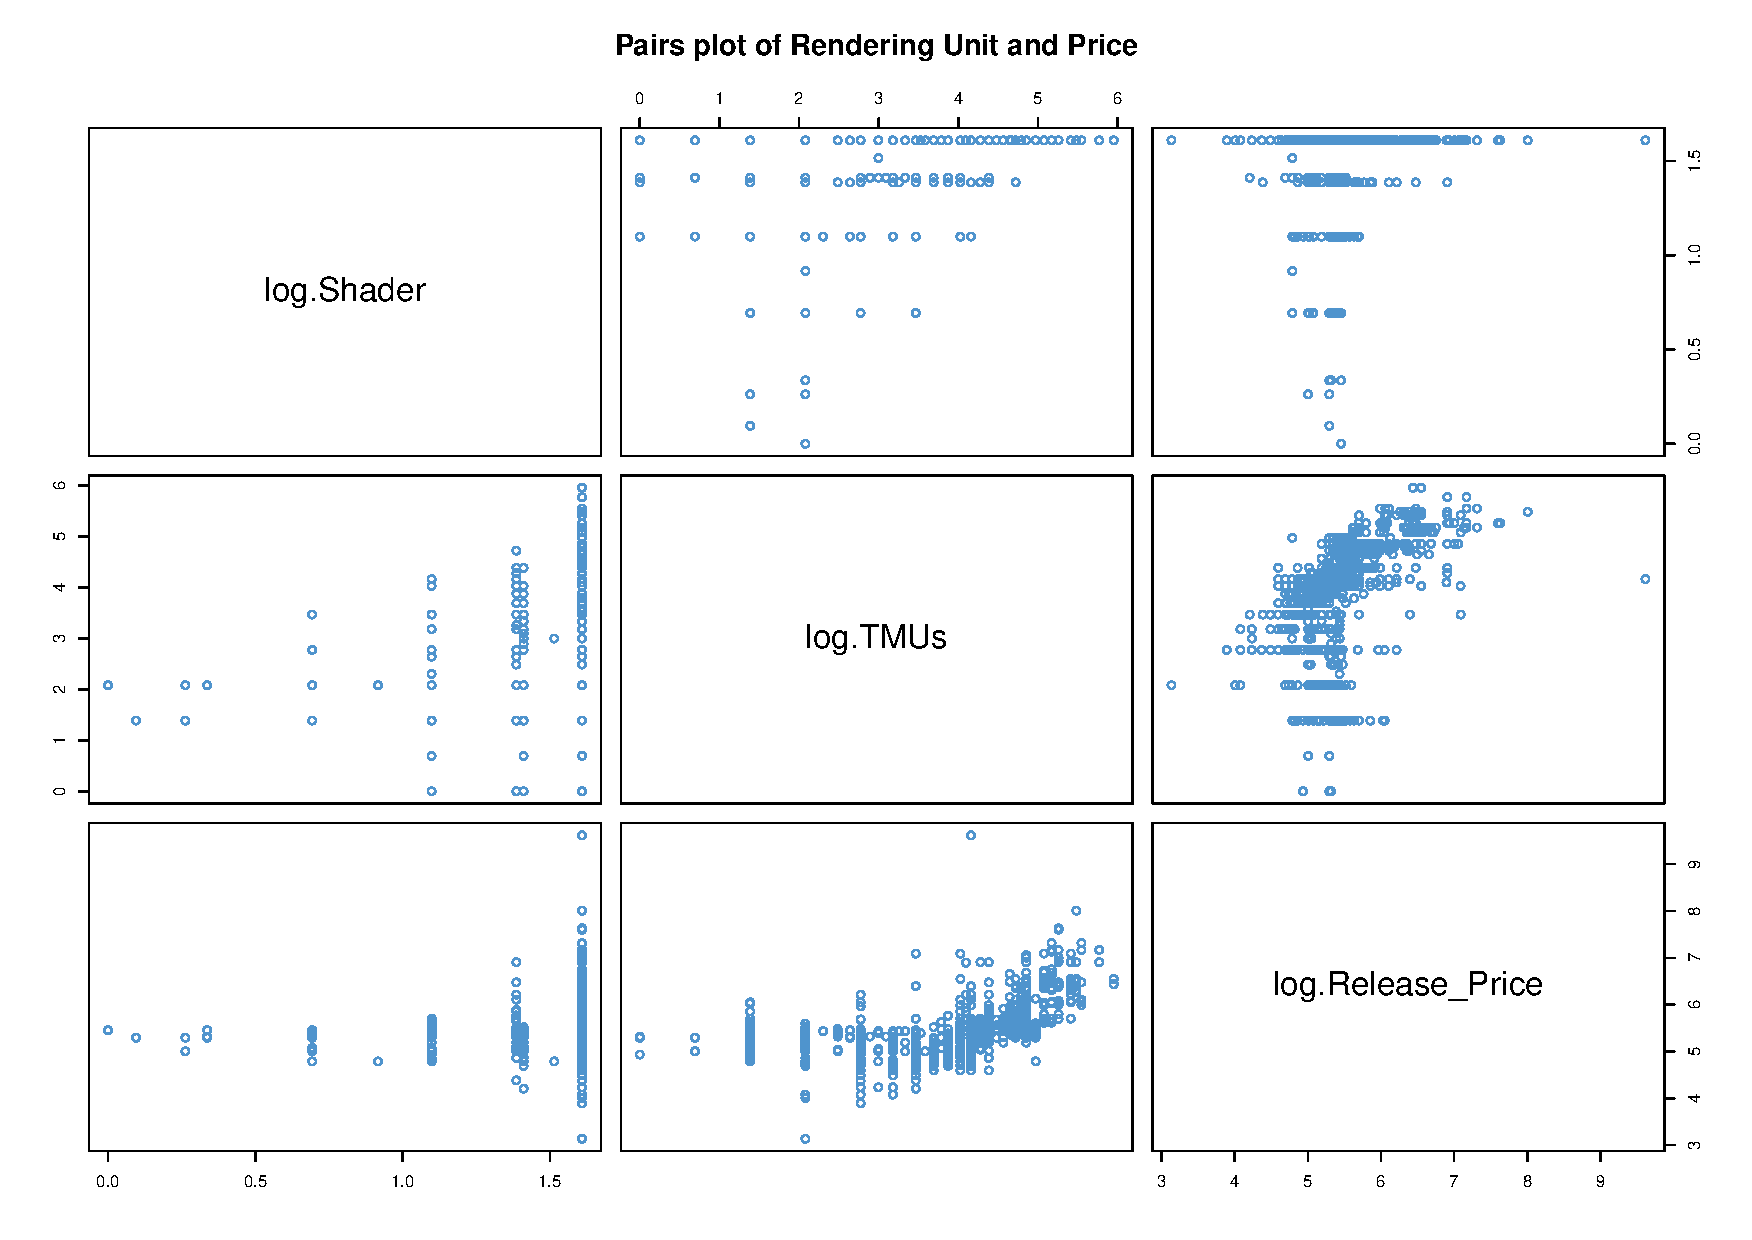
\includegraphics[keepaspectratio, width=0.9\textwidth, height=1\textheight]{Visualization/Pairs/rendering_price.pdf}
\end{figure}




%%%%%%%%%%%%%%%%%%%%%%%%%%%%%%%%%%%%%%%%%%%%%%%%%%%%%%%%%%%%%%%%%%
\section{Hypothesis testing}
A statistical hypothesis is a hypothesis that is testable on the basis of observed data modelled as the realised values taken by a collection of random variables. Hypothesis testing is a form of statistical inference that uses data from a sample to draw conclusions about a population parameter or a population probability distribution.

\subsection{ANOVA}
Analysis of variance (ANOVA) is an analysis tool used in statistics that splits an observed aggregate variability found inside a data set into two parts:
\begin{itemize}
    \item Systematic factors.
    \item Random factors
\end{itemize}
The systematic factors have a statistical influence on the data set, while the random factors do not. Analysts use the ANOVA test to determine the influence that independent variables have on the dependent variable in a regression study.
\subsubsection{One-way ANOVA}
\subsubsubsection{Basic concept}
A one-way ANOVA compares three or over three categorical groups to establish whether there is a difference between them. Within each group, there should be three or more observations, and the means of the samples are compared.\\\\
In this part, we want to know whether or not a significant difference in the average core speed among manufacturers.\\\\
First, we are going to use function selection to filter the data base on the core speed of each manufacturer in \verb|df|:
\begin{mdframed}[leftline=false,rightline=false,backgroundcolor=lightblue!10,nobreak=false]
    \begin{minted}[linenos,breaklines,breaksymbolleft=,obeytabs=true,tabsize=2]{R}
aovCore_Speed <- select(df, Manufacturer, log.Core_Speed)
    \end{minted}
\end{mdframed}
To compute one-way ANOVA test, the data in \verb|df| must be a fixed-impact model meet the follow requirements:
\begin{itemize}
\item All data are independent and collected randomly.
\item The population from those samples should be normally distributed.
\item Homogeneity of variance: the variance among the groups should be approximately equal.
\end{itemize}
\textbf{Condition 1}:\\
The data is collected based on 4 different manufacturers, so the data satisfies the first condition.\bigskip\\
\textbf{Condition 2}:\\
Normally, we will use the Shapiro-Wilk test, which is the most powerful normality test. However, due to the large sample size of the data, over 3300 GPUs satisfied after filtered, the Shapiro-Wilk test can not be used in R. Instead, we will use QQ-plot to see if the data is normally distributed \cite{bib11}:
\begin{mdframed}[leftline=false,rightline=false,backgroundcolor=lightblue!10,nobreak=false]
    \begin{minted}[linenos,breaklines,breaksymbolleft=,obeytabs=true,tabsize=2]{R}
ggqqplot(aovCore_Speed$log.Core_Speed)
    \end{minted}
\end{mdframed}
\begin{figure}[H]
    \centering
    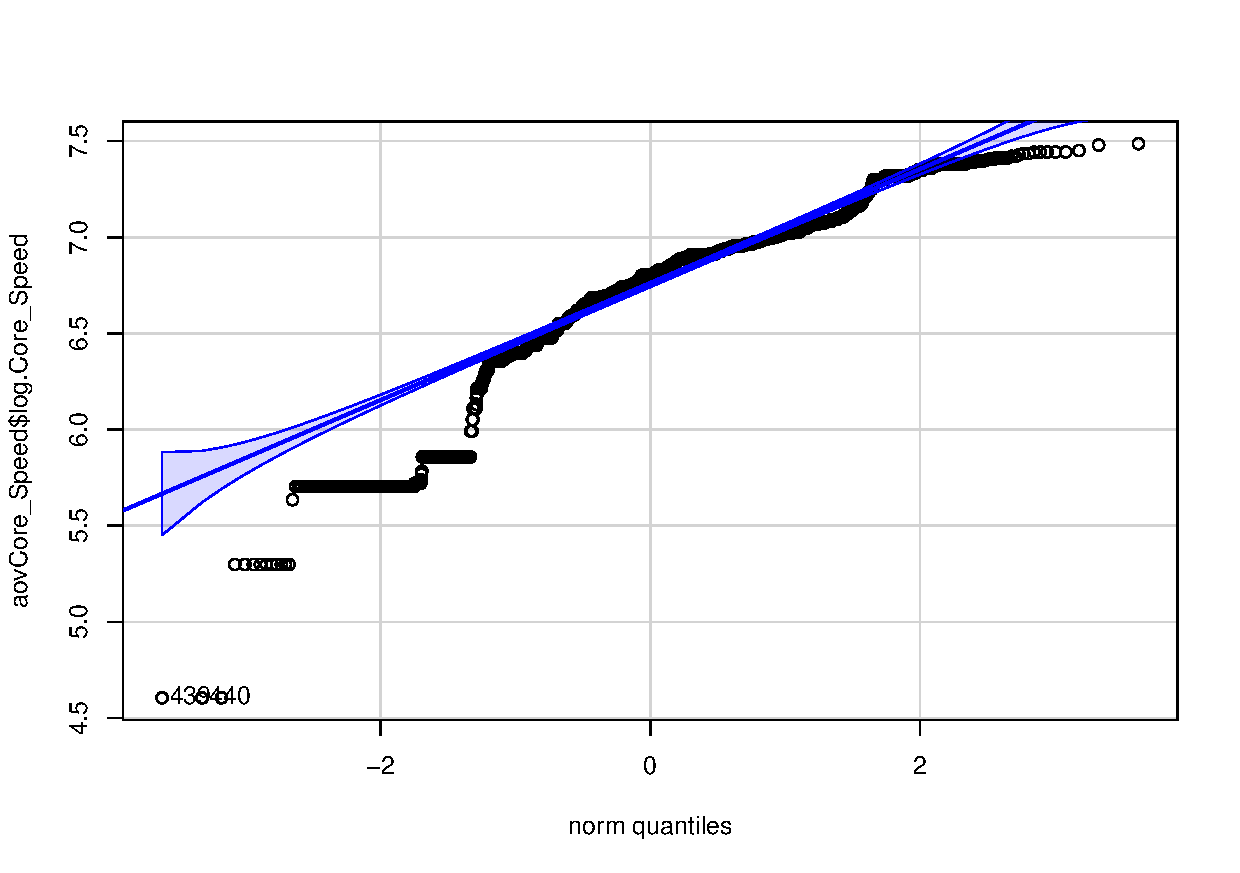
\includegraphics[keepaspectratio, width=1\textwidth, height=1\textheight]{Hypothesis/ANOVA/QQ_Plot.pdf}
\end{figure}
In theory, sampled data from a normal distribution would fall along the dotted line. In reality, even data sampled from a normal distribution can exhibit some deviation from the line.\bigskip \\
According to the plot above, the data are not normally distributed. Nonetheless the sample size is sufficiently large ($>200$), the normality assumption is not needed at all as the Central Limit Theorem ensures that the distribution of disturbance term will approximate normality. Also, the one-way ANOVA is considered a robust test against the normality assumption. This means that it tolerates violations to its normality assumption rather well. As regards the normality of group data, the one-way ANOVA can tolerate data that is non-normal (skewed) with only a small effect on the Type I error rate.\bigskip\\
We can conclude that the second condition is not necessarily satisfied.

\subsubsubsection{Building test}
If we assume that, the data is homogeneous, which means it satisfies the one-way ANOVA assumptions. We will do the one-way ANOVA in R through these steps below:\bigskip\\
\textbf{Step 1}: In order to determine if there is any significant difference in core speed among these manufacturers, we enumerate the null hypothesis $H_0$ and alternative hypothesis $H_1$.
\begin{itemize}
    \item $H_0: u_1=u_2=...=u_i=0$: There is a similarity in average core speed among 4 manufacturers: Nvidia, AMD, Intel and ATI.
    \item $H_1: u_i \neq 0$ for at least one $i$ .At least one of the manufacturer have a significant different in average \verb|Core_Speed| compared to others.
\end{itemize}
We let $\alpha$ (significant level) = 0.05 by default.\bigskip\\
\textbf{Step 2}: Select the appropriate test statistic.\\
We choose one-way ANOVA to compare 4 means in this hypothesis test.\\
The formula for the test statistic is:
\begin{equation*}
F=\dfrac{MSTr}{MSE}=\dfrac{\dfrac{SSTr}{a-1}}{\dfrac{SSE}{a(n-1)}}
\end{equation*}
where:
\begin{itemize}
    \item $MSTr$ is mean square for treatments.
    \item $MSE$ is mean square for error.
    \item $SSTr$ is treatment sum of squares.
    \item $SSE$ is error sum of squares.
    \item $a$ is number of treatments.
    \item $n$ is number of observations of each treatment (number of sample collected for each treatment).
\end{itemize}
\bigskip
\textbf{Step 3}:  We will calculate the $SSTr$ with degree of freedom $a - 1$ and $SSE$ with degree of freedom $a(n-1)$ using the data from the provided table and the following formula:

\begin{align*}
    SST &= \sum_{i=1}^I \sum_{j=1}^{J_i} y^2_{ij}-\dfrac{y^2..}{n}\\
    SSTr &= \sum_{i=1}^a \dfrac{y^2_i.}{n}-\dfrac{y^2..}{N}\\
    SSE &= SST - SSTr
\end{align*}
where:
\begin{itemize}
    \item $SST$ is the total sum of squares.
    \item $i$ is the index of treatment.
    \item $j$ is the index of observation(samples).
    \item $y_{ij}$ is the data of the table at $i$ treatments and $j$ observations.
    \item $y_i.$ is the total sum of observations(samples) for $i$ treatment.
    \item $y..$ is the total sum of $y_1+y_2+...+y_a$.
\end{itemize}
\bigskip
\textbf{Step 4}: Compute the test statistic.\\
We use RStudio to analysis with the filtered data to fulfill the request:
\begin{mdframed}[leftline=false,rightline=false,backgroundcolor=lightblue!10,nobreak=false]
    \begin{minted}[linenos,breaklines,breaksymbolleft=,obeytabs=true,tabsize=2]{R}
aov_one <- aov(log.Core_Speed ~ Manufacturer, data = aovCore_Speed)
aov_one
summary(aov_one)
    \end{minted}
\end{mdframed}
\begin{lstlisting}
 Terms:
                 Manufacturer Residuals
 Sum of Squares      237.3332  287.2447
 Deg. of Freedom            3      3361

 Residual standard error: 0.2923424
 Estimated effects may be unbalanced

                Df Sum Sq Mean Sq F value Pr(>F)    
 Manufacturer    3  237.3   79.11   925.7 <2e-16 ***
 Residuals    3361  287.2    0.09                   
 ---
 Signif. codes:  0 '***' 0.001 '**' 0.01 '*' 0.05 '.' 0.1 ' ' 1
\end{lstlisting}
From F distribution table, we have $f_{0.05, 3, \infty} = 2.2141$ , therefore, $f_0 > f_{0.05,3,\infty}$ , we can reject the null hypothesis $H_0$.\\\\
Before we go to the final conclusion, we check the third condition.\\\\
\textbf{Condition 3}:\\
As we have condition 2 is satisfied, we will use Levene-test to evaluate if the variances of two populations are equal. In statistics, Levene’s test is an inferential statistic used to evaluate the equality of variances for a variable determined by two or more groups. For Levene’s test the statistical hypotheses are:
\begin{itemize}
    \item Null hypothesis $H_0$: All populations are equal.
    \item Alternative hypothesis $H_1$: At least two of them differ.
\end{itemize}
Thus, if the p-value is larger than the chosen $\alpha$ level, then the null hypothesis $H_0$ is not rejected and there is evidence that the variances of two populations are equal.\\\\
We use RStudio to perform Levene-test on the dataset:
\begin{mdframed}[leftline=false,rightline=false,backgroundcolor=lightblue!10,nobreak=false]
    \begin{minted}[linenos,breaklines,breaksymbolleft=,obeytabs=true,tabsize=2]{R}
leveneTest(log.Core_Speed ~ Manufacturer, aovCore_Speed, center = mean)
    \end{minted}
\end{mdframed}
\begin{lstlisting}
 Levene's Test for Homogeneity of Variance (center = mean)
         Df F value    Pr(>F)    
 group    3   42.09  <2.2e-16 ***
       3361                      
 ---
 Signif. codes:  0 '***' 0.001 '**' 0.01 '*' 0.05 '.' 0.1 ' ' 1
\end{lstlisting}
From the output above, we can see that the p-value \verb|(< 2.2e-16)| is much smaller compares to the alpha level 0.05. Now we reject the null hypothesis $H_0$ that all populations are equal, which also means there is a difference among manufacturers.
\subsubsubsection{Welch’s test}
Because of the condition 3 above is not satisfied for the one-way ANOVA, we will use the Welch’s test instead. Welch’s Test for Unequal Variances (also called Welch’s t test, Welch’s adjusted T or unequal variances t-test) is a modification of Student’s t-test(more reliable when the two samples have unequal variances and/or unequal sample sizes) to see if two sample means are significantly different. The modification is to the degrees of freedom used in the test, which increases the test power for samples with unequal variance. There are two hypotheses in the Welch’s test:

\begin{itemize}
    \item Null hypothesis $H_0$: for the test is that the means are equal.
    \item Alternative hypothesis $H_1$: for the test is that means are not equal.
\end{itemize}
Below is the formula of Welch’s test:
\begin{equation*}
    t = \dfrac{\overline{X_1}-\overline{X_2}}{\sqrt{\dfrac{s^2_1}{n_1}+\dfrac{s^2_2}{n_2}}}=\dfrac{\overline{X_1}-\overline{X_2}}{\sqrt{se^2_1+se^2_2}}
\end{equation*}
where:
\begin{itemize}
    \item $\overline{X_i}$ is the $i^{th}$ sample mean.
    \item $s_i$ is the $i^{th}$ standard deviation.
\end{itemize}
Now we perform the Welch’s test in R:
\begin{mdframed}[leftline=false,rightline=false,backgroundcolor=lightblue!10,nobreak=false]
    \begin{minted}[linenos,breaklines,breaksymbolleft=,obeytabs=true,tabsize=2]{R}
oneway.test(log.Core_Speed ~ Manufacturer, data=aovCore_Speed)
    \end{minted}
\end{mdframed}
\begin{lstlisting}
 One-way analysis of means (not assuming equal variances)

 data:  log.Core_Speed and Manufacturer
 F = 1301.5, num df = 3.00, denom df = 488.59, p-value < 2.2e-16
\end{lstlisting}
\bigskip
\textbf{Conclusion}:
According to the one-way ANOVA test and the Welch’s test, which also results in rejecting the null
hypothesis due to the p-value, we can officially claim that there is a difference in average core speed among manufacturers.

\subsubsection{Two-way ANOVA}
\subsubsubsection{Basic concept}
A two-way ANOVA is designed to assess the interrelationship of two independent variables on a dependent variable. A two-way ANOVA is an extension of the one-way ANOVA. Use two-way ANOVA when there is one measure variable (i.e. a quantitative variable) and two nominal variables \cite{bib9}.\\\\
A two-way ANOVA with interaction tests three null hypotheses at the same time:
\begin{itemize}
    \item There is no difference in group means at any level of the first independent variable.
    \item There is no difference in group means at any level of the second independent variable.
    \item The effect of one independent variable does not depend on the effect of the other independent variable (a.k.a. no interaction effect).
\end{itemize}
Note that a two-way ANOVA without interaction (a.k.a. an additive two-way ANOVA) only tests the first two of these hypotheses. And it is almost as if the dataset that we chose just allows us to do that.
We assume that there are 3 price segments for GPUs (based on \verb|Release_Price|):
\begin{itemize}
    \item Bugdet: Under \$200.
    \item Midrange: From \$200 to \$600.
    \item Highend: Above \$600.
\end{itemize}
In this part, our hypothesis is:
\begin{itemize}
    \item $H_0$: There is no difference in average core speed for any GPU manufacturer and in all 3 price segments.
    \item $H_1$: There is a difference in average core speed for any GPU manufacturer and in all 3 price segments.
\end{itemize}
We create a variable \verb|Label| and assign a value to this variable based on the GPU price.
\begin{mdframed}[leftline=false,rightline=false,backgroundcolor=lightblue!10,nobreak=false]
    \begin{minted}[linenos,breaklines,breaksymbolleft=,obeytabs=true,tabsize=2]{R}
df$Label <- cut(df$log.Release_Price, c(log(0), log(200), log(600), log(15000)), labels=c("Budget", "Midrange", "Highend"), include.lowest=T)
    \end{minted}
\end{mdframed}
As a result, we have 2 nominal quantities and 1 quantitative quantity:
\begin{itemize}
    \item \verb|Manufacturer|: AMD, ATI, Intel and Nvidia.
    \item \verb|Label|: Budget, Midrange and Highend.
    \item \verb|log.Release_Price|: Price of GPU.
\end{itemize}
Two-way ANOVA requires a few assumptions:
\begin{enumerate}
    \item Homogeneity of variance (a.k.a. homoscedasticity).
    \item Independence of observations.
    \item Normally-distributed dependent variable.
\end{enumerate}
In our data set, the response variable is normally distributed, and we can check for homoscedasticity in the back.
\subsubsubsection{Building test}
Now we will implement the two-way ANOVA model in R:
\begin{mdframed}[leftline=false,rightline=false,backgroundcolor=lightblue!10,nobreak=false]
    \begin{minted}[linenos,breaklines,breaksymbolleft=,obeytabs=true,tabsize=2]{R}
aov_two <- aov(log.Core_Speed ~ Manufacturer + Label, data = df)
aov_two
summary(aov_two)
    \end{minted}
\end{mdframed}
\begin{lstlisting}
 Call:
    aov(formula = log.Core_Speed ~ Manufacturer + Label, data = df)

 Terms:
                 Manufacturer     Label Residuals
 Sum of Squares     237.33325  16.15822 271.08648
 Deg. of Freedom            3         2      3359

 Residual standard error: 0.2840854
 
 Estimated effects may be unbalanced
                Df Sum Sq Mean Sq F value Pr(>F)    
 Manufacturer    3 237.33   79.11   980.3 <2e-16 ***
 Label           2  16.16    8.08   100.1 <2e-16 ***
 Residuals    3359 271.09    0.08                   
 ---
 Signif. codes:  0 '***' 0.001 '**' 0.01 '*' 0.05 '.' 0.1 ' ' 1
\end{lstlisting}
From the result above, we can see that both manufacturer type and price segment explain a significant amount of variation in average core speed (p-value $<$ 0.001).
\subsubsubsection{Post hoc test}
ANOVA will tell us which parameters are significant, but not which levels are actually different from one another. To test this we can use a post-hoc test. The Tukey’s Honestly-Significant-Difference (TukeyHSD) test lets us see which groups are different from one another.
\begin{mdframed}[leftline=false,rightline=false,backgroundcolor=lightblue!10,nobreak=false]
    \begin{minted}[linenos,breaklines,breaksymbolleft=,obeytabs=true,tabsize=2]{R}
TukeyHSD(aov_two)
    \end{minted}
\end{mdframed}
\begin{lstlisting}
 Tukey multiple comparisons of means
     95% family-wise confidence level

 Fit: aov(formula = log.Core_Speed ~ Manufacturer + Label, data = df)

 $Manufacturer
                    diff         lwr         upr    p adj
 ATI-AMD       0.2734123  0.19257382  0.35425076 0.00e+00
 Intel-AMD    -0.8968407 -0.94689573 -0.84678563 0.00e+00
 Nvidia-AMD    0.1245477  0.09775552  0.15133986 0.00e+00
 Intel-ATI    -1.1702530 -1.26095908 -1.07954687 0.00e+00
 Nvidia-ATI   -0.1488646 -0.22911364 -0.06861555 1.15e-05
 Nvidia-Intel  1.0213884  0.97229094  1.07048581 0.00e+00

 $Label
                       diff        lwr       upr p adj
 Midrange-Budget  0.1098742 0.08648174 0.1332667     0
 Highend-Budget   0.2857955 0.22056322 0.3510278     0
 Highend-Midrange 0.1759213 0.11044972 0.2413929     0
\end{lstlisting}
\textbf{Conclusion}: This output shows the pairwise differences between the four types of \verb|Manufacturer| and between the three levels of \verb|Label|, with the average difference (\verb|diff|), the lower and upper bounds of the 95\% confidence interval (\verb|lwr| and \verb|upr|) and the p-value of the difference (\verb|p-adj|).
From the post-hoc test results, we see that there are significant differences (p $<$ 0.05) between all groups. That is, there is a statistically significant interaction between the effects of manufacturer and price segment on the starting price.

\subsection{Z-test}
One of the most common hypothesis testing method in statistics is the Z-test, used to determine whether the means of two groups are equal to each other. Note that while the T-test and Z-test have quite similar formulas, the selection of a particular test relies on sample size and the standard deviation of population. More specifically, we use the T-test when the sample size is less than 30 units, and Z-test is practically conducted when its size crosses the 30 units.\\\\
Because the dataset has a large sample size (the number of observations is more than 3000), we choose the Z-test instead of the T-test.\\\\
For the difference between Z-test and ANOVA:
\begin{itemize}
    \item Z-test assesses whether mean of two groups are statistically different from each other or not.
    \item ANOVA assesses whether the average of more than two groups is statistically different.
\end{itemize}
\subsubsection{One-sample Z-test}
\subsubsubsection{Basic concept}
A one-sample Z test is one of the most basic types of hypothesis test. It is used when we want to know whether the difference between the mean of a sample mean and the mean of a population is large enough to be statistically significant. \\\\
Assumptions of one-sample Z hypothesis test:
\begin{itemize}
    \item Population data is continuous.
    \item Population follows a standard normal distribution.
    \item The mean and standard deviation of the population is known.
    \item Samples are independent of each other.
    \item The sample should be randomly selected from the population
\end{itemize}
\subsubsubsection{Building test}
To take an example, we want to investigate the average memory among manufactures can be larger than 3000 MB or not.
\begin{mdframed}[leftline=false,rightline=false,backgroundcolor=lightblue!10,nobreak=false]
    \begin{minted}[linenos,breaklines,breaksymbolleft=,obeytabs=true,tabsize=2]{R}
df_z_one = df %>% select('Memory')
    \end{minted}
\end{mdframed}
In order to run a one-sample Z test, we need to work through several steps:\\\\
\textbf{Step 1}: State the Null Hypothesis and the Alternative Hypothesis. The null hypothesis $H_0$ states that the sample mean is NOT different from the population mean. The alternative hypothesis, in the opposite, identify data that can disprove the null hypothesis. This is one of the common stumbling blocks–in order to make sense of the sample. 
$$H_0: \mu = \mu_0,\ \ \ H_A: \mu \neq \mu_0$$
$$H_0: \mu \leq \mu_0,\ \ \ H_A: \mu > \mu_0$$
$$H_0: \mu \geq \mu_0,\ \ \ H_A: \mu < \mu_0$$
In this project, we choose our hypothesis test as:
\begin{itemize}
    \item $H_0$: The average memory is equal or larger than 3000 MB.
    \item $H_A$: The average memory is less than 3000 MB.
\end{itemize}
\textbf{Step 2}: Specify significance level ($\alpha$). Often, we choose significance levels equal to 0.01, 0.05, or 0.10; but any value between 0 and 1 can be used. In this project, we choose $\alpha = 0.05$, which means 5\% chance of producing a significant result when the null hypothesis is correct.\\\\
\textbf{Step 3}:  Compute the test statistic. Z-statistic is defined as:
$$Z = \dfrac{\overline{x}-\mu_0}{\sigma / \sqrt{n}}$$
We will use this function to calculate Z:
\begin{mdframed}[leftline=false,rightline=false,backgroundcolor=lightblue!10,nobreak=false]
\begin{minted}[linenos,breaklines,breaksymbolleft=,obeytabs=true,tabsize=2]{R}
zStat <- (mean(df_z_one$Memory) - 3000) / (sd(df_z_one$Memory) / sqrt(nrow(df_z_one)))
print(zStat)      
\end{minted}
\end{mdframed}
\begin{lstlisting}
 -7.84571
\end{lstlisting}
\textbf{Step 4}: Find the critical value or compute corresponding probability value. This step of the hypothesis testing also involves the construction of the confidence interval depending upon the testing approach.\\\\
We use student's t-distribution and normal distribution to get the p-value:
\begin{mdframed}[leftline=false,rightline=false,backgroundcolor=lightblue!10,nobreak=false]
\begin{minted}[linenos,breaklines,breaksymbolleft=,obeytabs=true,tabsize=2]{R}
pt(zStat, nrow(df_z_one) - 1)    
\end{minted}
\end{mdframed}
\begin{lstlisting}
 2.868698e-15
\end{lstlisting}
\begin{mdframed}[leftline=false,rightline=false,backgroundcolor=lightblue!10,nobreak=false]
\begin{minted}[linenos,breaklines,breaksymbolleft=,obeytabs=true,tabsize=2]{R}
pnorm(q=zStat, lower.tail=TRUE)
\end{minted}
\end{mdframed}
\begin{lstlisting}
 2.152562e-15
\end{lstlisting}
Note that we find here 2 different numbers, since those two numbers are very small, we assume they are equal.\\\\
\textbf{Step 5}: Construct acceptance / rejection regions and draw a conclusion. At the final step, we will reject or accept (fail to reject) the null hypothesis by making comparisons the critical value with the test statistic or P-value with significance level and make a general conclusion. So with our calculation, the p-value is very small than $\alpha$, we can reject the null hypothesis. To sum up here, the average memory among manufactures can not be larger than 3000 MB. 

\subsubsection{Two-sample Z-test}
\subsubsubsection{Basic concept}
A two-sample Z-test is similar to one-way ANOVA in the sense that both aim to compare the means of independent groups. However, the Z-test concerns itself with only two sample groups; the null hypothesis is their two means are equal, and the alternative indicates there is a significant difference between the two groups.\\\\
In this part, we want to know whether or not there is a significant difference between the release prices of two of the GPU manufacturers, for example, Nvidia and AMD.\\\\
First, we use function selection and filter 
\begin{mdframed}[leftline=false,rightline=false,backgroundcolor=lightblue!10,nobreak=false]
    \begin{minted}[linenos,breaklines,breaksymbolleft=,obeytabs=true,tabsize=2]{R}
df_z = df %>% select('Manufacturer','log.Release_Price')
df_ztest = df_z %>% filter(dfz$Manufacturer == 'Nvidia' | dfz$Manufacturer == 'AMD')
    \end{minted}
\end{mdframed}
To perform the two-sample Z-test, our dataset \verb|df-ztest| must satisfy following conditions:
\begin{itemize}
    \item All data are independent and collected randomly.   
    \item The test statistic is assumed to have a normal distribution.
    \item Homogeneity of variance: the variance among the groups should be approximately equal.
\end{itemize}
From the conditions above, we notice that the conditions of one-way Anova and of the two-sample Z-test are quite similar. Therefore, we can assume that our process of performing the two-sample Z-test should be the same as that of the one-way Anova. That includes executing the Shaprio-Wilk test or QQ-plot for condition 2, the Levene test to check and if needed, the Welch's test for condition 3.\\
\textbf{Condition 1}:\\
Condition is satisfied because data is collected between 2 different manufacturers Nvidia and AMD.\\
\textbf{Condition 2}:\\
Similar to ANOVA, because of the large sample size (3024 GPUs after filtered), we use QQ-plot to check if the data is normally distributed:\\
\begin{mdframed}[leftline=false,rightline=false,backgroundcolor=lightblue!10,nobreak=false]
    \begin{minted}[linenos,breaklines,breaksymbolleft=,obeytabs=true,tabsize=2]{R}
ggqqplot(df_ztest$log.Release_Price)
    \end{minted}
\end{mdframed}
\begin{figure}[H]
    \centering
    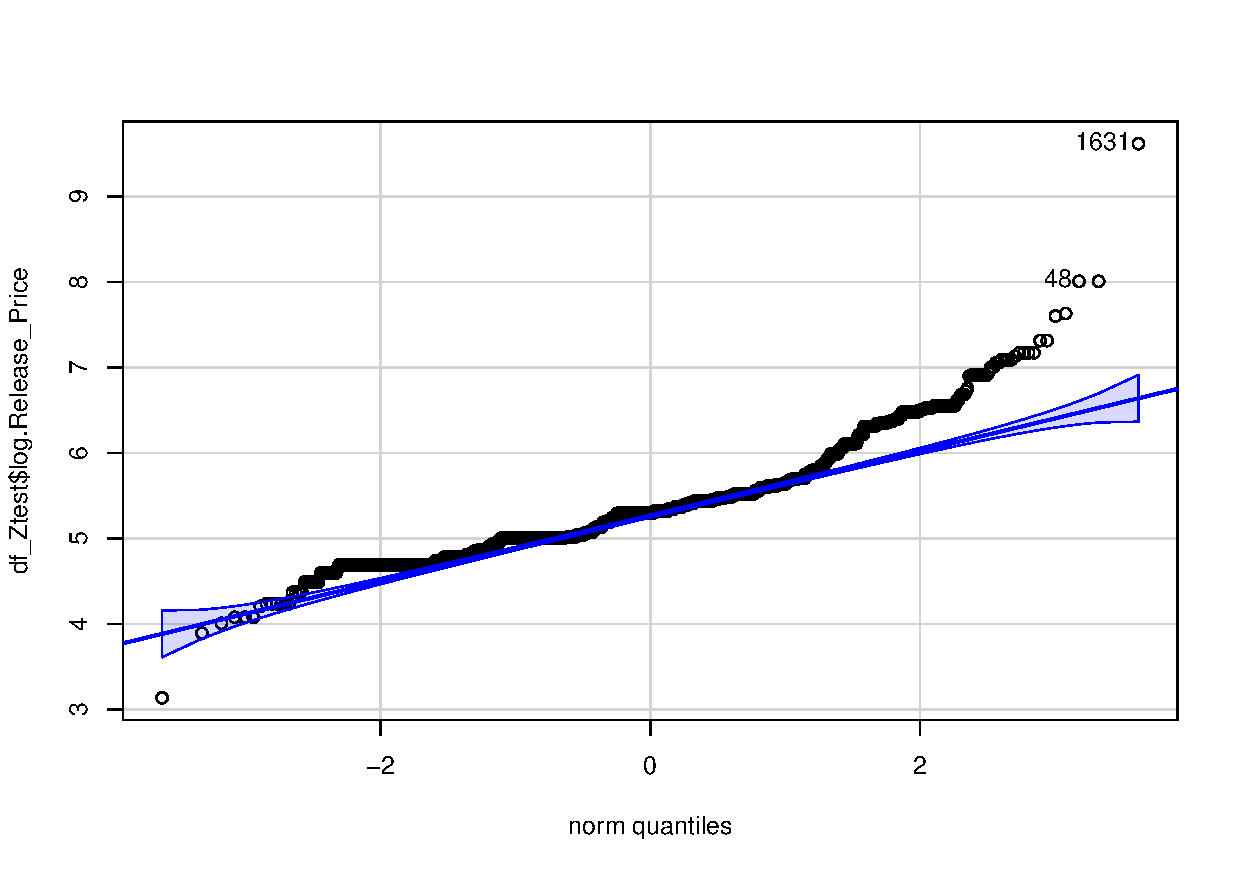
\includegraphics[keepaspectratio, width=1\textwidth, height=1\textheight]{Hypothesis/Z-Test/Ztest-QQPlot.pdf}
\end{figure}
According to the plot above, the data are not normally distributed. Nonetheless the sample size is sufficiently large ($>200$), the normality assumption is not needed at all as the Central Limit Theorem ensures that the distribution of disturbance term will approximate normality. \\\\
\textbf{Condition 3}:\\
We use RStudio to again perform Levene-test on the \verb|df_ztest| dataset to evaluate if the variances of the two populations are equal:
\begin{mdframed}[leftline=false,rightline=false,backgroundcolor=lightblue!10,nobreak=false]
    \begin{minted}[linenos,breaklines,breaksymbolleft=,obeytabs=true,tabsize=2]{R}
leveneTest(log.Release_Price~Manufacturer,df_ztest, center=mean)
    \end{minted}
\end{mdframed}
\begin{lstlisting}
 Levene's Test for Homogeneity of Variance (center = mean)
         Df F value    Pr(>F)    
 group    1  210.25 < 2.2e-16 ***
       3022                      
 ---
 Signif. codes:  0 '***' 0.001 '**' 0.01 '*' 0.05 '.' 0.1 ' ' 1
\end{lstlisting}
From the output above, we can see that the p-value \verb|(< 2.2e-16)| is much smaller compares to the alpha level 0.05. Now we reject the null hypothesis $H_0$ that all populations are equal, which also means there is a difference among the two manufacturers.
\subsubsubsection{Welch’s test}
Because of the condition 3 above is not satisfied for the two-sample Z-test, we will use the Welch’s test instead. There are two hypothesis in the Welch’s test:

\begin{itemize}
    \item Null hypothesis $H_0$: For the test is that the means are equal.
    \item Alternative hypothesis $H_1$: For the test is that means are not equal.
\end{itemize}
Recall the formula of Welch’s test:
\begin{equation*}
    t = \dfrac{\overline{X_1}-\overline{X_2}}{\sqrt{\dfrac{s^2_1}{n_1}+\dfrac{s^2_2}{n_2}}}=\dfrac{\overline{X_1}-\overline{X_2}}{\sqrt{se^2_1+se^2_2}}
\end{equation*}
where:
\begin{itemize}
    \item $\overline{X_i}$ is the $i^{th}$ sample mean.
    \item $s_i$ is the $i^{th}$ standard deviation.
\end{itemize}
Now we perform the Welch’s test in RStudio:
\begin{mdframed}[leftline=false,rightline=false,backgroundcolor=lightblue!10,nobreak=false]
    \begin{minted}[linenos,breaklines,breaksymbolleft=,obeytabs=true,tabsize=2]{R}
oneway.test(log.Release_Price ~ Manufacturer, data=df_ztest)
    \end{minted}
\end{mdframed}
\begin{lstlisting}
 One-way analysis of means (not assuming equal variances)

 data:  log.Release_Price and Manufacturer
 F = 125.23, num df = 1.0, denom df = 2869.3, p-value < 2.2e-16
\end{lstlisting}
\bigskip
\textbf{Conclusion}:
According to the Welch’s test, the p-value shows that we can reject the null hypothesis, and this proves the difference in average release prices between Nvidia and AMD manufacturers.\\

\subsection{Chi-squared test}

A Chi-square test is a hypothesis testing method. Tests involve checking if observed frequencies in one or more categories match expected frequencies. One of them is a test for independence compares two variables in a contingency table to see if they are related.

\subsubsection{Chi-Squared Test of Independence}
\subsubsubsection{Basic concept}
The Chi-Squared Test of Independence can only compare categorical variables. It cannot make comparisons between continuous variables or between categorical and continuous variables. Additionally, the Chi-Square Test of Independence only assesses associations between categorical variables and can not provide any inferences about causation. \cite{bib10, bib13}.\bigskip\\
In this part, we want to find out if there is a relation between the core speed of GPUs and their prices.\bigskip\\ 
To compute Chi-squared test, the data in \verb|df| must meet the follow requirements:
\begin{itemize}
    \item Two categorical variables.
    \item Two or more categories (groups) for each variable.
    \item Independence of observations.
    \begin{itemize}
        \item There is no relationship between the subjects in each group.
        \item The categorical variables are not “paired” in any way.
    \end{itemize}
    \item Relatively large sample size.
    \begin{itemize}
        \item Expected frequencies for each cell are at least 1.
        \item Expected frequencies should be at least 5 for the majority (80\%) of the cells.
    \end{itemize}
\end{itemize}
\subsubsubsection{Building test}
The null hypothesis $(H_0)$ and alternative hypothesis $(H_1)$ of the Chi-Square Test of Independence can be expressed in this way:
\begin{itemize}
    \item $H_0$: Core speed is independent of price, which means knowing the value of core speed does not help to predict the value of the price.
    \item $H_1$: Core speed is associated with price.
\end{itemize}
We will use significant level $\alpha$ = 0.05.\\
The test statistic for the Chi-squared test of Independence is denoted $X^2$, and is computed as:
\begin{equation*}
    X^2= \sum_{i=1}^R \sum_{j=1}^C \dfrac{o_{ij}-e_{ij}}{e_{ij}}
\end{equation*}
where:
\begin{itemize}
    \item $o_{ij}$ is the observed cell count in the $i^{th}$ row and $j^{th}$ column of the table.
    \item $e_{ij}$  is the expected cell count in the $i^{th}$ row and $j^{th}$ column of the table, computed as:
    \begin{equation*}
        e_{ij}=\dfrac{\mathrm{row}_i \mathrm{\:total} \times \mathrm{col}_j \mathrm{\:total}}{\mathrm{grand\:total}}
    \end{equation*}
\end{itemize}
The calculated $X^2$ value is then compared to the critical value from the $X^2$ distribution table with degrees of freedom $df = (R - 1)(C - 1)$ and chosen confidence level. If the calculated $X^2$ value $>$ critical $X^2$ value, then we reject the null hypothesis.\\
Another way to find out answer is through the p-value, if it is less than a pre-determined significance level, which is 0.05 usually, then we reject the null hypothesis.\bigskip\\ 
In our case, we decide to divide \verb|Core_Speed| into 2 levels high $(>7)$ and low $(<7)$ as 7 is the mean of \verb|log.Core_Speed| and the price into 3 ranges:
\begin{itemize}
    \item Cheap (3-5).
    \item Medium (5-7).
    \item Expensive ($>$7).
\end{itemize}
\begin{mdframed}[leftline=false,rightline=false,backgroundcolor=lightblue!10,nobreak=false]
    \begin{minted}[linenos,breaklines,breaksymbolleft=,obeytabs=true,tabsize=2]{R}
HighCoreSpeed <- filter(df, log.Core_Speed > 7)
LowCoreSpeed <- filter(df, log.Core_Speed < 7)
    \end{minted}
\end{mdframed}
After filter, we have this table:
\begin{table}[!htb]
\centering
\begin{tabular}{|c|ccc|c}
\cline{1-4}
\multirow{2}{*}{\texttt{log.Core\_Speed}} & \multicolumn{3}{c|}{\texttt{log.Release\_Price}}                                                                       &  \\ \cline{2-4}
                                & \multicolumn{1}{l|}{Cheap (3-5)} & \multicolumn{1}{l|}{Medium (5-7)} & \multicolumn{1}{l|}{Expensive (7-10)} &  \\ \cline{1-4}
High (\textgreater{}7)           & \multicolumn{1}{c|}{80}         & \multicolumn{1}{c|}{530}         & 8                                    &  \\ \cline{1-4}
Low (\textless{}7)               & \multicolumn{1}{c|}{372}        & \multicolumn{1}{c|}{2362}        & 12                                   &  \\ \cline{1-4}
\end{tabular}
\end{table}\\
The next step is to compute Chi-squared test in R. Chi-squared statistic can be easily computed as follow:
\begin{mdframed}[leftline=false,rightline=false,backgroundcolor=lightblue!10,nobreak=false]
    \begin{minted}[linenos,breaklines,breaksymbolleft=,obeytabs=true,tabsize=2]{R}
HighCoreSpeed  = c(80,530,8)
LowCoreSpeed  = c(373,2362,12)
chisq.test(data.frame(HighCoreSpeed ,LowCoreSpeed))
    \end{minted}
\end{mdframed}

\begin{lstlisting}
     Pearson's Chi-squared test

 data:  data.frame(HighCoreSpeed, LowCoreSpeed)
 X-squared = 6.3971, df = 2, p-value = 0.04082
\end{lstlisting}
\textbf{Conclusion}: We can say that since the p-value is smaller than our chosen significance level ($\alpha$ = 0.05), we can reject the null hypothesis. Rather, we conclude that the two variables are in fact dependent.
%%%%%%%%%%%%%%%%%%%%%%%%%%%%%%%%%%%%%%%%%%%%%%%%%%%%%%%%%%%%%%%%%%


\section{Fitting linear regression model}
Since the price of GPU is affected by many factors, we choose multiple regression model instead of simple regression model (single factor).
\subsection{Fast introduction to multiple linear regression}
A well-fitting regression model results in predicted values close to the observed data values. The mean model, which uses the mean for every predicted value, generally would be used if there were no informative predictor variables. Therefore, the fit of a proposed regression model will be better than the fit of the mean model.\\\\
By fitting a line to the observed data, we can describe how strong the relationship is between one or more independent variables and one dependent variable (how a dependent variable changes as the independent variable(s) change), or find the value of the dependent variable at a certain value of the independent variable(s). Given the data set we acquired, a multiple linear regression model is reasonable with the goal of observing how the dependent variable Release\_Price would change under the influence of other variables.\\\\
A multiple linear regression model generally has the formula:\\
\begin{equation*}
    y = \beta_{0}+ \beta_{1} X_{1} + ... + \beta_{n}  X_{n} + \epsilon
\end{equation*}
where:
\begin{itemize}
    \item $y$ is the predicted value of the dependent variable.
    \item $\beta_{0}$ is the $y$-intercept (value of $y$ when all other parameters are set to 0).
    \item $\beta_{1} X_{1}$ is the regression coefficient of the first independent variable.
    \item $\beta_{n} X_{n}$ is the regression coefficient of the last independent variable.
    \item $e$ is the model error a.k.a. how much variation there is in our estimate of $y$.
\end{itemize}
To find the best-fit line for each independent variable, multiple linear regression calculates three things:
\begin{itemize}
    \item The regression coefficients that lead to the smallest overall model error.
    \item The t-statistic of the overall model.
    \item The associated p-value (how likely it is that the t-statistic would have occurred by chance if the null hypothesis of no relationship between the independent and dependent variables was true).
    \item It then calculates the t-statistic and p-value for each regression coefficient in the model.
\end{itemize}

\subsection{Constructing multiple linear regression model}
We choose multiple linear regression model because the price of GPU depends on many factors.
\subsubsection{Defining input and output}
\begin{itemize}
    \item Input: 
    \begin{itemize}
        \item \verb|Boost_Clock|
        \item \verb|Core_Speed|
        \item \verb|Max_Power|
        \item \verb|Memory|
        \item \verb|Memory_Bus|
        \item \verb|Memory_Speed|
        \item \verb|Shader|
        \item \verb|TMUs|
        \item \verb|Release_Price|
    \end{itemize}
    \item Output:
    \begin{itemize}
        \item The multiple linear regression model with \verb|Release_Price| is a dependent variable.
    \end{itemize}
\end{itemize}

\subsubsection{Linear regression model \texttt{lmPrice}}
In this section we will implement the model and we will explain it in detail in the next section. By using the function \verb|lm()| included in R:
\begin{mdframed}[leftline=false,rightline=false,backgroundcolor=lightblue!10,nobreak=false]
    \begin{minted}[linenos,breaklines,breaksymbolleft=,obeytabs=true,tabsize=2]{R}
lmPrice = lm(log.Release_Price ~ log.Boost_Clock + log.Core_Speed + log.Max_Power + log.Memory + log.Memory_Bus + log.Memory_Speed + log.Shader + log.TMUs, df)
summary(lmPrice)
    \end{minted}
\end{mdframed}
\begin{lstlisting}
 Call:
 lm(formula = log.Release_Price ~ log.Boost_Clock + log.Core_Speed + 
     log.Max_Power + log.Memory + log.Memory_Bus + log.Memory_Speed + 
     log.Shader + log.TMUs, data = df)

 Residuals:
     Min      1Q  Median      3Q     Max 
 -1.5408 -0.1914 -0.0409  0.1517  3.4111

 Coefficients:
                   Estimate Std. Error t value Pr(>|t|)    
 (Intercept)       2.159859   0.279644   7.724 1.48e-14 ***
 log.Boost_Clock   0.596747   0.041774  14.285  < 2e-16 ***
 log.Core_Speed   -0.307610   0.020964 -14.673  < 2e-16 ***
 log.Max_Power     0.154701   0.011974  12.920  < 2e-16 ***
 log.Memory        0.149222   0.009817  15.200  < 2e-16 ***
 log.Memory_Bus    0.187296   0.015686  11.940  < 2e-16 ***
 log.Memory_Speed -0.159942   0.022510  -7.106 1.46e-12 ***
 log.Shader       -0.551948   0.041147 -13.414  < 2e-16 ***
 log.TMUs          0.076648   0.011044   6.940 4.68e-12 ***
 ---
 Signif. codes:  0 '***' 0.001 '**' 0.01 '*' 0.05 '.' 0.1 ' ' 1

 Residual standard error: 0.3122 on 3356 degrees of freedom
 Multiple R-squared:  0.5231,	Adjusted R-squared:  0.522 
 F-statistic: 460.1 on 8 and 3356 DF,  p-value: < 2.2e-16

\end{lstlisting}

\subsubsection{Explanation}

\subsubsubsection{The \texttt{lm()} function}
R linear regression uses the \verb|lm()| function to create a regression model given some formula, in the form of
\begin{equation*}
    Y \sim X_1 + X_2 + ...
\end{equation*}
In our linear regression model:
\begin{itemize}
    \item The independent $X_i$ (predictor or random) variables:
    \begin{itemize}
        \item \verb|Boost_Clock|
        \item \verb|Core_Speed|
        \item \verb|Max_Power|
        \item \verb|Memory|
        \item \verb|Memory_Bus|
        \item \verb|Memory_Speed|
        \item \verb|Shader|
        \item \verb|TMUs|
    \end{itemize}
    \item The dependent $Y$ variable (the one we are trying to predict):
    \begin{itemize}
        \item \verb|Release_Price|
    \end{itemize}
    \item Data source: The data frame \verb|df|.
\end{itemize}

\subsubsubsection{The \texttt{summary()} function} 
The \texttt{summary()} is an inbuilt generic function in R used to produce result summaries of various model fitting functions. It returns:
\begin{enumerate}
    \item \verb|Residuals|: The section summarizes the residuals, the error between the prediction of the model and the actual results. 
    \begin{itemize}
        \item The \verb|min/max| and quantiles \verb|Q1/Median/Q3| for the distribution of the residuals.
    \end{itemize}
    
    \item \verb|Coefficients|
    \begin{itemize}
        \item The values of the \verb|intercept| (\textcolor{blue}{\texttt{a}} value) and the slope (\textcolor{blue}{\texttt{b}} value) for the other attributions are in the first column.
        \item \verb|Estimate|:  The weight given to the variable. For every one unit of above attributes change, the model predicts a change of \verb|Release_Price| as this equation:
        \begin{align*}
            \texttt{Release\_Price =} &\texttt{ + 0.596747 $\times$ Boost\_Clock - 0.307610 $\times$ Core\_Speed}\\ 
            &\texttt{ + 0.154701 $\times$ Max\_Power + 0.149222 $\times$ Memory}\\
            &\texttt{ + 0.187296 $\times$ Memory\_Bus - 0.159942 $\times$ Memory\_Speed}\\
            &\texttt{ - 0.551948 $\times$ Shader + 0.076648 $\times$ TMUs + 2.159859}
        \end{align*}
        
        \item \verb|Std. Error|: The standard error.
        \item \verb|t value|:  A measure of how many standard deviations our coefficient estimate is far away from 0. Calculated by the formula:
        \begin{equation*}
            t_{value} = \dfrac{Estimate}{Std. Error}
        \end{equation*}
         A larger t-value indicates that it is less likely that the coefficient is not equal to zero purely by chance. Therefore, the higher the t-value, the better.
         \item \texttt{Pr(>|t|)}: The probability of observing any value equal or larger than t-value.
    \end{itemize}
    
    \item \verb|Signif. codes|: A legend for the number of stars next to the p-value. For example, the \verb|Max_Power| attribute has a p-value of \verb|<2e-16|. Since this value is in the range \verb|[0, 0.001]|, it has a significance code of \verb|***|.
    
    \item \verb|Residual standard error|: A measure of the quality of a linear regression fit (the standard deviation of the residuals). Calculated by the formula:
    \begin{align*}
        SSE &= \sum_{i=1}^n(y_i-\hat{y}_i)^2\\
        \delta &= \sqrt{\frac{SSE}{df}}
    \end{align*}
    where:
    \begin{itemize}
        \item $\delta$ = Residual Standard Error.
        \item $df = n - (k + 1)$ = Degrees of Freedom:
        \begin{itemize}
            \item $n$ = Number of observations.
            \item $k+1$ = Number of coefficients including intercepts.
        \end{itemize}
    \end{itemize}
    
    \item \verb|Multiple R-squared|: A measure of how well the model is fitting the actual data. It indicates the proportion of the variance in the model that is explained by the model. Perfect is 1, none is 0.
    \begin{align*}
        SST &= \sum_{i=1}^n(y_i-\bar{y})^2\\
	    SSE &= \sum_{i=1}^n(y_i-\hat{y}_i)^2\\
	    SSR &= \sum_{i=1}^n(\hat{y}_i-\bar{y})^2\\
	    R^2 &= 1 - \dfrac{SSE}{SST} = \dfrac{SSR}{SST}
    \end{align*}
    
    \item \verb|Adjusted R-squared|: The preferred measure as it adjusts for the number of variables considered.
    \begin{align*}
        &MSE = \frac{SSE}{n-k}\\
	    &MST = \frac{SST}{n-1}\\
	    &R^2_{adj} = 1 - \dfrac{MSE}{MST} = 1 - \dfrac{(1-R^2)(n-1)}{n-k}
    \end{align*}
    
    \item \verb|F-statistic|: A indicator of whether there is a relationship between our predictor and the response variables (a test to see if a model with fewer parameters will be better).
    \begin{itemize}
        \item \verb|p-value|: A low value indicates that our model is probably better than a model with fewer parameters (i.e. there is little chance that the results are random).
        \begin{equation*}
            MSR = \dfrac{\sum_{i=1}^n(\hat{y}_i-\bar{y})^2}{k-1} = \dfrac{SST-SSE}{k-1}
        \end{equation*}
        
        \item “Is the regression model containing at least one predictor useful in predicting price?”.\\
        To answer the research question, we test the hypothesis testing:
        \begin{align*}
            &H_0:\beta_1=\beta_2=...=\beta_n\\
            &H_1:\exists \beta_i \ne 0
        \end{align*}
        \begin{itemize}
            \item The full model\\
            This is the largest possible model - that is, the model containing all of the possible predictors. In this case, the full model is:
            \begin{equation*}
                y_i = \alpha + (\beta_1 x_1 + \beta_2 x_2 +...+\beta_n x_n) + \varepsilon_i
            \end{equation*}
            There are $k$ predictors in the full model and the number of error degrees of freedom associated with the full model is: $df_R=n-(k+1)$.
            \item The reduced model\\
            This is the model that the null hypothesis describes:
            \begin{equation*}
                y_i = \alpha + \varepsilon_i
            \end{equation*}
            The reduced model basically suggests that none of the variation in the response y is explained by any of the predictors. Therefore, the number of error degrees of freedom associated with the reduced model is $df_R=n-1$.\\
            We use the general linear \verb|F-statistic| to decide whether or not:
            \begin{itemize}
                \item To reject the null hypothesis $H_0$: The reduced model.
                \item In favor of the alternative hypothesis $H_1$: The full model.
            \end{itemize}
            In general, we reject $H_0$ if \verb|F-statistic| is large - or equivalently if its associated \verb|p-value| is small. 
        \end{itemize}
    \end{itemize}
\end{enumerate}
\subsection{Considering eliminating any the independent variables due to the \texttt{Pr(>[t])}}
From the result of \verb|summary()| function, if we choose the confidence (significant) level at 0.05, we can keep all the variables:
\begin{itemize}
    \item \verb|Boost_Clock| (2$\times 10^{-16} \ll$ 0.05)
    \item \verb|Core_Speed| (2$\times 10^{-16} \ll$ 0.05)
    \item \verb|Max_Power| (2$\times 10^{-16} \ll$ 0.05)
    \item \verb|Memory| (2$\times 10^{-16} \ll$ 0.05)
    \item \verb|Memory_Bus| (2$\times 10^{-16} \ll$ 0.05)
    \item \verb|Memory_Speed| (1.46$\times 10^{-12} \ll$ 0.05)
    \item \verb|Shader| (2$\times 10^{-16} \ll$ 0.05)
    \item \verb|TMUs| (4.68$\times 10^{-12} \ll$ 0.05)
\end{itemize}
It is clear that the probability of simultaneously rejecting $H_0$ of the above 8 variables is very high, so we have enough evidence to reject the null hypothesis $H_0$ that those coefficients are equal to 0.


\subsection{Testing the linear regression model}
\begin{align*}
    \texttt{lmPrice}: &\text{ Linear regression model includes all the variables}.\\
    \texttt{lmPriceNoMem}: &\text{ Linear regression model without variable \texttt{Memory}}.
\end{align*}
\subsubsection{Linear regression model \texttt{lmPriceNoMem}}
We construct the linear regression model \verb|lmPriceNoMem|:
\begin{mdframed}[leftline=false,rightline=false,backgroundcolor=lightblue!10,nobreak=false]
    \begin{minted}[linenos,breaklines,breaksymbolleft=,obeytabs=true,tabsize=2]{R}
lmPriceNoMem = lm(log.Release_Price ~ log.Boost_Clock + log.Core_Speed + log.Max_Power + log.Memory_Bus + log.Memory_Speed + log.Shader + log.TMUs, df)
summary(lmPriceNoMem)
    \end{minted}
\end{mdframed}
\begin{lstlisting}
 Call:
 lm(formula = log.Release_Price ~ log.Boost_Clock + log.Core_Speed + 
     log.Max_Power + log.Memory_Bus + log.Memory_Speed + log.Shader + 
     log.TMUs, data = df)

 Residuals:
     Min      1Q  Median      3Q     Max 
 -1.6128 -0.1909 -0.0541  0.1503  3.6845  

 Coefficients:
                  Estimate Std. Error t value Pr(>|t|)    
 (Intercept)       0.92795    0.27666   3.354 0.000805 ***
 log.Boost_Clock   0.73613    0.04213  17.473  < 2e-16 ***
 log.Core_Speed   -0.30055    0.02166 -13.872  < 2e-16 ***
 log.Max_Power     0.16255    0.01237  13.145  < 2e-16 ***
 log.Memory_Bus    0.21411    0.01611  13.289  < 2e-16 ***
 log.Memory_Speed -0.06736    0.02240  -3.007 0.002655 ** 
 log.Shader       -0.30204    0.03899  -7.746 1.24e-14 ***
 log.TMUs          0.10841    0.01121   9.671  < 2e-16 ***
 ---
 Signif. codes:  0 '***' 0.001 '**' 0.01 '*' 0.05 '.' 0.1 ' ' 1

 Residual standard error: 0.3228 on 3357 degrees of freedom
 Multiple R-squared:  0.4903,	Adjusted R-squared:  0.4892 
 F-statistic: 461.3 on 7 and 3357 DF,  p-value: < 2.2e-16
\end{lstlisting}
After removing \verb|Memory| attribute, the \verb|R_squared| decrease, the adequacy of this model is still recognized and the \verb|p-value| (\verb|2.2e-16|) is much less than ($\ll$) significance value (\verb|0.05|) which implies that the hypothesis that the intercept is zero is rejected. However, the model \verb|lmPrice| still better than, see more in the next section.
\subsubsection{Comparison}
We use \verb|anova()| function to test the linear regression model to related \verb|Release_Price| to \verb|Memory|.

\begin{mdframed}[leftline=false,rightline=false,backgroundcolor=lightblue!10,nobreak=false]
    \begin{minted}[linenos,breaklines,breaksymbolleft=,obeytabs=true,tabsize=2]{R}
lmPrice_Mem = lm(log.Release_Price ~ log.Memory, df[, c('log.Release_Price', 'log.Memory')])
anova(lmPrice_Mem)
    \end{minted}
\end{mdframed}
\begin{lstlisting}
 Analysis of Variance Table

 Response: log.Release_Price
             Df Sum Sq Mean Sq F value    Pr(>F)    
 log.Memory    1 140.28 140.284  864.38 < 2.2e-16 ***
 Residuals  3363 545.80   0.162                    
 ---
 Signif. codes:  0 '***' 0.001 '**' 0.01 '*' 0.05 '.' 0.1 ' ' 1
\end{lstlisting}
Hypothesis:
\begin{align*}
    H_0: &\text{ \texttt{Release\_Price} does not depend on the variation of \texttt{Memory}}.\\
    H_1: &\text{ \texttt{Release\_Price} depends on the variation of \texttt{Memory}}.
\end{align*}
Based on the result of the \verb|anova()| testing, the \verb|p-value| (\verb|2.2e-16|) is much less than ($\ll$) significance value (\verb|0.05|) which is a strong evidence of removing the null hypothesis $H_0$, admitting the dependence of \verb|Release_Price| on \verb|Memory|.\\
$\Rightarrow$ The model \verb|lmPrice| is more accurate than the model \verb|lmPriceNoMem|.

\subsection{Model accuracy assessment}
The overall quality of the model can be assessed by examining the R-squared ($R^2$), the Residual Standard Error ($RSE$) and F-Statistic.\\
We recall the summary of the model \verb|lmPrice|:
\begin{lstlisting}
 Residual standard error: 0.312 on 3356 degrees of freedom
 Multiple R-squared:  0.523,	Adjusted R-squared:  0.522 
 F-statistic:  460 on 8 and 3356 DF,  p-value: <2e-16
\end{lstlisting}
\subsubsection{R-square}
In multiple linear regression, the $R^2$ represents the correlation coefficient between the observed values of the outcome variable ($y$) and the fitted (i.e. predicted) values of $y$. For this reason, the value of $R$ will always be positive and will range from zero to one.\\\\
$R^2$ represents the proportion of variance, in the outcome variable $y$, that may be predicted by knowing the value of the $x$ variables. An $R^2$ value close to 1 indicates that the model explains a large portion of the variance in the outcome variable.\\\\
A problem with the $R^2$, is that, it will always increase when more variables are added to the model, even if those variables are only weakly associated with the response. A solution is to adjust the $R^2$ by taking into account the number of predictor variables.\\\\
The adjustment in the \verb|Adjusted R Square| value in the summary output is a correction for the number of $x$ variables included in the prediction model.\\\\
In our multiple regression model, with 8 variables, the \verb|Adjusted R-squared = 0.522|, meaning that “52.2\% of the variance in the measure of price can be predicted by 8 variables”.
\subsubsection{Residual Standard Error}
The $RSE$ (or sigma $\sigma$) estimate gives a measure of error of prediction. The lower the $RSE$, the more accurate the model (on the data in hand).\\
The error rate can be estimated by dividing the $RSE$ by the mean outcome variable:
\begin{mdframed}[leftline=false,rightline=false,backgroundcolor=lightblue!10,nobreak=false]
    \begin{minted}[linenos,breaklines,breaksymbolleft=,obeytabs=true,tabsize=2]{R}
sigma(lmPrice)/mean(df$log.Release_Price)
    \end{minted}
\end{mdframed}

\begin{lstlisting}
 0.0585
\end{lstlisting}
In our multiple regression model, the $RSE$ is \verb|0.312|  corresponding to 5.85\% error rate.

\subsubsection{F-Statistic}
Recall that, the F-statistic gives the overall significance of the model. It assess whether at least one predictor variable has a non-zero coefficient.\\\\
In a simple linear regression, this test is not really interesting since it just duplicates the information given by the t-test, available in the coefficient table.\\\\
The F-statistic becomes more important once we start using multiple predictors as in multiple linear regression.\\\\
A large F-statistic will corresponds to a statistically significant p-value (p $<$ 0.05). In our example, the F-statistic equal \verb|460| producing a \verb|p-value| of \verb|<2e-16|, which is highly significant.

\subsection{Multicollinearity checking}
One of the assumptions of the Classical Linear Regression Model \cite{bib7} is that there is no exact collinearity between the explanatory variables. If the explanatory variables are perfectly correlated, the following problems are faced:
\begin{itemize}
    \item Parameters of the model become indeterminate.
    \item Standard errors of the estimates become infinitely large.
\end{itemize}
However, the case of perfect collinearity is very rare in practical cases. Imperfect or less than perfect multicollinearity is the more common problem and it arises when in multiple regression modelling two or more of the explanatory variables are approximately linearly related.\\\\
In multiple regression, two or more predictor variables might be correlated with each other. This situation is referred as collinearity. And so, as a result:
\begin{itemize}
    \item Estimates for regression coefficients of the independent variables can be unreliable.
    \item Tests of significance for regression coefficients can be misleading.
\end{itemize}
In the presence of multicollinearity, the solution of the regression model becomes unstable. For a given predictor (p), multicollinearity can assessed by computing a score called the variance inflation factor (or VIF), which measures how much the variance of a regression coefficient is inflated due to multicollinearity in the model \cite{bib8}. Here is the formula for calculating VIF:
\begin{equation*}
    VIF_i=\dfrac{1}{1-R_i^2}
\end{equation*}
where:
\begin{itemize}
    \item $R_i^2$ is the coefficient of determination of the linear regression equation, 
    \item $i$  is index number of variables in the linear regression model.
\end{itemize}
The smallest possible value of VIF is one (absence of multicollinearity). As a rule of thumb, a VIF value that exceeds 5 or 10 indicates a problematic amount of collinearity.\\\\
When faced to multicollinearity, the concerned variables should be removed, since the presence of multicollinearity implies that the information that this variable provides about the response is redundant in the presence of the other variables.\\\\
Now we will test our model using \verb|vif()| function:
\begin{mdframed}[leftline=false,rightline=false,backgroundcolor=lightblue!10,nobreak=false]
    \begin{minted}[linenos,breaklines,breaksymbolleft=,obeytabs=true,tabsize=2]{R}
vif(lmPrice)
    \end{minted}
\end{mdframed}
\begin{lstlisting}
 log.Boost_Clock   log.Core_Speed    log.Max_Power 
        1.577571         2.364690         4.123739 
      log.Memory   log.Memory_Bus log.Memory_Speed 
        3.874111         2.807052         4.012138 
      log.Shader         log.TMUs 
        2.520362         5.664969 
\end{lstlisting}
In our model, the VIF score for the predictor variable \verb|TMUs| is a bit high (VIF = \verb|5.664969|). This might be problematic. However, it seems that we can assume that the model is free from multicollinearity.

\subsection{Confidence interval}
We want to computes 95\% confidence intervals for each variable in our model. Using \verb|confint()| function:
\begin{center}
    \verb|confint(object, parm, level = 0.95, …)|
\end{center}
\begin{itemize} 
    \item \verb|object|: A fitted model object, here we pass our \verb|lmPrice| model.
    \item \verb|parm|: A specification of which parameters are to be given confidence intervals, either a vector of numbers or a vector of names. If missing, all parameters are considered. We skip this part.
    \item \verb|level|: The confidence level required, default is set to 0.95.
    \item \verb|...|: Additional argument(s) for methods, we skip this part.
\end{itemize}
This function returns a matrix (or vector) with columns giving lower and upper confidence limits for each parameter. These will be labelled as $\dfrac{\mathrm{1 - level}}{2}$ and $1- \dfrac{\mathrm{1 - level}}{2}$ in \% (by default 2.5\% and 97.5\%).
\begin{mdframed}[leftline=false,rightline=false,backgroundcolor=lightblue!10,nobreak=false]
    \begin{minted}[linenos,breaklines,breaksymbolleft=,obeytabs=true,tabsize=2]{R}
confint(lmPrice)
    \end{minted}
\end{mdframed}
\begin{lstlisting}
                   2.5 %  97.5 %
 (Intercept)       1.612  2.7081
 log.Boost_Clock   0.515  0.6787
 log.Core_Speed   -0.349 -0.2665
 log.Max_Power     0.131  0.1782
 log.Memory        0.130  0.1685
 log.Memory_Bus    0.157  0.2181
 log.Memory_Speed -0.204 -0.1158
 log.Shader       -0.633 -0.4713
 log.TMUs          0.055  0.0983
\end{lstlisting}

\subsection{Graphs}
\begin{mdframed}[leftline=false,rightline=false,backgroundcolor=lightblue!10,nobreak=false]
    \begin{minted}[linenos,breaklines,breaksymbolleft=,obeytabs=true,tabsize=2]{R}
plot(lmPrice$fitted.values, lmPrice$residuals, col = "black", xlab = "Fitted values", ylab = "Residuals")
    \end{minted}
\end{mdframed}
\begin{figure}[H]
    \centering
    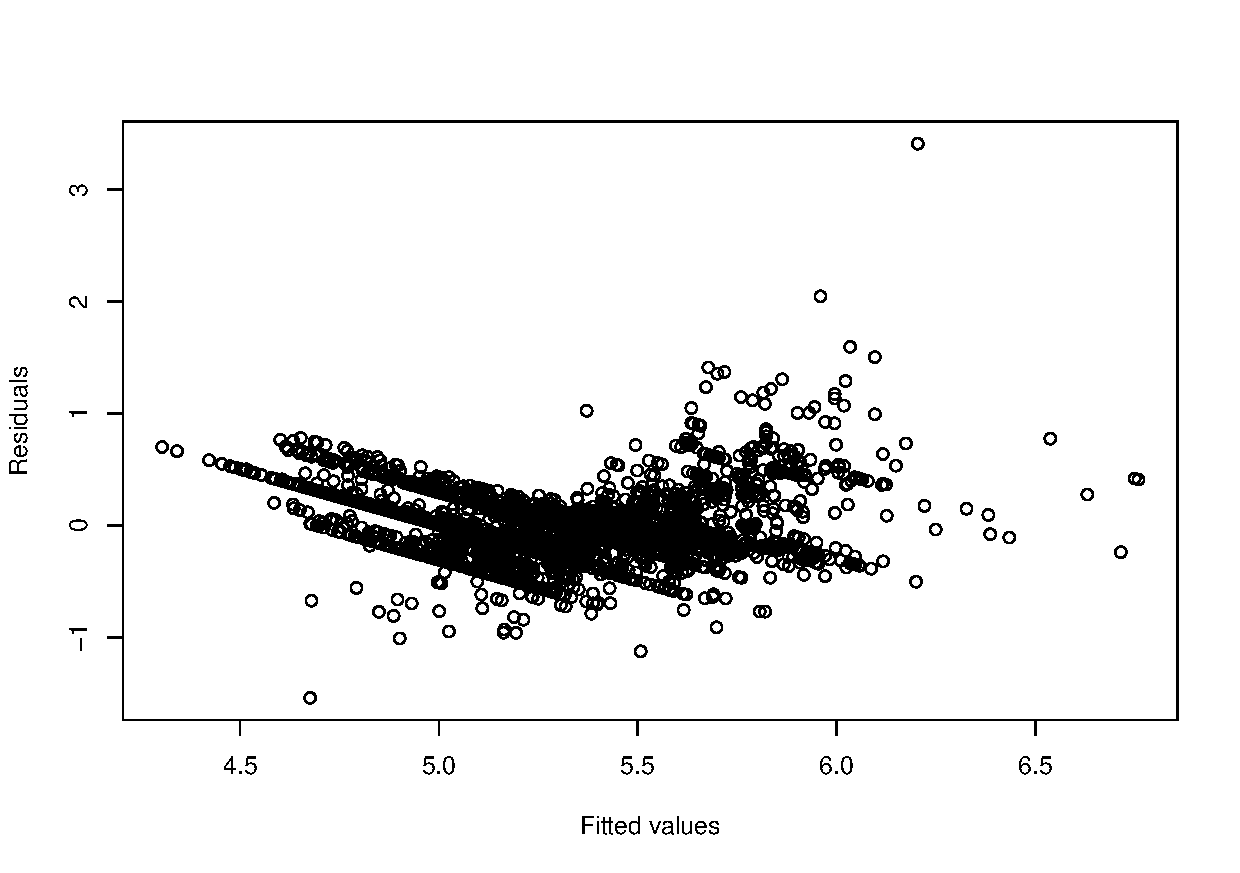
\includegraphics[keepaspectratio, width=1\textwidth, height=1\textheight]{LRM/Rplot.pdf}
\end{figure}
The natural logarithm of the GPU prices fluctuates mostly around $10^{4.5}$ to $10^{6.5}$ and that of the residuals is mostly around -1 to 1 which mean the predicted price and the actual price difference by between $e^{-1}$ and $e^{1}$.
\subsubsection{Homoscedasticity checking}
Homoscedasticity, or homogeneity of variances, is an assumption of equal or similar variances in different groups being compared. The assumption of homoscedasticity (meaning “same variance”) is central to linear regression models.  Homoscedasticity describes a situation in which the error term (that is, the “noise” or random disturbance in the relationship between the independent variables and the dependent variable) is the same across all values of the independent variables.  Heteroscedasticity (the violation of homoscedasticity) is present when the size of the error term differs across values of an independent variable.  The impact of violating the assumption of homoscedasticity is a matter of degree, increasing as heteroscedasticity increases \cite{bib14}.\\\\
We try to plot the equation of our model to make sure that our model fit the homoscedasticity assumption of the linear model.
\begin{mdframed}[leftline=false,rightline=false,backgroundcolor=lightblue!10,nobreak=false]
    \begin{minted}[linenos,breaklines,breaksymbolleft=,obeytabs=true,tabsize=2]{R}
par(mfrow=c(2,2))
plot(lmPrice, col = "black")
par(mfrow=c(1,1))
    \end{minted}
\end{mdframed}
\begin{figure}[H]
    \centering
    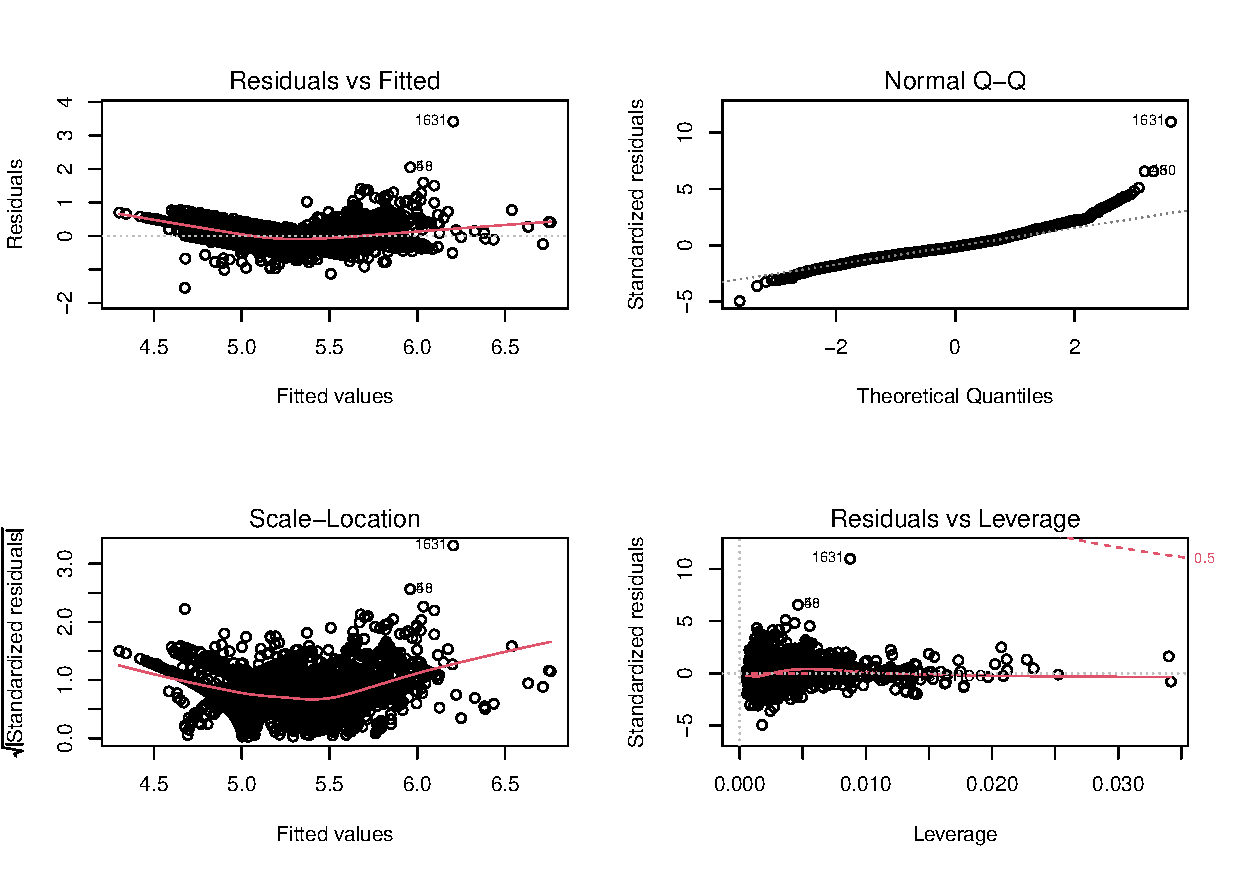
\includegraphics[keepaspectratio, width=1\textwidth, height=1\textheight]{LRM/Rplot2.pdf}
\end{figure}
Note that the \verb|par(mfrow())| command will divide the Plots window into the number of rows and columns specified in the brackets. So \verb|par(mfrow=c(2,2))| divides it up into two rows and two columns. To go back to plotting one graph in the entire window, set the parameters again and replace the \verb|(2,2)| with \verb|(1,1)|.\\
Graph meaning:
\begin{itemize}
    \item \verb|Residuals vs Fitted|: When conducting a residual analysis, this plot is the most frequently created plot. It is a scatter plot of residuals on the $y$-axis and fitted values (estimated responses) on the $x$-axis. The plot is used to detect non-linearity, unequal error variances, and outliers.
    \item \verb|Normal Q-Q|: This is a graphical technique for determining if two datasets come from populations with a common distribution.
    \item \verb|Scale-Location|: This plot shows whether residuals are spread equally along the ranges of input variables (predictor).
    \item \verb|Residuals vs Leverage|: This is a type of diagnostic plot that allows us to identify influential observations in a regression mode. Leverage is a measure of how far away the independent variable values of an observation are from those of the other observations
\end{itemize}
Based on the residual plots:
\begin{itemize}
    \item Residuals are the unexplained variance. They are not exactly the same as model error, but they are calculated from it, so seeing a bias in the residuals would also indicate a bias in the error.
    \item The most important thing to look for is that the red lines representing the mean of the residuals are all basically horizontal and centered around zero. This means there are no outliers or biases in the data that would make a linear regression invalid.
    \item In the \verb|Normal Q-Q| plot in the top right, we can see that the real residuals from our model form an almost perfectly one-to-one line with the theoretical residuals from a perfect model.
    \item We can check the residuals by plotting their histograms and distributions.
\begin{mdframed}[leftline=false,rightline=false,backgroundcolor=lightblue!10,nobreak=false]
    \begin{minted}[linenos,breaklines,breaksymbolleft=,obeytabs=true,tabsize=2]{R}
par(mfrow=c(1, 2))
ggplot(df, aes(x = lmPrice$residuals, y=..density..)) + theme_classic() +  geom_density() +
  geom_histogram(bins = 100, fill = 'steelblue', color = 'black') + 
  labs(title = 'Histogram of Residuals', x = 'Residuals', y = 'Frequency') +
  theme(legend.position='bottom', plot.title = element_text(hjust = 0.5)) 
    \end{minted}
\end{mdframed}
\end{itemize}
\begin{figure}[H]
    \centering
    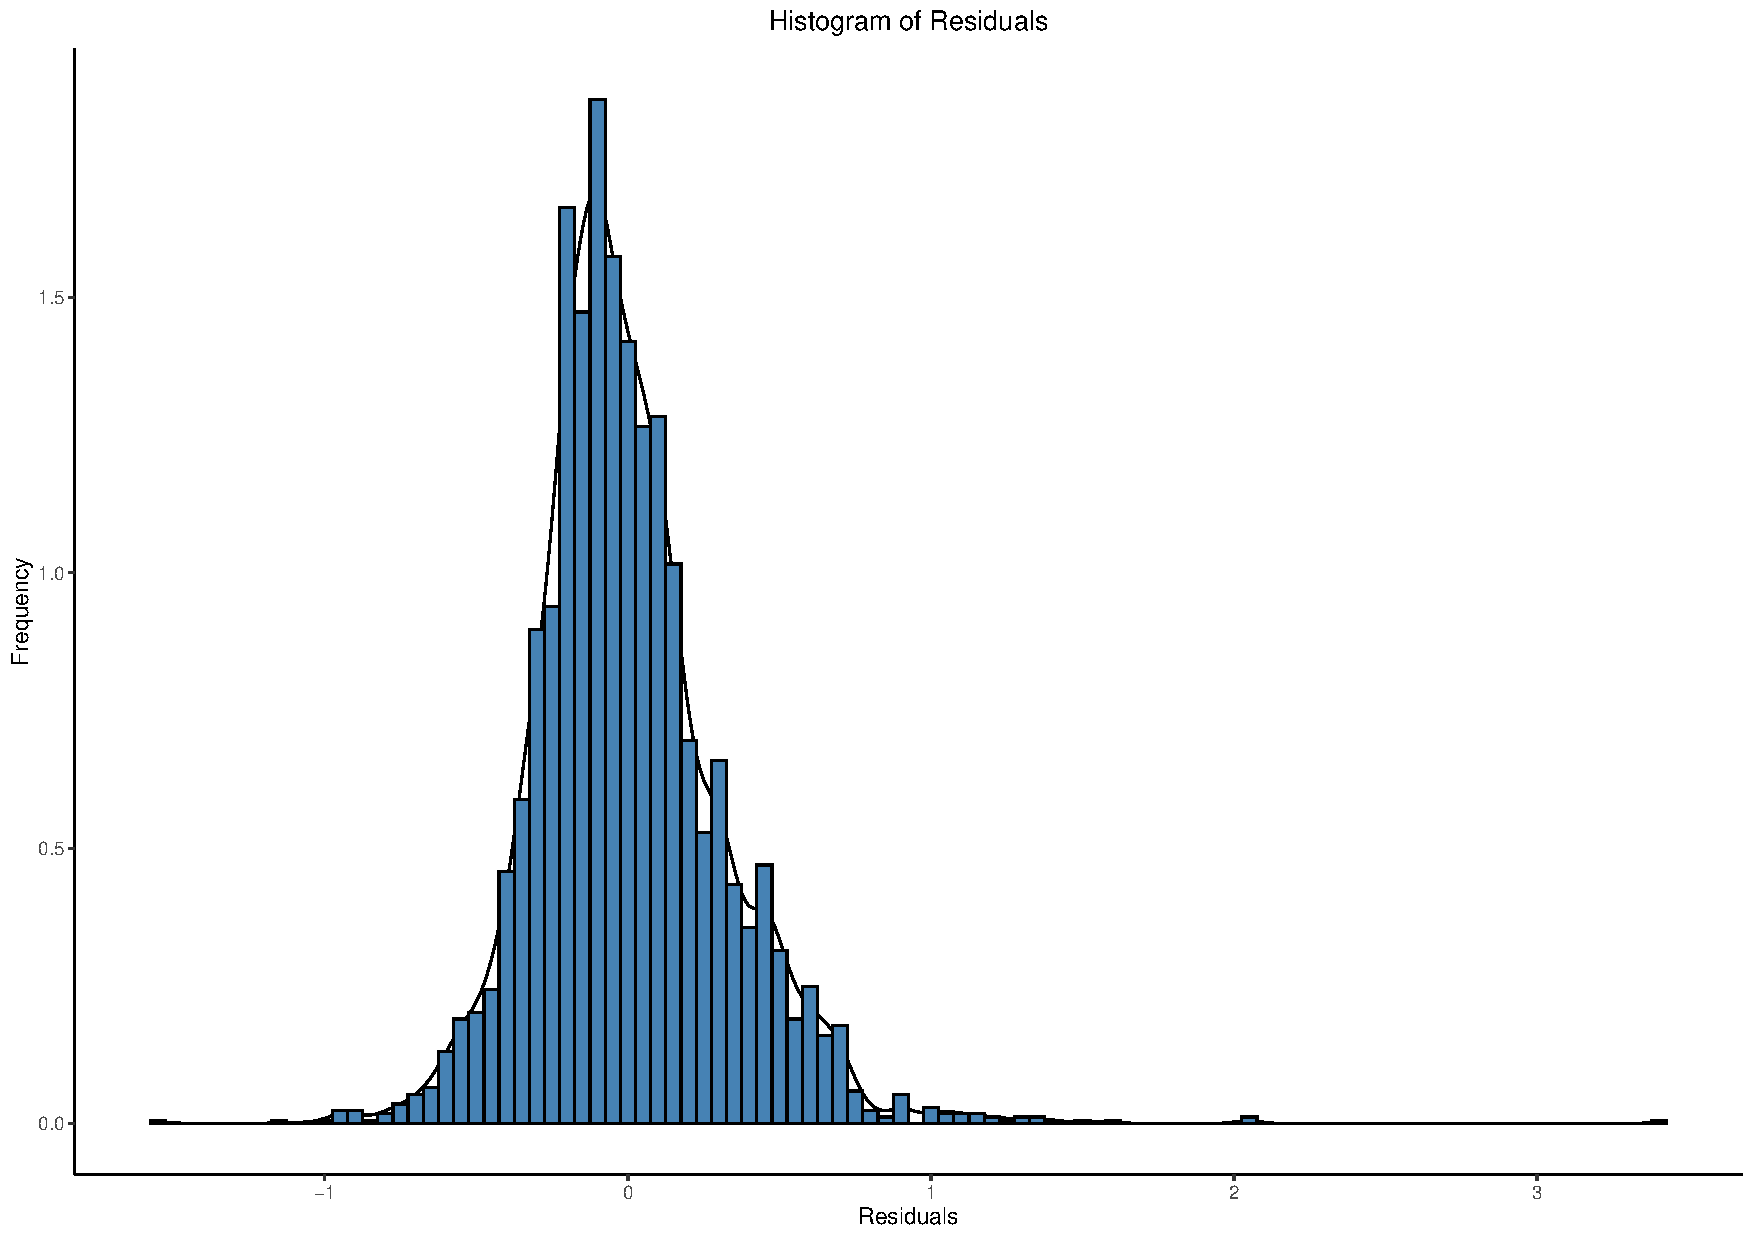
\includegraphics[keepaspectratio, width=1\textwidth, height=1\textheight]{LRM/Rplot10.pdf}
\end{figure}


\begin{itemize}
    \item From the above figure, we can see a “fair” normal distribution.
    \item Based on these residuals, we can say that our model meets the assumption of homoscedasticity.
\end{itemize}
\subsubsection{Linear regression graph for each variable}
\begin{mdframed}[leftline=false,rightline=false,backgroundcolor=lightblue!10,nobreak=false]
    \begin{minted}[linenos,breaklines,breaksymbolleft=,obeytabs=true,tabsize=2]{R}
par(mfrow=c(1, 2))
termplot(lmPrice)
par(mfrow=c(1,1))
    \end{minted}
\end{mdframed}
\begin{figure}[H]
    \centering
    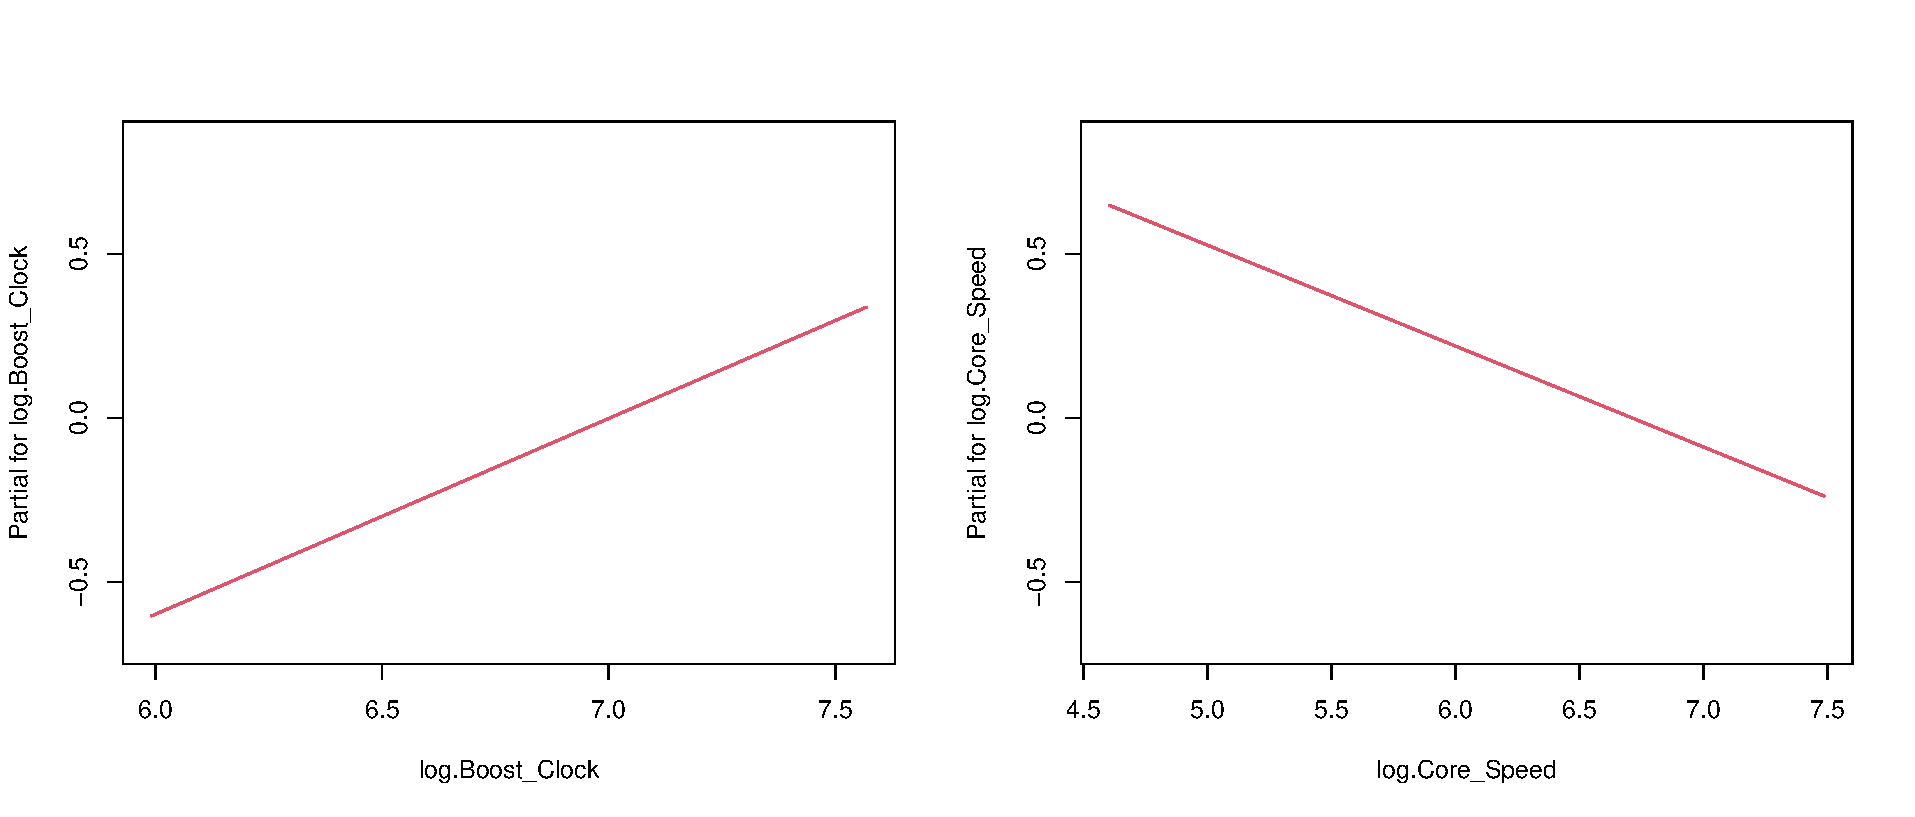
\includegraphics[keepaspectratio, width=1\textwidth, height=1\textheight]{LRM/Rplot3.pdf}
\end{figure}
\begin{figure}[H]
    \centering
    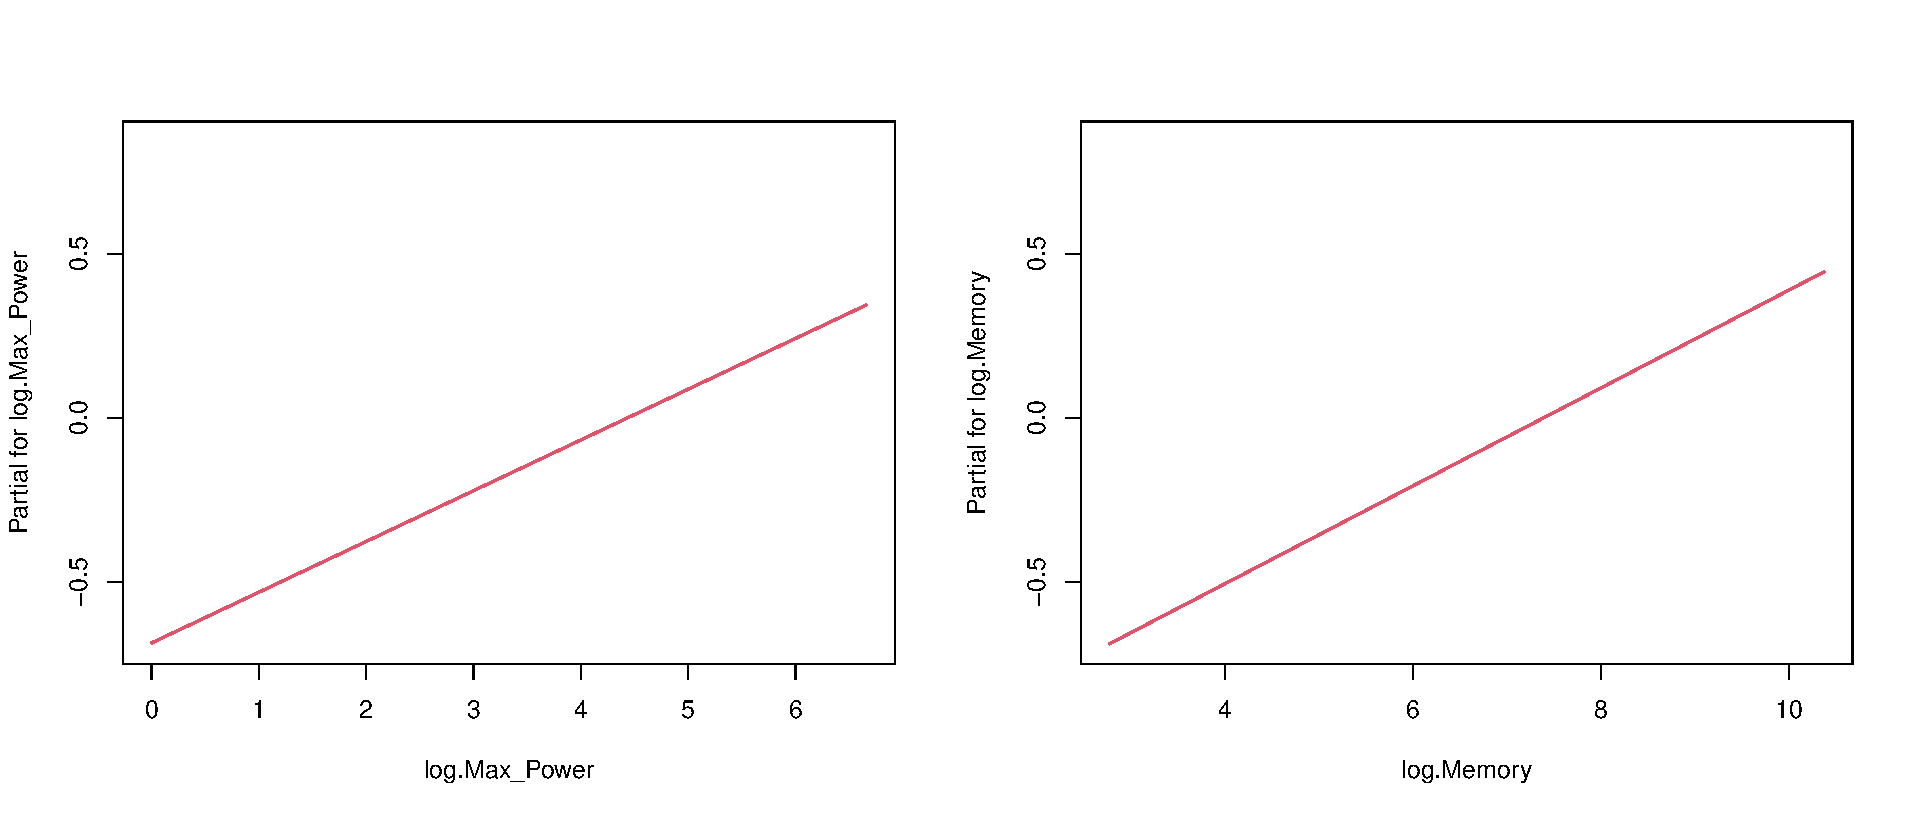
\includegraphics[keepaspectratio, width=1\textwidth, height=1\textheight]{LRM/Rplot4.pdf}
\end{figure}
\begin{figure}[H]
    \centering
    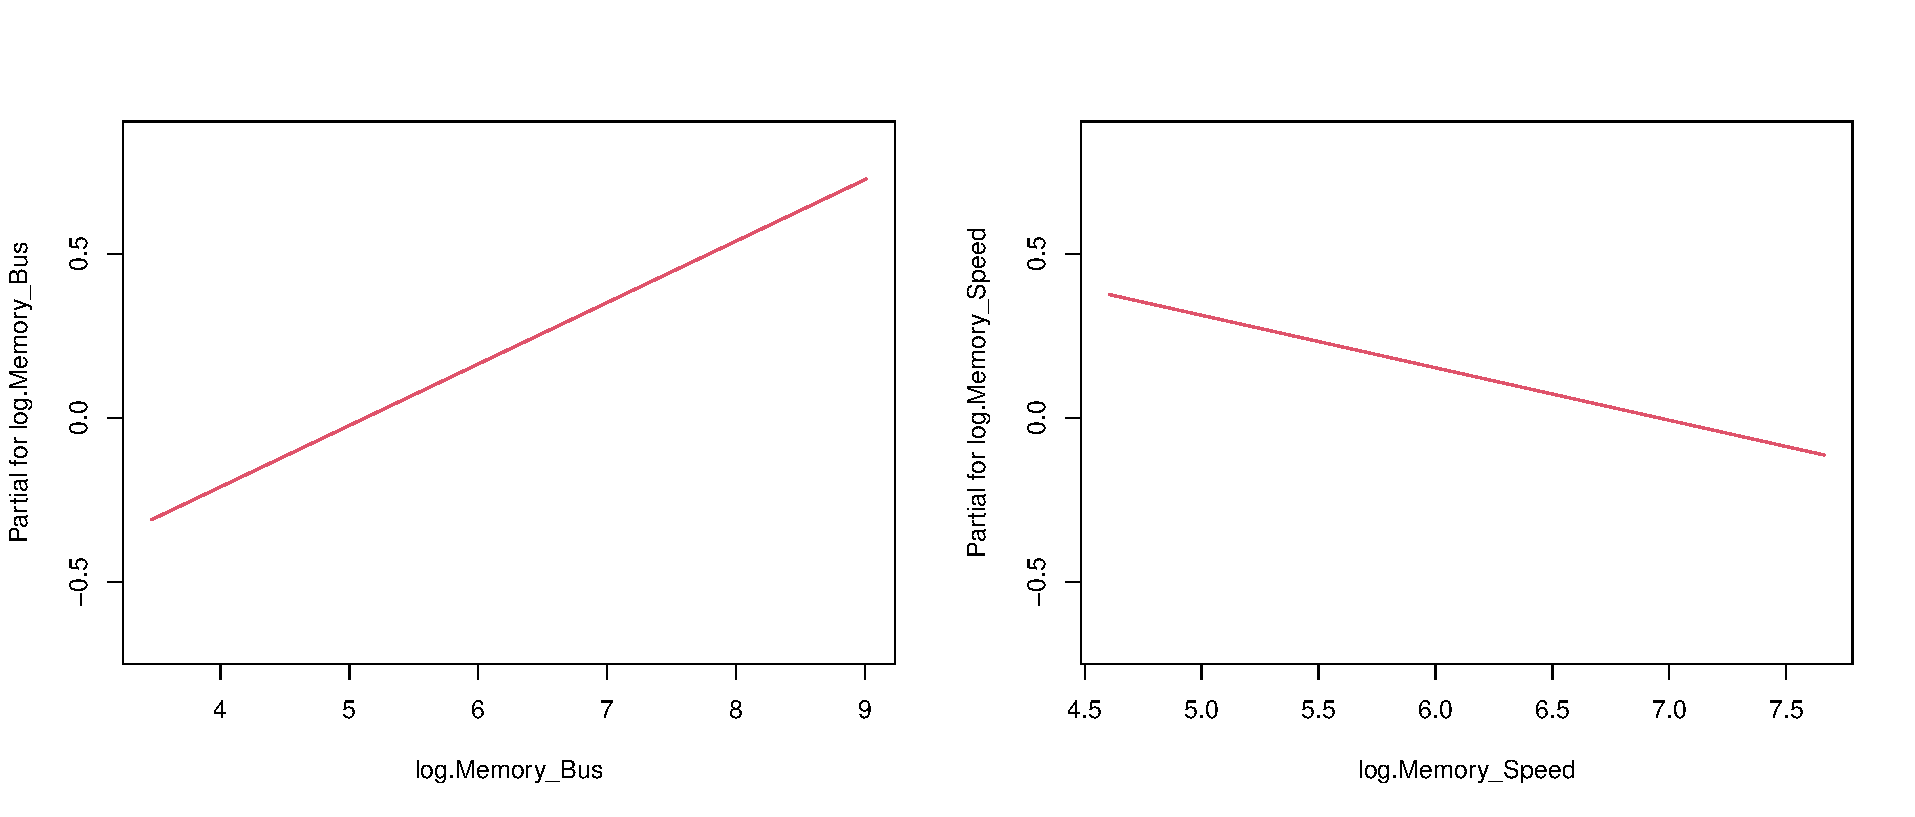
\includegraphics[keepaspectratio, width=1\textwidth, height=1\textheight]{LRM/Rplot5.pdf}
\end{figure}
\begin{figure}[H]
    \centering
    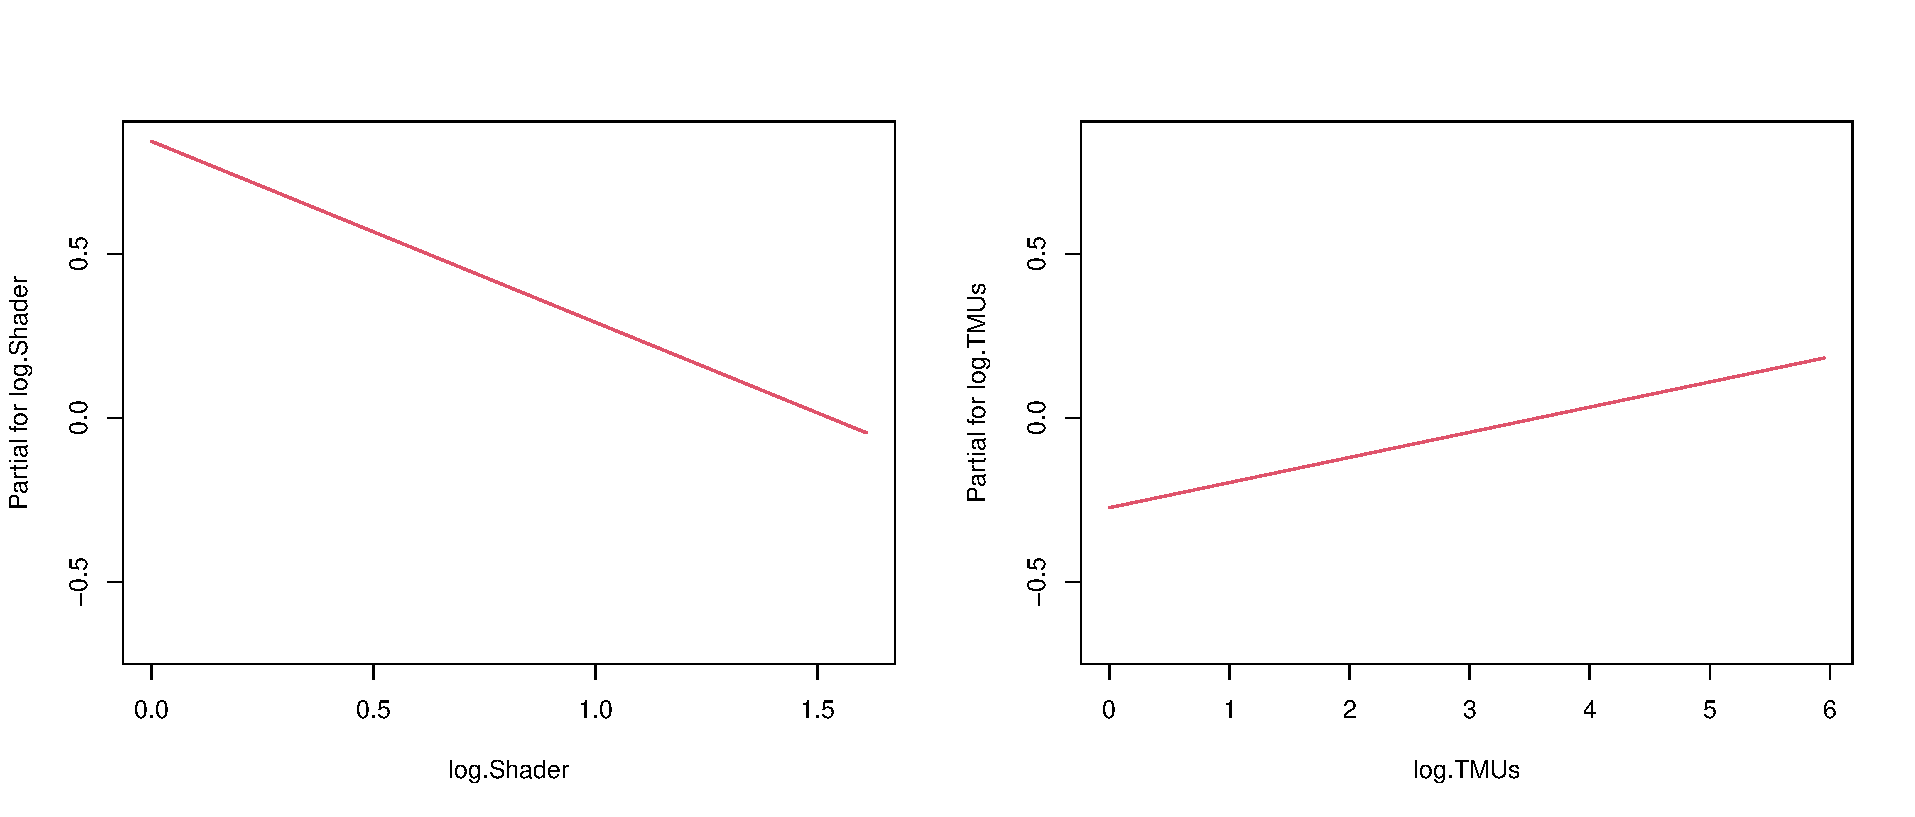
\includegraphics[keepaspectratio, width=1\textwidth, height=1\textheight]{LRM/Rplot6.pdf}
\end{figure}

\subsubsection{Graphs involving multiple variables}
First, we try a combination of price, accessible memory capacity and maximum power.
\begin{mdframed}[leftline=false,rightline=false,backgroundcolor=lightblue!10,nobreak=false]
    \begin{minted}[linenos,breaklines,breaksymbolleft=,obeytabs=true,tabsize=2]{R}
price.graph <-ggplot(df, aes(x = log.Release_Price, y = log.Memory, color = log.Max_Power)) + geom_point() + theme_classic()
price.graph <- price.graph + geom_smooth(method = "lm", col = "red")
price.graph
    \end{minted}
\end{mdframed}
\begin{figure}[H]
    \centering
    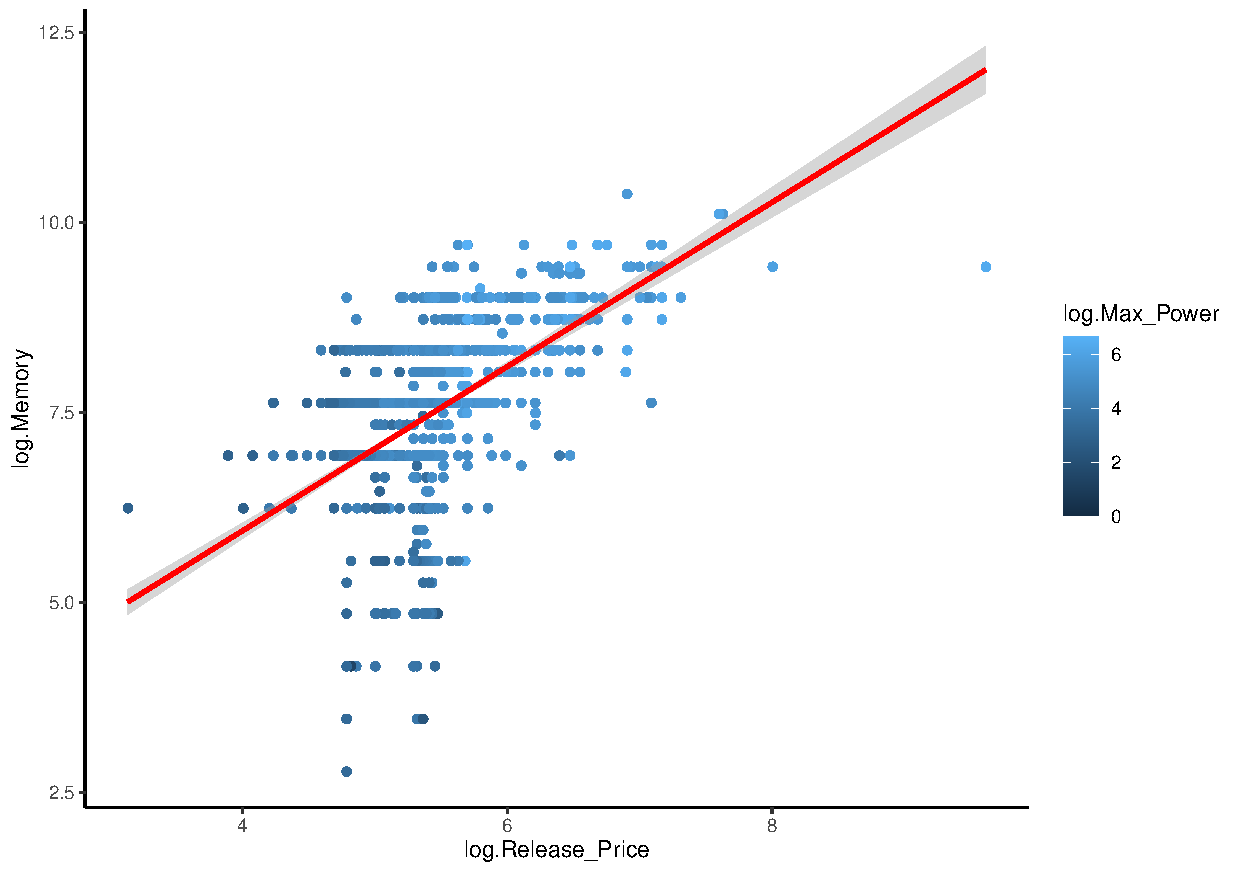
\includegraphics[keepaspectratio, width=1\textwidth, height=1\textheight]{LRM/Rplot7.pdf}
\end{figure}
Then we try a combination of price, boost clock speed and memory speed.
\begin{mdframed}[leftline=false,rightline=false,backgroundcolor=lightblue!10,nobreak=false]
    \begin{minted}[linenos,breaklines,breaksymbolleft=,obeytabs=true,tabsize=2]{R}
price_2.graph <-ggplot(df, aes(x = log.Release_Price, y = log.Boost_Clock, color = log.Memory_Speed)) + geom_point() + theme_classic()
price_2.graph <- price_2.graph + geom_smooth(method = "lm", col = "red")
price_2.graph
    \end{minted}
\end{mdframed}
\begin{figure}[H]
    \centering
    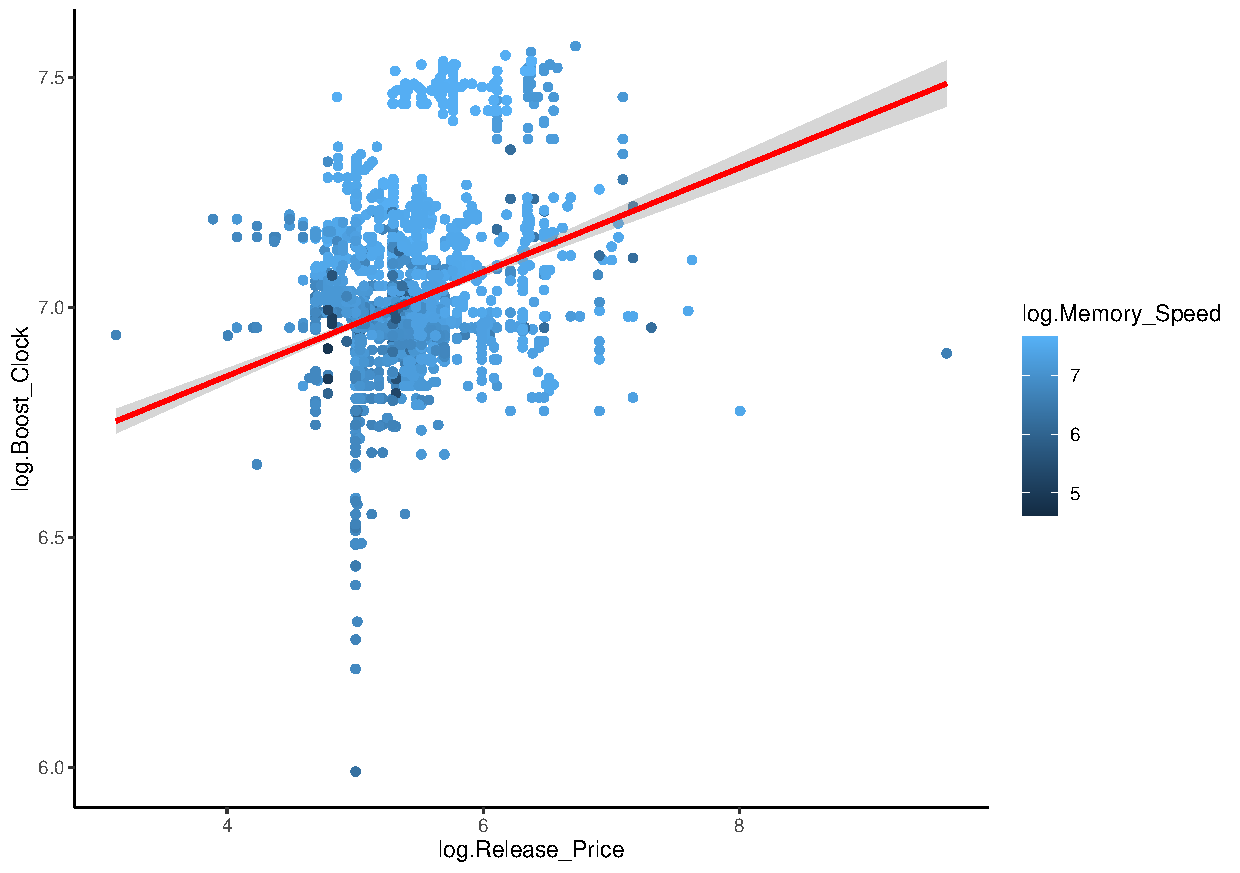
\includegraphics[keepaspectratio, width=1\textwidth, height=1\textheight]{LRM/Rplot8.pdf}
\end{figure}
Finally, we try a combination of price, core speed and the size of the data transmission channel inside the memory.
\begin{mdframed}[leftline=false,rightline=false,backgroundcolor=lightblue!10,nobreak=false]
    \begin{minted}[linenos,breaklines,breaksymbolleft=,obeytabs=true,tabsize=2]{R}
price_3.graph <-ggplot(df, aes(x = log.Release_Price, y = Core_Speed, color = log.Memory_Bus)) + geom_point() + theme_classic()
price_3.graph <- price_3.graph + geom_smooth(method = "lm", col = "red")
price_3.graph
    \end{minted}
\end{mdframed}
\begin{figure}[H]
    \centering
    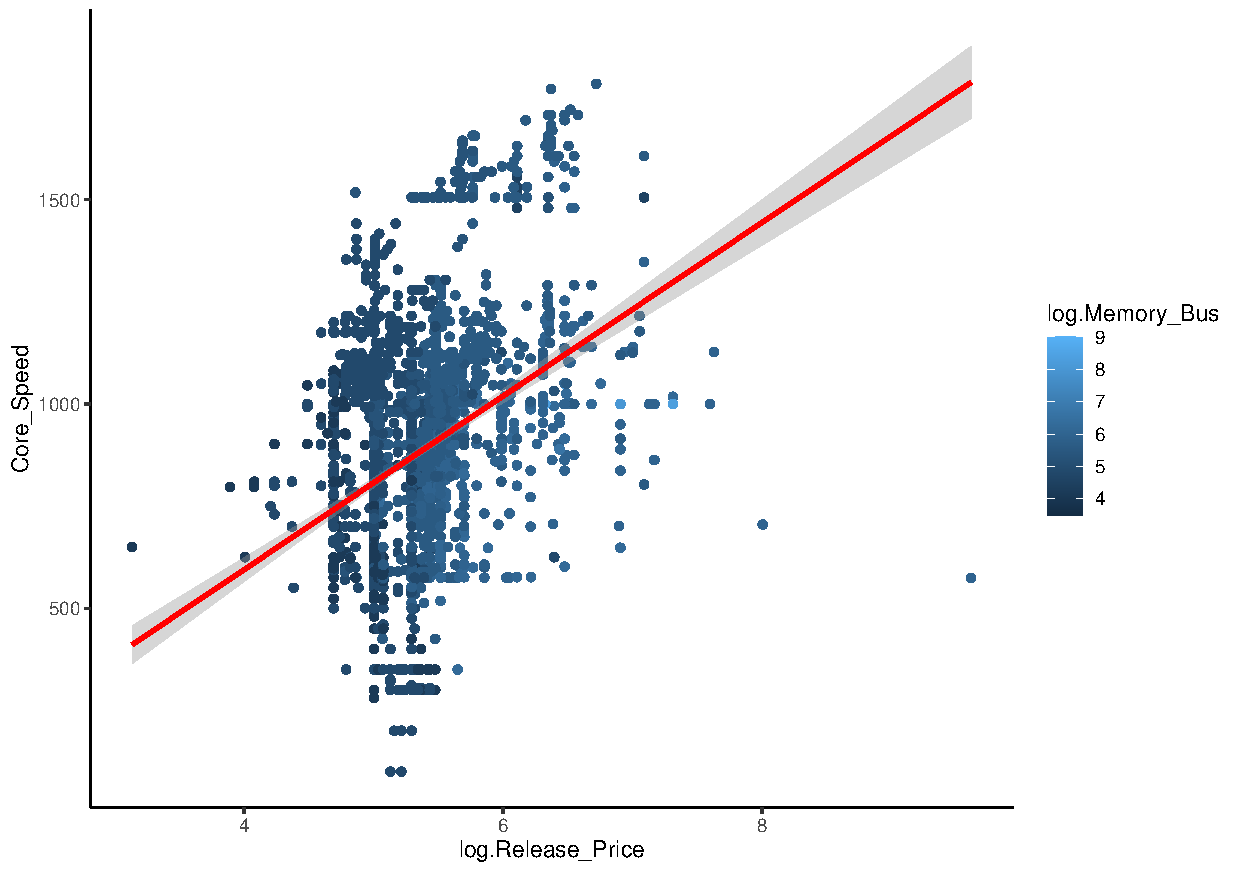
\includegraphics[keepaspectratio, width=1\textwidth, height=1\textheight]{LRM/Rplot9.pdf}
\end{figure}

\subsection{Model conclusion}
In the section above, we choose the linear regression model \verb|lmPrice|. According to this model, the estimated coefficient of
\begin{itemize}
    \item \verb|Boost_Clock|
    \item \verb|Max_Power|
    \item \verb|Memory|
    \item \verb|Memory_Bus|
    \item \verb|TMUs|
\end{itemize}
imply that these five variables will \textcolor{red}{increase} the \verb|Release_Price| of GPUs. Meanwhile, 
\begin{itemize}
    \item \verb|Core_Speed|
    \item \verb|Memory_Speed|
    \item \verb|Shader|
\end{itemize}
will \textcolor{mygreen}{decrease} the \verb|Release_Price| of GPUs due to their negative coefficients.

%%%%%%%%%%%%%%%%%%%%%%%%%%%%%%%%%%%%%%%%%%%%%%%%%%%%%%%%%%%%%%%%%%
\section{Fitting extra model}
\subsection{Fitting exponential model}
\subsubsection{Moore's law}
Moore's law is a term used to refer to the observation made by Gordon Moore in 1965 that the number of transistors in a dense integrated circuit (IC) \textbf{doubles} about (approximately) every two years. This aspect of technological progress is important as the capabilities of many digital electronic devices are strongly linked to Moore’s Law.\\\\
The observation is named after Gordon Moore, the co-founder of Fairchild Semiconductor and Intel (and former CEO of the latter), who in 1965 posited a doubling every year in the number of components per integrated circuit, and projected this rate of growth would continue for at least another decade. In 1975, looking forward to the next decade, he revised the forecast to doubling every two years, a compound annual growth rate (CAGR) of 41\%. While Moore did not use empirical evidence in forecasting that the historical trend would continue, his prediction held since 1975 and has since become known as a “law”.\\\\
As our large updated graph here shows, he was not only right about the next ten years but astonishingly the regularity he found is true for more than half a century now.
\begin{figure}[H]
    \centering
    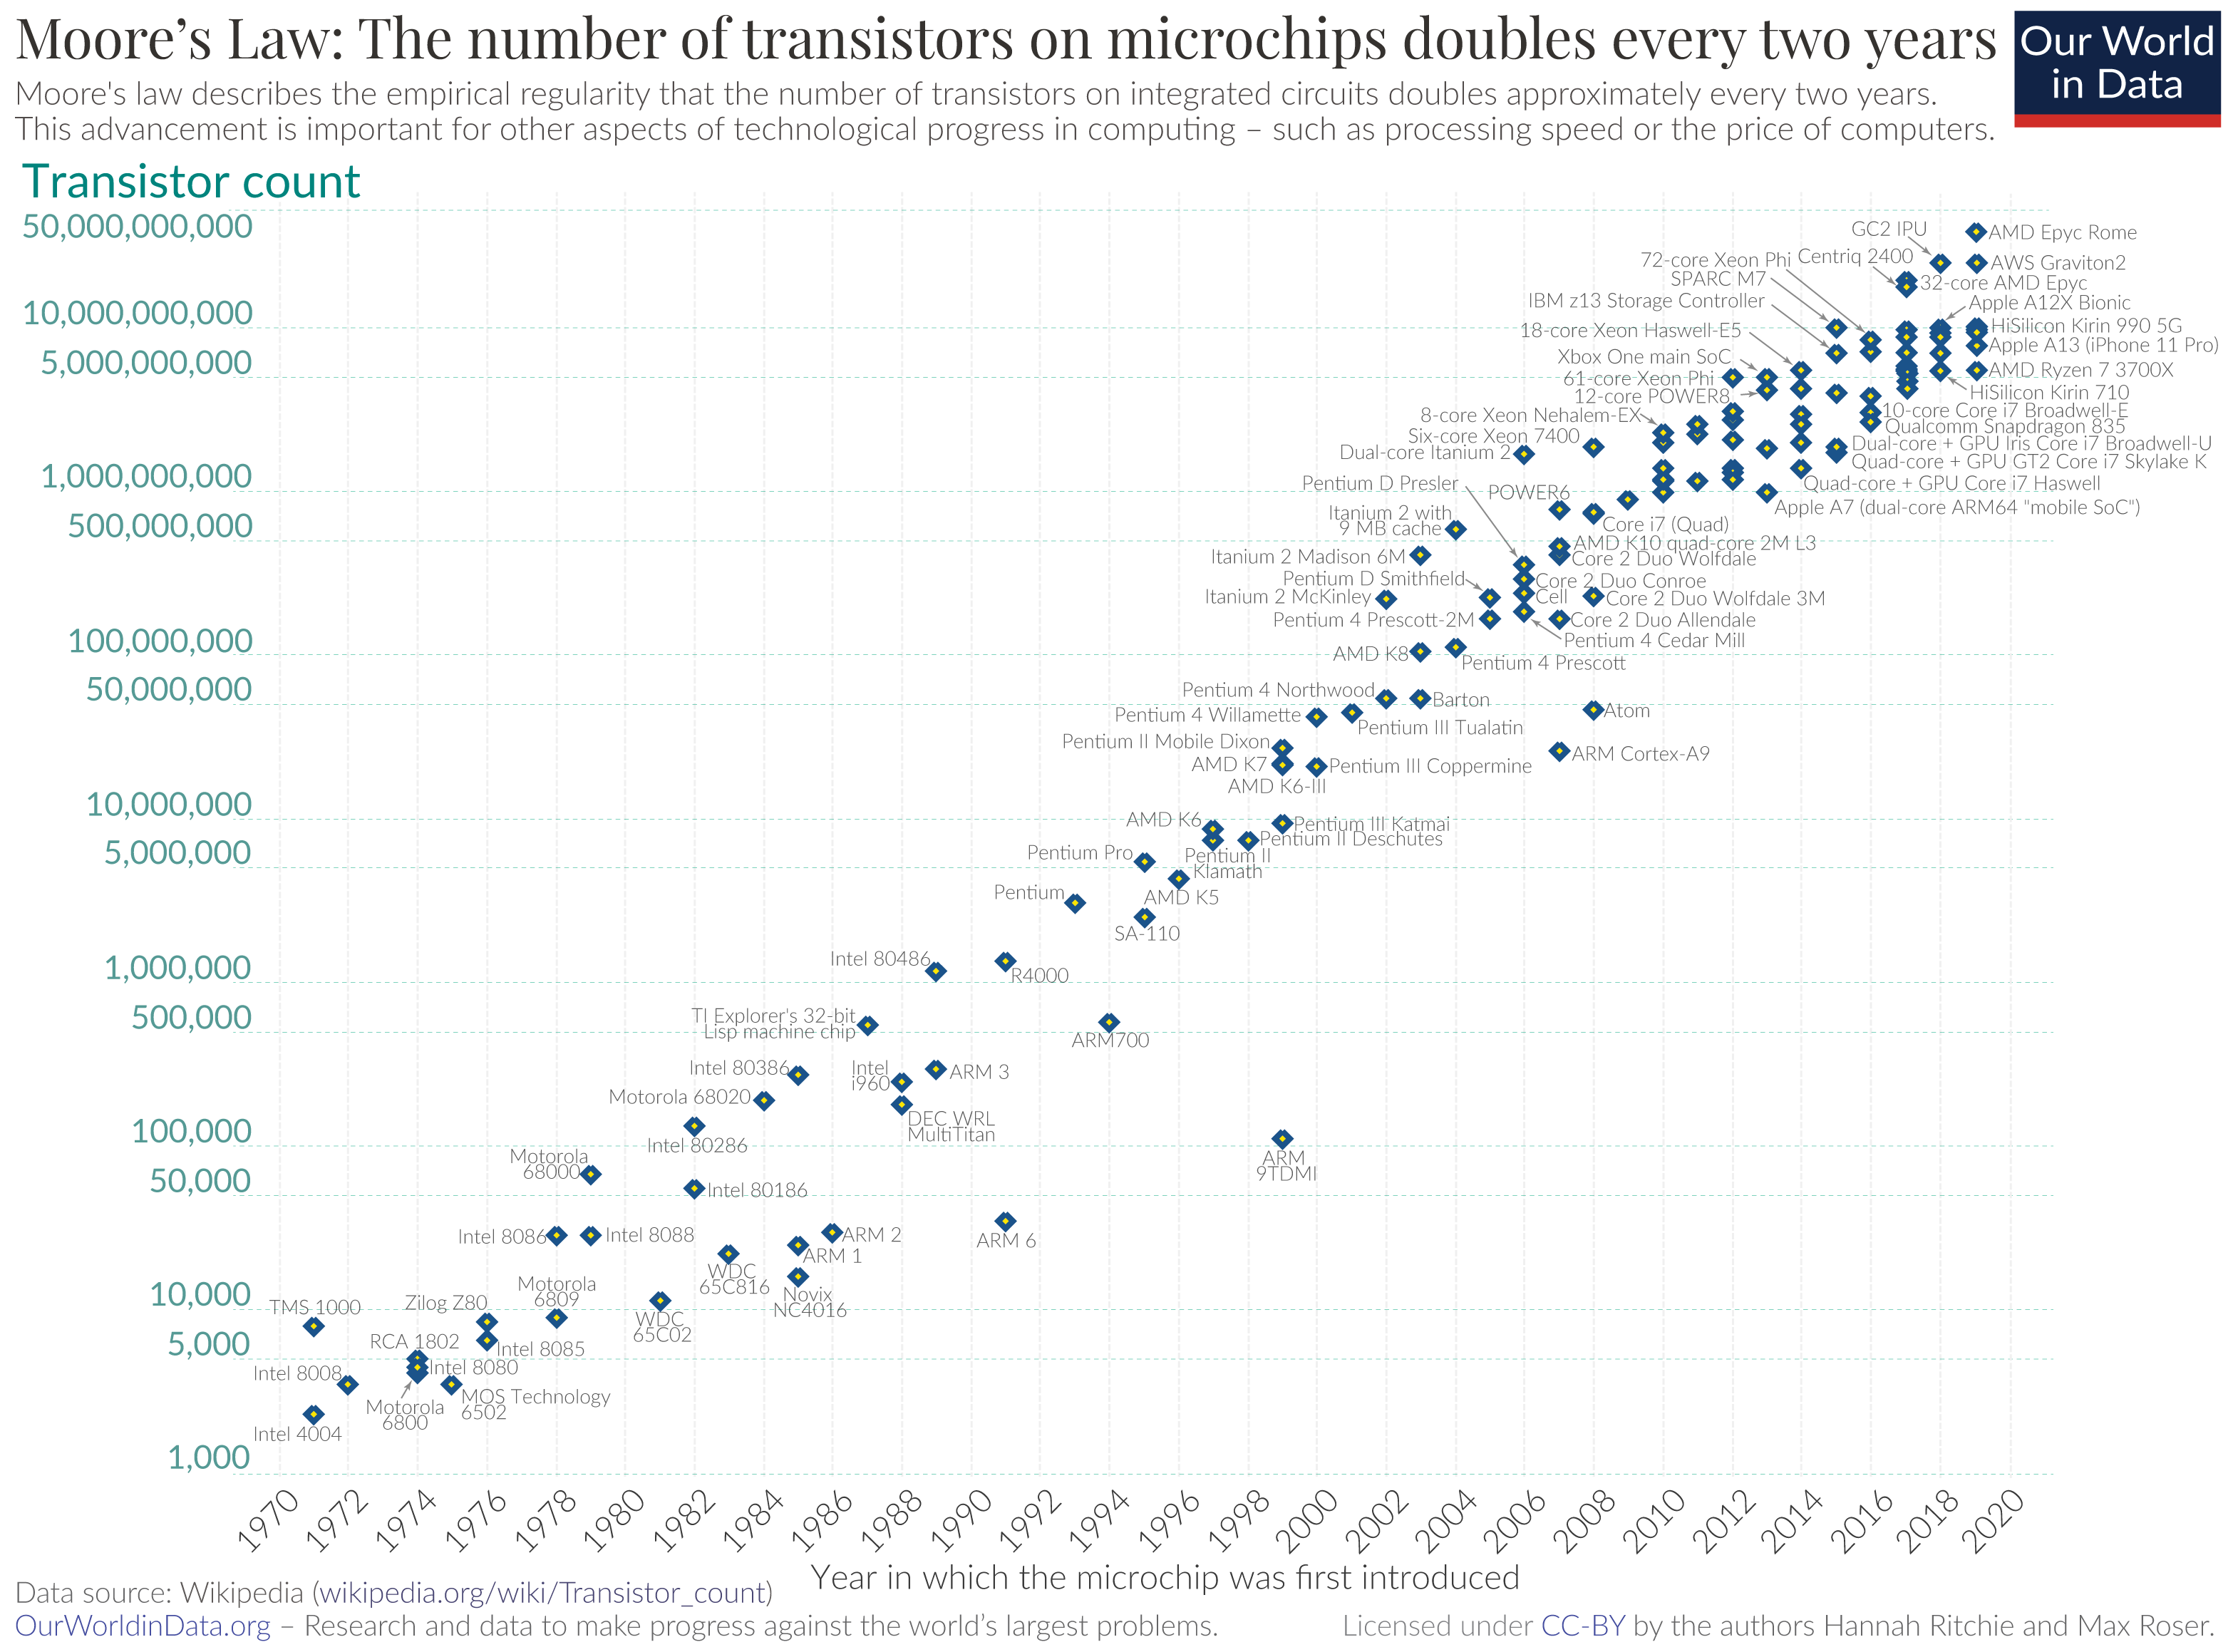
\includegraphics[keepaspectratio, width=1\textwidth, height=1\textheight]{EM/Moore_law.png}
\end{figure}
\subsubsection{Theoretic model}
Since our data is about the GPU, it also means about the circuit. Therefore, if the data is converted to logarithmic form, the graph, if Moore's law is correct, should be close to a straight line. In fact, the function representing the memory size calculated using Moore's law can be expressed as:
\begin{equation*}
    f(x)=y_{min}2^{\frac{x-x_{min}}{2}}
\end{equation*}
where:
\begin{itemize}
    \item $y_{min}$: Initial size of memory in MB.
    \item $x_{min}$: Initial year of dataset.
\end{itemize}
\subsubsection{Graphs}
Now we will plot a graph to see if the GPU's memory obeys Moore's law. First, we create 3 arrays:
\begin{itemize}
    \item \verb|year_arr|: This is an array of year values sorted in ascending order.
    \item \verb|memory_arr_mean|: This is an array of mean (average) memory capacity values grouped by year and sorted in ascending order.
    \item \verb|memory_arr_median|: This is an array of median memory capacity values grouped by year and sorted in ascending order.
\end{itemize}
\begin{mdframed}[leftline=false,rightline=false,backgroundcolor=lightblue!10,nobreak=false]
    \begin{minted}[linenos,breaklines,breaksymbolleft=,obeytabs=true,tabsize=2]{R}
year_arr <- unique(sort(strtoi(df$Release_Year)))

memory_arr_mean = data.frame(df %>% group_by(Release_Year) %>% summarise_at(vars(Memory), list(name = mean)))
memory_arr_mean = array(memory_arr_mean$name)

memory_arr_median = data.frame(df %>% group_by(Release_Year) %>% summarise_at(vars(Memory), list(name = median)))
memory_arr_median = array(memory_arr_median$name)
    \end{minted}
\end{mdframed}
Next we create two functions \verb|calculateMooresValue()| and \verb|exponentialCurve()|:

\begin{mdframed}[leftline=false,rightline=false,backgroundcolor=lightblue!10,nobreak=false]
    \begin{minted}[linenos,breaklines,breaksymbolleft=,obeytabs=true,tabsize=2]{R}
calculateMooresValue <- function(x, y_trans) {
  return(memory_arr_median[1] * 2**((x-y_trans)/2))
}

exponentialCurve <- function(x, a, b, c) {
  return(a*2**((x-c)*b))
}
    \end{minted}
\end{mdframed}
\begin{itemize}
    \item \verb|calculateMooresValue()|: The function $f(x)$ that we mentioned above. Used to calculate the theoretical value according to Moorse's law.
    \begin{itemize}
        \item Input: 
        \begin{itemize}
            \item \verb|x|: Current year.
            \item \verb|y_trans|: Start year (smallest year).
            \item \verb|memory_arr_median[1]|: Median value of start year.
        \end{itemize}
        \item Output:
        \begin{itemize}
            \item The value of the year's memory capacity is entered.
        \end{itemize}
    \end{itemize}
    \item \verb|exponentialCurve()|: Used to fit exponential curve to  our dataset.
    \begin{itemize}
        \item Input:
        \begin{itemize}
            \item \verb|x|: Current year.
            \item \verb|a|: Median value.
            \item \verb|b|: The coefficient corresponds to the factor $\dfrac{1}{2}$ in the $2^{\frac{1}{2}...}$ exponent of the formula $f(x)$.
            \item \verb|c|: Start year.
        \end{itemize}
        \item Output:
        \begin{itemize}
            \item The coordinate value of the $y$-axis of the function $f(x)$ according to our data set.
        \end{itemize}
    \end{itemize}
\end{itemize}
We use Python to find the triple variable \verb|a|, \verb|b| and \verb|c| because this language has very strong support libraries for fitting curves. Take a look \href{https://colab.research.google.com/drive/1ixVXEsUy2YtcCrayuPR6mmMf80pT92nh#scrollTo=ZXG4Ws3mTTNT}{here} again.
\begin{mdframed}[leftline=false,rightline=false,backgroundcolor=lightblue!10,nobreak=false]
    \begin{minted}[linenos,breaklines,breaksymbolleft=,obeytabs=true,tabsize=2]{Python}
popt, pcov = curve_fit(f=exponentialCurve,  xdata=year_arr, ydata=memory_arr_mean,  p0=(2, 0.5, 1998))
    \end{minted}
\end{mdframed}
\begin{itemize}
    \item \verb|popt|: Optimal values for the parameters, specifically here are \verb|a|, \verb|b| and \verb|c|.
    \item \verb|pcov|: The estimated covariance of \verb|popt|.
    \item \verb|f|: Our function $f(x)$.
    \item \verb|xdata|: $x$-coordinate data.
    \item \verb|ydata|: $y$-coordinate data.
    \item \verb|p0|: The initial guess for the fitting coefficients.
\end{itemize}
We check the returned values.
\begin{mdframed}[leftline=false,rightline=false,backgroundcolor=lightblue!10,nobreak=false]
    \begin{minted}[linenos,breaklines,breaksymbolleft=,obeytabs=true,tabsize=2]{Python}
print(popt)
    \end{minted}
\end{mdframed}
\begin{lstlisting}
 [1.04294249e+01 3.55525954e-01 1.99040139e+03]
\end{lstlisting}
These numbers mean:
\begin{itemize}
    \item \verb|a = 1.04294249e+01| 
    \item \verb|b = 3.55525954e-01| 
    \item \verb|c = 1.99040139e+03| 
\end{itemize}
Back to RStudio, we will build two models based on Moore's law and the above results.
\begin{mdframed}[leftline=false,rightline=false,backgroundcolor=lightblue!10,nobreak=false]
    \begin{minted}[linenos,breaklines,breaksymbolleft=,obeytabs=true,tabsize=2]{R}
y_pred_moore_law_teoretic = calculateMooresValue(year_arr, year_arr[1])
popt <- c(1.04294249e+01, 3.55525954e-01, 1.99040139e+03)
y_pred_moore_law_fitted = exponentialCurve(year_arr, popt[1], popt[2], popt[3])
    \end{minted}
\end{mdframed}
And then we built a graph to compare. For convenient drawing and manipulation, we create a new data frame \verb|df_extra| and store all the above values in it.
\begin{mdframed}[leftline=false,rightline=false,backgroundcolor=lightblue!10,nobreak=false]
    \begin{minted}[linenos,breaklines,breaksymbolleft=,obeytabs=true,tabsize=2]{R}
df_extra<-data.frame(Release_Year = year_arr, Memory_Mean = memory_arr_mean, Memory_Median = memory_arr_median, Moore_Teoretic = y_pred_moore_law_teoretic, Moore_Fitted = y_pred_moore_law_fitted)

ggplot(df_extra, aes(x = Release_Year)) +  theme_classic() + 
  scale_x_continuous(breaks = scales::pretty_breaks(n = 20)) +
  theme(legend.position='bottom', plot.title = element_text(hjust = 0.5)) +
  xlab("Year") + ylab("GPU Memory") + labs(colour="") + 
  ggtitle("GPU Memory vs Year of Release (logaritmic scale)") + 
  geom_line(aes(y = log(Memory_Mean), colour = "Mean")) + 
  geom_line(aes(y = log(Memory_Median), colour = "Median")) +
  geom_line(aes(y = log(Moore_Teoretic), colour = "Moore's law teoretic")) +
  geom_line(aes(y = log(Moore_Fitted), colour = "Moore's law fitted")) 
    \end{minted}
\end{mdframed}
\begin{figure}[H]
    \centering
    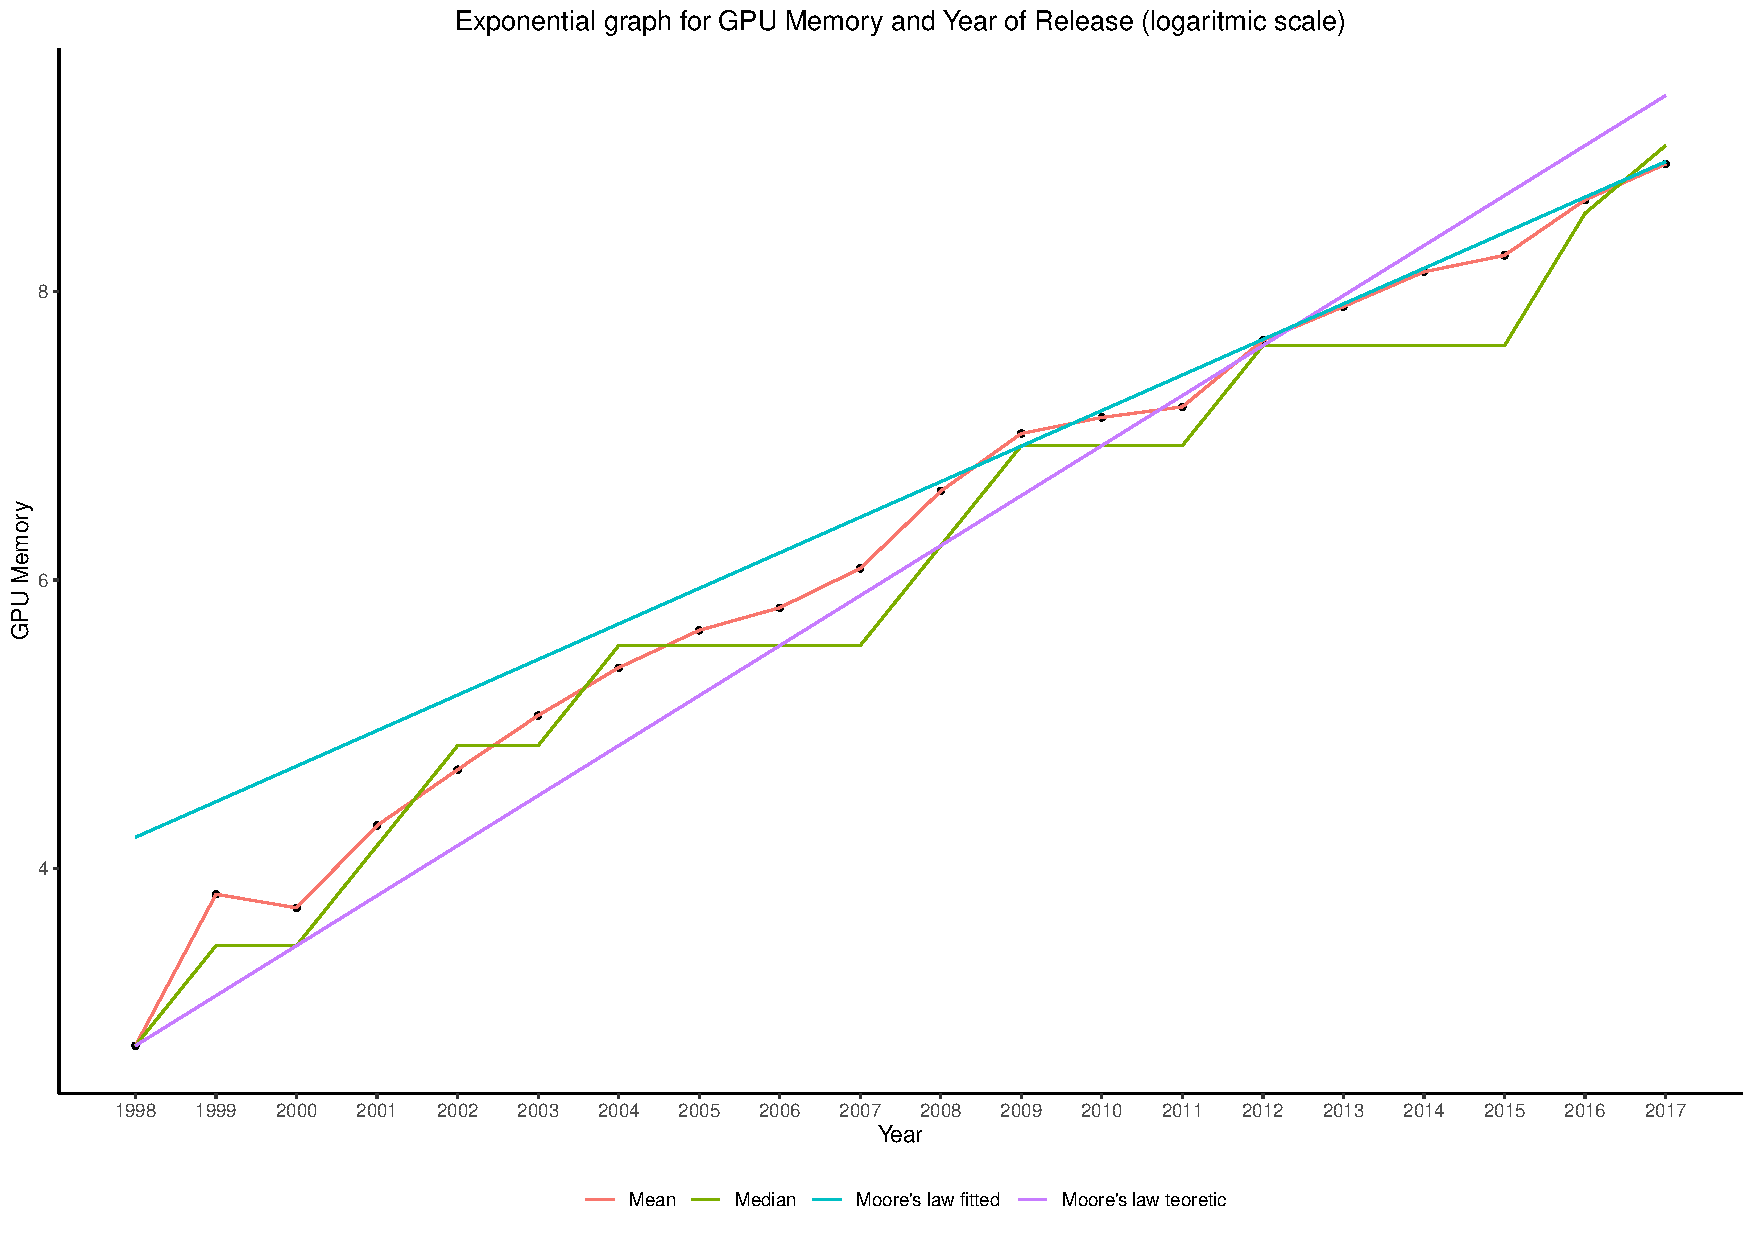
\includegraphics[keepaspectratio, width=1\textwidth, height=1\textheight]{EM/compared_graph.pdf}
\end{figure}
As we can see, mean size [\textcolor{red}{red line}] of GPUs memory tends to follow teoretic Moore's law curve [\textcolor{purple}{purple line}] but not ideally. We need to do something to better fit the dataset [\textcolor{cyan}{cyan line}]. Therefore, we will try with the polynomial model in the next section. Besides, we also draw a graph to the original scale for easy comparison with the polynomial model.
\begin{figure}[H]
    \centering
    \includegraphics[keepaspectratio, width=1\textwidth, height=1\textheight]{EM/exp_graph.pdf}
\end{figure}
%%%%%%%%%%%%%%%%%%%%%%%%%%%%%%%%%%%%%%%%%%%%%%%%%%%%%%%%%%%%%%%%%%
\subsection{Fitting polynomial regression model}
In this section, we build a polynomial regression model to compare with other models. We will focus only on the average value of the memory.
\subsubsection{Constructing quadratic polynomial regression}
A quadratic regression is the process of finding the equation of the parabola that best fits a set of data. As a result, we get an equation of the form:
\begin{equation*}
    y=ax^2+bx+c
\end{equation*}
where:
\begin{itemize}
    \item $a \neq 0$.
    \item $y$: Size of memory in MB.
    \item $x$: Year.
\end{itemize}
\begin{mdframed}[leftline=false,rightline=false,backgroundcolor=lightblue!10,nobreak=false]
    \begin{minted}[linenos,breaklines,breaksymbolleft=,obeytabs=true,tabsize=2]{R}
poly_2_mean <- lm(Memory_Mean ~ Release_Year + I(Release_Year^2), data=df_extra)
summary(poly_2_mean)
    \end{minted}
\end{mdframed}
\begin{lstlisting}
 Call:
 lm(formula = log(Memory_Mean) ~ Release_Year + I(Release_Year^2), 
     data = df_extra)

 Residuals:
      Min       1Q   Median       3Q      Max 
 -0.31983 -0.11978  0.01628  0.08554  0.33658 

 Coefficients:
                     Estimate Std. Error t value Pr(>|t|)    
 (Intercept)       -2.159e+04  4.736e+03  -4.559 0.000278 ***
 Release_Year       2.122e+01  4.719e+00   4.497 0.000318 ***
 I(Release_Year^2) -5.211e-03  1.175e-03  -4.434 0.000364 ***
 ---
 Signif. codes:  0 '***' 0.001 '**' 0.01 '*' 0.05 '.' 0.1 ' ' 1

 Residual standard error: 0.1557 on 17 degrees of freedom
 Multiple R-squared:  0.9932,	Adjusted R-squared:  0.9924 
 F-statistic:  1241 on 2 and 17 DF,  p-value: < 2.2e-16
\end{lstlisting}
Let's take a look at the coefficients of the above model.
\begin{mdframed}[leftline=false,rightline=false,backgroundcolor=lightblue!10,nobreak=false]
    \begin{minted}[linenos,breaklines,breaksymbolleft=,obeytabs=true,tabsize=2]{R}
coef(poly_2_mean)
    \end{minted}
\end{mdframed}
\begin{lstlisting}
       (Intercept)      Release_Year I(Release_Year^2) 
      1.273072e+08     -1.271265e+05      3.173648e+01 
\end{lstlisting}
Looks good, now we are going to predict the amount of memory (value on the y-axis) from the model.
\begin{mdframed}[leftline=false,rightline=false,backgroundcolor=lightblue!10,nobreak=false]
    \begin{minted}[linenos,breaklines,breaksymbolleft=,obeytabs=true,tabsize=2]{R}
year_df <- data.frame(Release_Year = year_arr)
y_pred_lin_reg_2 <- predict(poly_2_mean, year_df, type="response")
    \end{minted}
\end{mdframed}
And then we save these values to the data frame.
\begin{mdframed}[leftline=false,rightline=false,backgroundcolor=lightblue!10,nobreak=false]
    \begin{minted}[linenos,breaklines,breaksymbolleft=,obeytabs=true,tabsize=2]{R}
df_extra$Y_pred_lin_reg_2 <- y_pred_lin_reg_2
    \end{minted}
\end{mdframed}


\subsubsection{Constructing cubic polynomial regression}\
Like a quadratic polynomial, a cubic polynomial is a polynomial of the form:
\begin{equation*}
    y=ax^3+bx^2+cx+d
\end{equation*}
where:
\begin{itemize}
    \item $a \neq 0$.
    \item $y$: Size of memory in MB.
    \item $x$: Year.
\end{itemize}
\begin{mdframed}[leftline=false,rightline=false,backgroundcolor=lightblue!10,nobreak=false]
    \begin{minted}[linenos,breaklines,breaksymbolleft=,obeytabs=true,tabsize=2]{R}
poly_3_mean <- lm(Memory_Mean ~ Release_Year + I(Release_Year^2) + I(Release_Year^3), data=df_e)
summary(poly_3_mean)
    \end{minted}
\end{mdframed}
\begin{lstlisting}
 Call:
 lm(formula = Memory_Mean ~ Release_Year + I(Release_Year^2) + 
     I(Release_Year^3), data = df_extra)

 Residuals:
     Min      1Q  Median      3Q     Max 
 -670.09 -344.06   87.56  286.96 1041.90 

 Coefficients: (1 not defined because of singularities)
                     Estimate Std. Error t value Pr(>|t|)    
 (Intercept)        1.273e+08  1.337e+07   9.524 3.15e-08 ***
 Release_Year      -1.271e+05  1.332e+04  -9.546 3.05e-08 ***
 I(Release_Year^2)  3.174e+01  3.317e+00   9.568 2.95e-08 ***
 I(Release_Year^3)         NA         NA      NA       NA    
 ---
 Signif. codes:  0 '***' 0.001 '**' 0.01 '*' 0.05 '.' 0.1 ' ' 1

 Residual standard error: 439.5 on 17 degrees of freedom
 Multiple R-squared:  0.9584,	Adjusted R-squared:  0.9535 
 F-statistic:   196 on 2 and 17 DF,  p-value: 1.815e-12
\end{lstlisting}
It seems that in the 3rd degree polynomial model, there is an error that the two or more independent variables are perfectly collinear.Indeed, the error \texttt{not defined because of singularities} will occur due to strong correlation between independent variables. And if this error occurs we will not be able to find the predicted $y$ value because one of the coefficients of the model is missing.\\\\
Therefore, to be able to run this model, we use Python to get the coefficients for the model. Check \href{https://colab.research.google.com/drive/1ixVXEsUy2YtcCrayuPR6mmMf80pT92nh#scrollTo=BNuGVxNW7V_B}{here}.
\begin{mdframed}[leftline=false,rightline=false,backgroundcolor=lightblue!10,nobreak=false]
    \begin{minted}[linenos,breaklines,breaksymbolleft=,obeytabs=true,tabsize=2]{Python}
print(lin_reg_3.intercept_)
    \end{minted}
\end{mdframed}
\begin{lstlisting}
 -17128661108.085476
\end{lstlisting}
\begin{mdframed}[leftline=false,rightline=false,backgroundcolor=lightblue!10,nobreak=false]
    \begin{minted}[linenos,breaklines,breaksymbolleft=,obeytabs=true,tabsize=2]{Python}
print(lin_reg_3.coef_)
    \end{minted}
\end{mdframed}
\begin{lstlisting}
 [ 2.56615577e+07 -1.28150909e+04  2.13323868e+00]
\end{lstlisting}
After obtaining the coefficient values, we change them with the corresponding values existing in the model.
\begin{mdframed}[leftline=false,rightline=false,backgroundcolor=lightblue!10,nobreak=false]
    \begin{minted}[linenos,breaklines,breaksymbolleft=,obeytabs=true,tabsize=2]{R}
poly_3_mean$coefficients[1:4] <- c(-17128661108.085476, 2.56615577e+07, -1.28150909e+04,  2.13323868e+00)
poly_3_mean$rank <- c(4)
    \end{minted}
\end{mdframed}
Note that because in the model when the coefficients have not been changed, there is an \verb|NA| value for the coefficient, so the rank of the model will then be missing by one unit. Therefore, when changing the coefficient, it is necessary to change the rank of the new model (plus 1 unit). We already know the rank factor was 3 before, so we just need to replace 3 by 4.\\\\
We can now guess the $y$-axis value based on the model.

\begin{mdframed}[leftline=false,rightline=false,backgroundcolor=lightblue!10,nobreak=false]
    \begin{minted}[linenos,breaklines,breaksymbolleft=,obeytabs=true,tabsize=2]{R}
y_pred_lin_reg_3 <- predict(poly_3_mean, year_df, type="response")
    \end{minted}
\end{mdframed}
Then save the predicted values to the data frame \verb|df_extra|.
\begin{mdframed}[leftline=false,rightline=false,backgroundcolor=lightblue!10,nobreak=false]
    \begin{minted}[linenos,breaklines,breaksymbolleft=,obeytabs=true,tabsize=2]{R}
df_extra$Y_pred_lin_reg_3 <- y_pred_lin_reg_3
    \end{minted}
\end{mdframed}


\subsubsection{Graphs}
\begin{mdframed}[leftline=false,rightline=false,backgroundcolor=lightblue!10,nobreak=false]
    \begin{minted}[linenos,breaklines,breaksymbolleft=,obeytabs=true,tabsize=2]{R}
ggplot(df_extra, aes(x = Release_Year, y = log(Memory_Mean))) +  theme_classic() +
  scale_x_continuous(breaks = scales::pretty_breaks(n = 20)) +
  theme(legend.position='bottom', plot.title = element_text(hjust = 0.5)) +
  xlab("Year") + ylab("GPU Memory") + labs(colour="") + 
  ggtitle("Polynomial graph for GPU Memory and Year of Release (logaritmic scale)") + 
  geom_line(aes(y = y_pred_lin_reg_2, colour = "2nd degree polynomial"), n=1000) + 
  geom_line(aes(y = y_pred_lin_reg_3, colour = "3rd degree polynomial"), n=1000) +
  geom_line(aes(y = Moore_Teoretic, colour = "Moore's law teoretic"), n=1000) +
  geom_line(aes(y = Moore_Fitted, colour = "Moore's law fitted"), n=1000) 
    \end{minted}
\end{mdframed}
\begin{figure}[H]
    \centering
    \includegraphics[keepaspectratio, width=1\textwidth, height=1\textheight]{EM/poly.pdf}
\end{figure}
The 2nd degree polynomial model [\textcolor{red}{red line}] and the 3rd degree polynomial model  [\textcolor{mygreen}{green line}] are shown in the figure above. Based on that, we can see that this model is better than the exponential model. Can be verified \href{https://colab.research.google.com/drive/1ixVXEsUy2YtcCrayuPR6mmMf80pT92nh#scrollTo=vRHmN6RtiXz5}{here} or in the figure below. Note that Mean and Median are from the exponential model.\\\\
If we combine the two models above, we get the following figure.
\begin{mdframed}[leftline=false,rightline=false,backgroundcolor=lightblue!10,nobreak=false]
    \begin{minted}[linenos,breaklines,breaksymbolleft=,obeytabs=true,tabsize=2]{R}
ggplot(df_extra, aes(x = Release_Year, y = log(Memory_Mean))) +  theme_classic() +
  scale_x_continuous(breaks = scales::pretty_breaks(n = 20)) +
  theme(legend.position='bottom', plot.title = element_text(hjust = 0.5)) +
  xlab("Year") + ylab("GPU Memory") + labs(colour="") + 
  ggtitle("Exponential model vs Polynomial model") + 
  geom_line(aes(y = y_pred_lin_reg_2, colour = "2nd degree polynomial"), n=1000) + 
  geom_line(aes(y = y_pred_lin_reg_3, colour = "3rd degree polynomial"), n=1000) +
  geom_line(aes(y = Moore_Teoretic, colour = "Moore's law teoretic"), n=1000) +
  geom_line(aes(y = Moore_Fitted, colour = "Moore's law fitted"), n=1000) +
  geom_line(aes(y = Memory_Mean, colour = "Mean"), n=1000) + 
  geom_line(aes(y = Memory_Median, colour = "Median"), n=1000) 
    \end{minted}
\end{mdframed}
\begin{figure}[H]
    \centering
    \includegraphics[keepaspectratio, width=1\textwidth, height=1\textheight]{EM/exp_poly.pdf}
\end{figure}
%%%%%%%%%%%%%%%%%%%%%%%%%%%%%%%%%%%%%%%%%%%%%%%%%%%%%%%%%%%%%%%%%%

\section{Prediction}
In this section we will use our (linear regression) model to forecast the prices of several GPU models.
\subsection{From dataset}
\begin{itemize}
    \item \textbf{Case 1}
    \begin{itemize}
        \item \verb|Boost_Clock = mean(Boost_Clock)| 
        \item \verb|Core_Speed = mean(Core_Speed)|
        \item \verb|Max_Power = mean(Max_Power)|
        \item \verb|Memory = mean(Memory)|
        \item \verb|Memory_Bus = mean(Memory_Bus)|
        \item \verb|Memory_Speed = mean(Memory_Speed)|
        \item \verb|Shader = mean(Shader)|
        \item \verb|TMUs = mean(TMUs)|
    \end{itemize}
    
    \item \textbf{Case 2}
    \begin{itemize}
        \item \verb|Boost_Clock = median(Boost_Clock)| 
        \item \verb|Core_Speed = median(Core_Speed)|
        \item \verb|Max_Power = median(Max_Power)|
        \item \verb|Memory = median(Memory)|
        \item \verb|Memory_Bus = median(Memory_Bus)|
        \item \verb|Memory_Speed = median(Memory_Speed)|
        \item \verb|Shader = median(Shader)|
        \item \verb|TMUs = median(TMUs)|
    \end{itemize}
    
    \item \textbf{Case 3}
    \begin{itemize}
        \item \verb|Boost_Clock = max(Boost_Clock)| 
        \item \verb|Core_Speed = max(Core_Speed)|
        \item \verb|Max_Power = max(Max_Power)|
        \item \verb|Memory = max(Memory)|
        \item \verb|Memory_Bus = max(Memory_Bus)|
        \item \verb|Memory_Speed = max(Memory_Speed)|
        \item \verb|Shader = max(Shader)|
        \item \verb|TMUs = max(TMUs)|
    \end{itemize}
\end{itemize}
For the purpose of predicting the GPU prices in the 3 specific cases above:
\begin{itemize}
    \item \textbf{Step 1}: Create a data frame called \verb|predict_Data| containing 3 observations of 8 independent variables (as listed above): \texttt{Boost\_Clock, Core\_Speed, Max\_Power, Memory, Memory\_Bus, Memory\_Speed, Shader, TMUs}.
    \item \textbf{Step 2}: Call the \verb|predict()| function with the following syntax:
    \begin{center}
        \verb|predict(object, newdata, interval, level=0.95)|
    \end{center}
    where:
    \begin{itemize}
        \item \verb|object|: A model object for which predictions are desired. We will call our \verb|lmPrice| model.
        \item \verb|newdata|: The input data to predict the values.
        \item \verb|interval=c("none", "confidence", "prediction")|: type of interval calculation.
        \item \verb|level|: The confidence level. By default, this parameter equals to 0.95. 
    \end{itemize}
\end{itemize}

\begin{mdframed}[leftline=false,rightline=false,backgroundcolor=lightblue!10,nobreak=false]
    \begin{minted}[linenos,breaklines,breaksymbolleft=,obeytabs=true,tabsize=2]{R}
predict_Data = data.frame(
  log.Boost_Clock = c(mean(df[, 'log.Boost_Clock']), median(df[, 'log.Boost_Clock']), max(df[, 'log.Boost_Clock'])),
  log.Core_Speed = c(mean(df[, 'log.Core_Speed']), median(df[, 'log.Core_Speed']), max(df[, 'log.Core_Speed'])),
  log.Max_Power = c(mean(df[, 'log.Max_Power']), median(df[, 'log.Max_Power']), max(df[, 'log.Max_Power'])),
  log.Memory = c(mean(df[, 'log.Memory']), median(df[, 'log.Memory']), max(df[, 'log.Memory'])),
  log.Memory_Bus = c(mean(df[, 'log.Memory_Bus']), median(df[, 'log.Memory_Bus']), max(df[, 'log.Memory_Bus'])),
  log.Memory_Speed = c(mean(df[, 'log.Memory_Speed']), median(df[, 'log.Memory_Speed']), max(df[, 'log.Memory_Speed'])),
  log.Shader = c(mean(df[, 'log.Shader']), median(df[, 'log.Shader']), max(df[, 'log.Shader'])),
  log.TMUs = c(mean(df[, 'log.TMUs']), median(df[, 'log.TMUs']), max(df[, 'log.TMUs']))
)

predict(lmPrice, predict_Data, interval = "confidence", level = 0.95)
    \end{minted}
\end{mdframed}
\begin{figure}[H]
    \centering
    \includegraphics[keepaspectratio, width=1\textwidth, height=1\textheight]{Predict/1.png}
\end{figure}
\begin{lstlisting}
        fit      lwr      upr
 1 5.341435 5.330881 5.351988
 2 5.281895 5.265958 5.297833
 3 6.981385 6.882778 7.079993
\end{lstlisting}
We can use the \verb|exp()| function to invert the logarithm to get the original value.
\begin{mdframed}[leftline=false,rightline=false,backgroundcolor=lightblue!10,nobreak=false]
    \begin{minted}[linenos,breaklines,breaksymbolleft=,obeytabs=true,tabsize=2]{R}
exp(predict(lmPrice, predict_Data, interval = "confidence", level = 0.95))
    \end{minted}
\end{mdframed}
\begin{lstlisting}
         fit      lwr       upr
 1  208.8121 206.6200  211.0275
 2  196.7424 193.6316  199.9032
 3 1076.4082 975.3316 1187.9597
\end{lstlisting}
\begin{itemize}
    \item \textbf{Case 1}: The GPU's price is around \$208.8121  (from \$206.6200 to \$211.0275).
    \item \textbf{Case 2}: The GPU's price is around \$196.7424  (from \$193.6316 to \$199.9032).
    \item \textbf{Case 3}: The GPU's price is around \$1076.4082  (from \$975.3316 to \$1187.9597).
\end{itemize}

\subsection{From real life}
We try to predict the price of an Nvidia RTX 3090. Based on the specifications described \href{https://www.techpowerup.com/gpu-specs/geforce-rtx-3090.c3622}{here}, we feed the data into the \verb|lmPrice| model to predict the price.
\begin{mdframed}[leftline=false,rightline=false,backgroundcolor=lightblue!10,nobreak=false]
    \begin{minted}[linenos,breaklines,breaksymbolleft=,obeytabs=true,tabsize=2]{R}
spec_RTX_3090 = data.frame(
  log.Boost_Clock = log(1695),
  log.Core_Speed = log(1395),
  log.Max_Power = log(350),
  log.Memory = log(24576),
  log.Memory_Bus = log(384),
  log.Memory_Speed = log(1219),
  log.Shader = log(10496),
  log.TMUs =  log(328)
)

exp(predict(lmPrice, spec_RTX_3090, interval = "confidence", level = 0.95))
    \end{minted}
\end{mdframed}

\begin{lstlisting}
       fit     lwr      upr
 1 8.13446 4.39761 15.04668
\end{lstlisting}
From the above results, we get a pretty bad result. Due to the fact that a new RTX 3090 has a MSRP (Manufacturer's Suggested Retail Price) price announced by Nvidia of \$1499. However, our model only offers a price somewhere of \$8.13446. We think that much of a difference lies in filling in the \verb|NA| values with \textit{k}-NN.\\
And so we re-trained the model without changing any data to see if there was any improvement.

\begin{mdframed}[leftline=false,rightline=false,backgroundcolor=lightblue!10,nobreak=false]
    \begin{minted}[linenos,breaklines,breaksymbolleft=,obeytabs=true,tabsize=2]{R}
df = df_drop

df['log.Boost_Clock'] <- log(df['Boost_Clock'])
df['log.Core_Speed'] <- log(df['Core_Speed'])
df['log.Max_Power'] <- log(df['Max_Power'])
df['log.Memory'] <- log(df['Memory'])
df['log.Memory_Bus'] <- log(df['Memory_Bus'])
df['log.Memory_Speed'] <- log(df['Memory_Speed'])
df['log.Release_Year'] <- log(df['Release_Year'])
df['log.Release_Price'] <- log(df['Release_Price'])
df['log.Shader'] <- log(df['Shader'])
df['log.TMUs'] <- log(df['TMUs'])

lmPrice = lm(log.Release_Price ~ log.Boost_Clock + log.Core_Speed + log.Max_Power + log.Memory + log.Memory_Bus + log.Memory_Speed + log.Shader + log.TMUs, df)

exp(predict(lmPrice, spec_RTX_3090, interval = "confidence", level = 0.95))
    \end{minted}
\end{mdframed}
\begin{lstlisting}
        fit      lwr      upr
 1 1565.946 1310.683 1870.922
\end{lstlisting}
Fortunately, the wind has changed direction. From the above results, the price that the model predicts is very close to the actual price (\$1565.946 $\approx$ \$1499). The spread is \$66.946, which is acceptable.

%%%%%%%%%%%%%%%%%%%%%%%%%%%%%%%%%%%%%%%%%%%%%%%%%%%%%%%%%%%%%%%%%%

\section{Report goal}
Through working on this project and writing this report, we have achieved:
\begin{itemize}
    \item Learn how to handle data and deal with data loss or corruption. At the same time, we also learned graphs related to statistics and how to plot them.
    \item Learn how to use R in RStudio, and apply it to solve the given data.
    \item Learn how to transition knowledge from theory to practice as well as use appropriate testing method in research.
    \item Learn how to research new knowledge, applying them and implementing the problem solving process facing various obstacles on the way. 
    \item Learn how to work as a group, to help and support each other to achieve specific goals.
\end{itemize}
In addition to that, due to the limited personal capacity and knowledge of each member, the report cannot avoid unpredictable errors. Therefore, our group is looking forward to receiving contributions and comments so that we can review and consolidate our knowledge.
%%%%%%%%%%%%%%%%%%%%%%%%%%%%%%%%%%%%%%%%%%%%%%%%%%%%%%%%%%%%%%%%%%
\section{References}
\begin{thebibliography}{9}
    \bibitem{bib1} D. C. Montgomery and G. C. Runger, \emph{Applied Statistics and Probability for Engineers}, 7th ed. Kendallville: Wiley, 2018.
    \bibitem{bib2} J. L. Devore, \emph{Probability and Statistics for Engineering and the Sciences}, 9th ed. Boston, MA: Cengage Learning, 2016.
    \bibitem{bib3} T. D. Nguyen and D. H. Nguyen, \emph{Probability – Statistics and Data Analysis}. Ho Chi Minh City: VNUHCM Press, 2020.
    \bibitem{bib12} John Verzani, \emph{simpleR – Using R for Introductory Statistics}. [Online]. Available: \href{https://cran.r-project.org/doc/contrib/Verzani-SimpleR.pdf}{https://cran.r-project.org/doc/contrib/Verzani-SimpleR.pdf}.
    \bibitem{bib4} \emph{Computer Parts (CPUs and GPUs)}, ilissek, Sep. 9, 2017. [Online]. Available: \href{https://www.kaggle.com/iliassekkaf/computerparts}{https://www.kaggle.com/iliassekkaf/computerparts}.
    \bibitem{bib5} P. Jonsson and C. Wohlin, “An evaluation of k-nearest neighbour imputation using Likert data,” \emph{10th International Symposium on Software Metrics, 2004. Proceedings.}, 2004, pp. 108-118, doi: 10.1109/METRIC.2004.1357895.
    \bibitem{bib6} K. S. Htoon, \emph{Log Transformation: Purpose and Interpretation}, Feb. 29, 2020. Accessed on: Nov. 12, 2021. [Online]. Available: \href{https://medium.com/@kyawsawhtoon/log-transformation-purpose-and-interpretation-9444b4b049c9}{https://medium.com/@kyawsawhtoon/log-transformation-purpose-and-interpretation-9444b4b049c9}.
    \bibitem{bib11} A. Soetewey, \emph{Do my data follow a normal distribution? A note on the most widely used distribution and how to test for normality in R}, Jan. 29, 2020. Accessed on: Nov. 15, 2021. [Online]. Available: \href{https://statsandr.com/blog/do-my-data-follow-a-normal-distribution-a-note-on-the-most-widely-used-distribution-and-how-to-test-for-normality-in-r/}{https://statsandr.com/blog/do-my-data-follow-a-normal-distribution-a-note-on-the-most-widely-used-distribution-and-how-to-test-for-normality-in-r/}.
    \bibitem{bib9} R. Bevans, \emph{An introduction to the two-way ANOVA}, Mar. 20, 2020. Accessed on: Nov. 14, 2021. [Online]. Available: \href{https://www.scribbr.com/statistics/two-way-anova/}{https://www.scribbr.com/statistics/two-way-anova/}.
    \bibitem{bib10} A. Soetewey, \emph{Chi-square test of independence in R}, Jan. 27, 2020. Accessed on: Nov. 15, 2021. [Online]. Available: \href{https://statsandr.com/blog/chi-square-test-of-independence-in-r/}{https://statsandr.com/blog/chi-square-test-of-independence-in-r/}. %10
    \bibitem{bib13} \emph{Chi-Square Test of Independence}. [Online]. Available: \url{https://libguides.library.kent.edu/spss/chisquare}. %11
    \bibitem{bib7} B. Ghosh, \emph{Multicollinearity in R}, Sep. 29, 2017. Accessed on: Nov. 12, 2021. [Online]. Available: \href{https://datascienceplus.com/multicollinearity-in-r/}{https://datascienceplus.com/multicollinearity-in-r/}.
    \bibitem{bib8} A. Kassambara, \emph{Multicollinearity Essentials and VIF in R}, Nov. 3, 2018. Accessed on: Nov. 12, 2021. [Online]. Available: \href{http://www.sthda.com/english/articles/39-regression-model-diagnostics/160-multicollinearity-essentials-and-vif-in-r/}{http://www.sthda.com/english/articles/39-regression-model-diagnostics/160-multicollinearity-essentials-and-vif-in-r/}.
    \bibitem{bib14} K. Yang, J. Tu and T. Chen,  “Homoscedasticity: an overlooked critical assumption for linear regression”, 2019;32:e100148. doi: 10.1136/gpsych-2019-100148.




\end{thebibliography}
%%%%%%%%%%%%%%%%%%%%%%%%%%%%%%%%%%%%%%%%%%%%%%%%%%%%%%%%%%%%%%%%%%



























% This report was written and completed by Tran Tien Phat. Please do not copy, modify, publish, share or transmit without permission of the author. For any further information, please feel free to contact via email address \href{mailto:phat.tran.k19@hcmut.edu.vn}{phat.tran.k19@hcmut.edu.vn}.




\author{phat.tran.k19}
\end{document}
